\documentclass[]{book}
\usepackage{lmodern}
\usepackage{amssymb,amsmath}
\usepackage{ifxetex,ifluatex}
\usepackage{fixltx2e} % provides \textsubscript
\ifnum 0\ifxetex 1\fi\ifluatex 1\fi=0 % if pdftex
  \usepackage[T1]{fontenc}
  \usepackage[utf8]{inputenc}
\else % if luatex or xelatex
  \ifxetex
    \usepackage{mathspec}
  \else
    \usepackage{fontspec}
  \fi
  \defaultfontfeatures{Ligatures=TeX,Scale=MatchLowercase}
\fi
% use upquote if available, for straight quotes in verbatim environments
\IfFileExists{upquote.sty}{\usepackage{upquote}}{}
% use microtype if available
\IfFileExists{microtype.sty}{%
\usepackage{microtype}
\UseMicrotypeSet[protrusion]{basicmath} % disable protrusion for tt fonts
}{}
\usepackage{hyperref}
\hypersetup{unicode=true,
            pdftitle={Uso do sistema R para análise de dados},
            pdfborder={0 0 0},
            breaklinks=true}
\urlstyle{same}  % don't use monospace font for urls
\usepackage{natbib}
\bibliographystyle{apalike}
\usepackage{color}
\usepackage{fancyvrb}
\newcommand{\VerbBar}{|}
\newcommand{\VERB}{\Verb[commandchars=\\\{\}]}
\DefineVerbatimEnvironment{Highlighting}{Verbatim}{commandchars=\\\{\}}
% Add ',fontsize=\small' for more characters per line
\usepackage{framed}
\definecolor{shadecolor}{RGB}{248,248,248}
\newenvironment{Shaded}{\begin{snugshade}}{\end{snugshade}}
\newcommand{\AlertTok}[1]{\textcolor[rgb]{0.94,0.16,0.16}{#1}}
\newcommand{\AnnotationTok}[1]{\textcolor[rgb]{0.56,0.35,0.01}{\textbf{\textit{#1}}}}
\newcommand{\AttributeTok}[1]{\textcolor[rgb]{0.77,0.63,0.00}{#1}}
\newcommand{\BaseNTok}[1]{\textcolor[rgb]{0.00,0.00,0.81}{#1}}
\newcommand{\BuiltInTok}[1]{#1}
\newcommand{\CharTok}[1]{\textcolor[rgb]{0.31,0.60,0.02}{#1}}
\newcommand{\CommentTok}[1]{\textcolor[rgb]{0.56,0.35,0.01}{\textit{#1}}}
\newcommand{\CommentVarTok}[1]{\textcolor[rgb]{0.56,0.35,0.01}{\textbf{\textit{#1}}}}
\newcommand{\ConstantTok}[1]{\textcolor[rgb]{0.00,0.00,0.00}{#1}}
\newcommand{\ControlFlowTok}[1]{\textcolor[rgb]{0.13,0.29,0.53}{\textbf{#1}}}
\newcommand{\DataTypeTok}[1]{\textcolor[rgb]{0.13,0.29,0.53}{#1}}
\newcommand{\DecValTok}[1]{\textcolor[rgb]{0.00,0.00,0.81}{#1}}
\newcommand{\DocumentationTok}[1]{\textcolor[rgb]{0.56,0.35,0.01}{\textbf{\textit{#1}}}}
\newcommand{\ErrorTok}[1]{\textcolor[rgb]{0.64,0.00,0.00}{\textbf{#1}}}
\newcommand{\ExtensionTok}[1]{#1}
\newcommand{\FloatTok}[1]{\textcolor[rgb]{0.00,0.00,0.81}{#1}}
\newcommand{\FunctionTok}[1]{\textcolor[rgb]{0.00,0.00,0.00}{#1}}
\newcommand{\ImportTok}[1]{#1}
\newcommand{\InformationTok}[1]{\textcolor[rgb]{0.56,0.35,0.01}{\textbf{\textit{#1}}}}
\newcommand{\KeywordTok}[1]{\textcolor[rgb]{0.13,0.29,0.53}{\textbf{#1}}}
\newcommand{\NormalTok}[1]{#1}
\newcommand{\OperatorTok}[1]{\textcolor[rgb]{0.81,0.36,0.00}{\textbf{#1}}}
\newcommand{\OtherTok}[1]{\textcolor[rgb]{0.56,0.35,0.01}{#1}}
\newcommand{\PreprocessorTok}[1]{\textcolor[rgb]{0.56,0.35,0.01}{\textit{#1}}}
\newcommand{\RegionMarkerTok}[1]{#1}
\newcommand{\SpecialCharTok}[1]{\textcolor[rgb]{0.00,0.00,0.00}{#1}}
\newcommand{\SpecialStringTok}[1]{\textcolor[rgb]{0.31,0.60,0.02}{#1}}
\newcommand{\StringTok}[1]{\textcolor[rgb]{0.31,0.60,0.02}{#1}}
\newcommand{\VariableTok}[1]{\textcolor[rgb]{0.00,0.00,0.00}{#1}}
\newcommand{\VerbatimStringTok}[1]{\textcolor[rgb]{0.31,0.60,0.02}{#1}}
\newcommand{\WarningTok}[1]{\textcolor[rgb]{0.56,0.35,0.01}{\textbf{\textit{#1}}}}
\usepackage{longtable,booktabs}
\usepackage{graphicx,grffile}
\makeatletter
\def\maxwidth{\ifdim\Gin@nat@width>\linewidth\linewidth\else\Gin@nat@width\fi}
\def\maxheight{\ifdim\Gin@nat@height>\textheight\textheight\else\Gin@nat@height\fi}
\makeatother
% Scale images if necessary, so that they will not overflow the page
% margins by default, and it is still possible to overwrite the defaults
% using explicit options in \includegraphics[width, height, ...]{}
\setkeys{Gin}{width=\maxwidth,height=\maxheight,keepaspectratio}
\IfFileExists{parskip.sty}{%
\usepackage{parskip}
}{% else
\setlength{\parindent}{0pt}
\setlength{\parskip}{6pt plus 2pt minus 1pt}
}
\setlength{\emergencystretch}{3em}  % prevent overfull lines
\providecommand{\tightlist}{%
  \setlength{\itemsep}{0pt}\setlength{\parskip}{0pt}}
\setcounter{secnumdepth}{5}
% Redefines (sub)paragraphs to behave more like sections
\ifx\paragraph\undefined\else
\let\oldparagraph\paragraph
\renewcommand{\paragraph}[1]{\oldparagraph{#1}\mbox{}}
\fi
\ifx\subparagraph\undefined\else
\let\oldsubparagraph\subparagraph
\renewcommand{\subparagraph}[1]{\oldsubparagraph{#1}\mbox{}}
\fi

%%% Use protect on footnotes to avoid problems with footnotes in titles
\let\rmarkdownfootnote\footnote%
\def\footnote{\protect\rmarkdownfootnote}

%%% Change title format to be more compact
\usepackage{titling}

% Create subtitle command for use in maketitle
\providecommand{\subtitle}[1]{
  \posttitle{
    \begin{center}\large#1\end{center}
    }
}

\setlength{\droptitle}{-2em}

  \title{Uso do sistema R para análise de dados}
    \pretitle{\vspace{\droptitle}\centering\huge}
  \posttitle{\par}
    \author{}
    \preauthor{}\postauthor{}
      \predate{\centering\large\emph}
  \postdate{\par}
    \date{2020-04-11}

\usepackage{booktabs}

\begin{document}
\maketitle

{
\setcounter{tocdepth}{1}
\tableofcontents
}
\hypertarget{pre-requisitos}{%
\chapter{Pré requisitos}\label{pre-requisitos}}

Material em construção.

Este material, em forma de notas de aula, foi escrito para a disciplina do Mestrado em Engenharia Agrícola, intitulado Uso do sistema R para análise de dados, no primeiro semestre de 2018.
Estas notas de aulas é uma coletânea de apostilas, livros, sites, forum e cursos voltando ao sistema R. Foi utilizado desses materiais sua estrutura didática e rotinas que foram adaptados para o perfil da disciplina.
O material consultado encontra-se referenciado no final de cada capitulo.

\hypertarget{intro}{%
\chapter{R Básico}\label{intro}}

Este primeigfgfdgdfgro lklkkkCapitulo foi baseado no curso on-line \emph{Code School Try R} e \emph{Datacamp}, modificações foram realizadas utilizando outros materiais que se encontram referenciado no final do Capitulo.

Iremos abordar as expressões básicas do R.
Começaremos simples, com \textbf{números}, \textbf{strings} e valores \textbf{true/false}. Em seguida, mostraremos como armazenar esses valores em variáveis e como transmiti-los as funções. Como obter ajuda sobre as funções e no final vamos carregar um arquivo

\hypertarget{expressoes}{%
\section{Expressões}\label{expressoes}}

Vamos tentar matemática simples. Digite o comando abaixo e aperte enter

\begin{Shaded}
\begin{Highlighting}[]
\DecValTok{2}\OperatorTok{+}\DecValTok{8}
\end{Highlighting}
\end{Shaded}

\begin{verbatim}
## [1] 10
\end{verbatim}

Note que é impresso o resultado, 10.

Digite a frase ``Engenharia Agrícola''

\begin{Shaded}
\begin{Highlighting}[]
\StringTok{"Engenharia Agrícola"}
\end{Highlighting}
\end{Shaded}

\begin{verbatim}
## [1] "Engenharia Agrícola"
\end{verbatim}

Agora tente multiplicar 6 vezes 5 (* é o operador de multiplicação).

\begin{Shaded}
\begin{Highlighting}[]
\DecValTok{6}\OperatorTok{*}\DecValTok{5}
\end{Highlighting}
\end{Shaded}

\begin{verbatim}
## [1] 30
\end{verbatim}

\hypertarget{valores-booleanos}{%
\section{Valores Booleanos}\label{valores-booleanos}}

Algumas expressões retornam um ``valor lógico'': TRUE ou FALSE e/ou ``booleanos''.
Vamos tentar digitar uma expressões que nos dá um valor lógico:

\begin{Shaded}
\begin{Highlighting}[]
\DecValTok{7}\OperatorTok{<}\DecValTok{12}
\end{Highlighting}
\end{Shaded}

\begin{verbatim}
## [1] TRUE
\end{verbatim}

E outro valor lógico (sinal duplo de igualdade)

\begin{Shaded}
\begin{Highlighting}[]
\DecValTok{6}\OperatorTok{+}\DecValTok{5}\OperatorTok{==}\DecValTok{10}
\end{Highlighting}
\end{Shaded}

\begin{verbatim}
## [1] FALSE
\end{verbatim}

\textbf{T} e \textbf{F} são taquigrafia para TRUE e FALSE. Tente isso:

\begin{Shaded}
\begin{Highlighting}[]
\NormalTok{F}\OperatorTok{==}\OtherTok{FALSE}
\end{Highlighting}
\end{Shaded}

\begin{verbatim}
## [1] TRUE
\end{verbatim}

\hypertarget{variaveis}{%
\section{Variáveis}\label{variaveis}}

Você pode armazenar valores em uma variável para usar mais tarde.
Digite \textbf{x \textless- 28} para armazenar um valor em \textbf{x}.

\begin{Shaded}
\begin{Highlighting}[]
\NormalTok{x<-}\DecValTok{28}
\end{Highlighting}
\end{Shaded}

Tende dividr \textbf{x} por \textbf{4}( \textbf{/} é o operador da divisão).

\begin{Shaded}
\begin{Highlighting}[]
\NormalTok{x}\OperatorTok{/}\DecValTok{4}
\end{Highlighting}
\end{Shaded}

\begin{verbatim}
## [1] 7
\end{verbatim}

Você pode retribuir qualquer valor a uma variável a qualquer momento.
Tente atribuir ``Engenharia Agrícola''em x.

\begin{Shaded}
\begin{Highlighting}[]
\NormalTok{x <-}\StringTok{ "Engenharia Agrícola"}
\end{Highlighting}
\end{Shaded}

Tente imprimir o valor atual de x.

\begin{Shaded}
\begin{Highlighting}[]
\NormalTok{x}
\end{Highlighting}
\end{Shaded}

\begin{verbatim}
## [1] "Engenharia Agrícola"
\end{verbatim}

\hypertarget{funcoes}{%
\section{Funções}\label{funcoes}}

Você pode chamar uma \textbf{função} digitando seu nome, seguido de um ou mais argumentos para essa função entre parênteses.

Vamos tentar usar a função \texttt{sum()}, para adicionar alguns números. Entrar:

\begin{Shaded}
\begin{Highlighting}[]
\KeywordTok{sum}\NormalTok{ (}\DecValTok{2}\NormalTok{, }\DecValTok{4}\NormalTok{, }\DecValTok{6}\NormalTok{)}
\end{Highlighting}
\end{Shaded}

\begin{verbatim}
## [1] 12
\end{verbatim}

Alguns argumentos têm nomes. Por exemplo, para repetir um valor 3 vezes, você chamaria a função \texttt{rep} e forneceria seu argumento \textbf{times}:

\begin{Shaded}
\begin{Highlighting}[]
\KeywordTok{rep}\NormalTok{(}\StringTok{"Engenharia Agrícola"}\NormalTok{, }\DataTypeTok{times=}\DecValTok{3}\NormalTok{)}
\end{Highlighting}
\end{Shaded}

\begin{verbatim}
## [1] "Engenharia Agrícola" "Engenharia Agrícola" "Engenharia Agrícola"
\end{verbatim}

Tente chamar a função \texttt{sqrt} para obter a raiz quadrada 16.

\begin{Shaded}
\begin{Highlighting}[]
\KeywordTok{sqrt}\NormalTok{(}\DecValTok{16}\NormalTok{)}
\end{Highlighting}
\end{Shaded}

\begin{verbatim}
## [1] 4
\end{verbatim}

\hypertarget{ajuda}{%
\section{Ajuda}\label{ajuda}}

A função \texttt{help\ ()} traz ajuda para a função desejada. Tente exibir ajuda para a função \texttt{mean}:

\begin{Shaded}
\begin{Highlighting}[]
\KeywordTok{help}\NormalTok{ (mean)}
\end{Highlighting}
\end{Shaded}

A função \texttt{example\ ()} traz exemplos de usos. Tente exibir exemplos para a função \texttt{min}:

\begin{Shaded}
\begin{Highlighting}[]
\KeywordTok{example}\NormalTok{(min)}
\end{Highlighting}
\end{Shaded}

\begin{verbatim}
## 
## min> require(stats); require(graphics)
## 
## min>  min(5:1, pi) #-> one number
## [1] 1
## 
## min> pmin(5:1, pi) #->  5  numbers
## [1] 3.141593 3.141593 3.000000 2.000000 1.000000
## 
## min> x <- sort(rnorm(100));  cH <- 1.35
## 
## min> pmin(cH, quantile(x)) # no names
## [1] -1.93877665 -0.71908603  0.01503835  0.78379515  1.35000000
## 
## min> pmin(quantile(x), cH) # has names
##          0%         25%         50%         75%        100% 
## -1.93877665 -0.71908603  0.01503835  0.78379515  1.35000000 
## 
## min> plot(x, pmin(cH, pmax(-cH, x)), type = "b", main =  "Huber's function")
\end{verbatim}

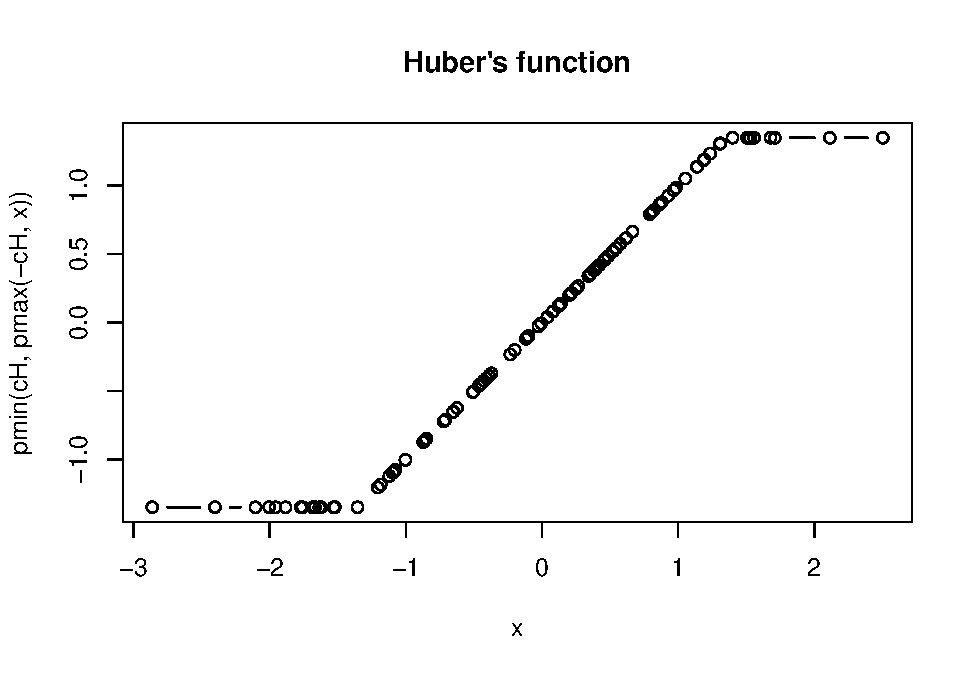
\includegraphics{TudodoR_files/figure-latex/unnamed-chunk-14-1.pdf}

\begin{verbatim}
## 
## min> cut01 <- function(x) pmax(pmin(x, 1), 0)
## 
## min> curve(      x^2 - 1/4, -1.4, 1.5, col = 2)
\end{verbatim}

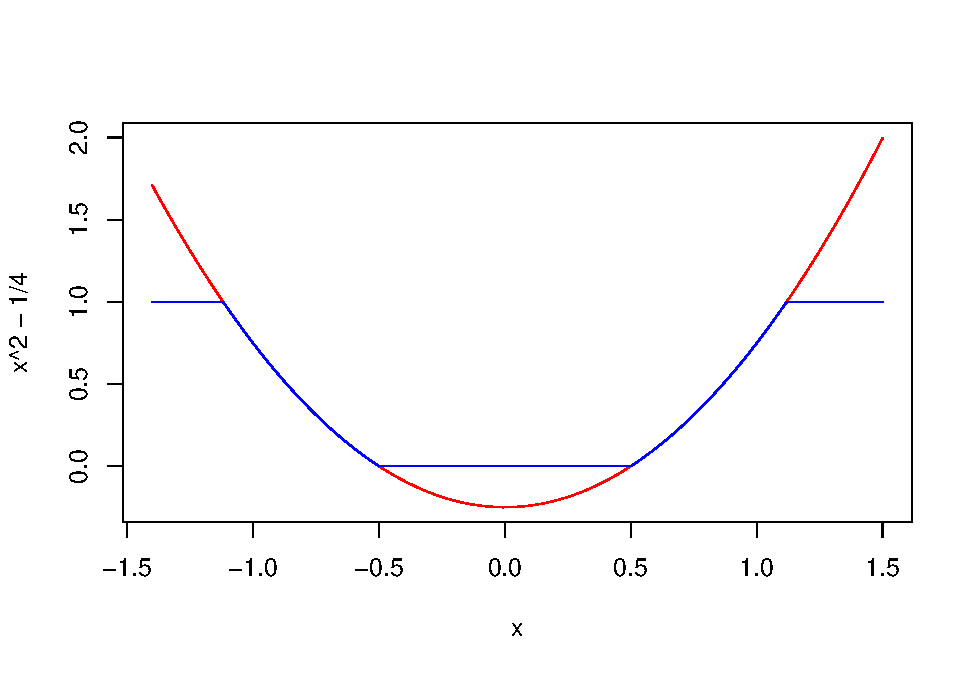
\includegraphics{TudodoR_files/figure-latex/unnamed-chunk-14-2.pdf}

\begin{verbatim}
## 
## min> curve(cut01(x^2 - 1/4), col = "blue", add = TRUE, n = 500)
## 
## min> ## pmax(), pmin() preserve attributes of *first* argument
## min> D <- diag(x = (3:1)/4) ; n0 <- numeric()
## 
## min> stopifnot(identical(D,  cut01(D) ),
## min+           identical(n0, cut01(n0)),
## min+           identical(n0, cut01(NULL)),
## min+           identical(n0, pmax(3:1, n0, 2)),
## min+           identical(n0, pmax(n0, 4)))
\end{verbatim}

\hypertarget{referencia}{%
\section{Referência}\label{referencia}}

MELO, M. P.; PETERNELI, L. A. \textbf{Conhecendo o R: Um visão mais que estatística}. Viçosa, MG: UFV, 2013. 222p.

\textbf{Prof.~Paulo Justiniando Ribeiro} \textgreater{}\url{http://www.leg.ufpr.br/~paulojus/}\textless{}

\textbf{Prof.~Adriano Azevedo Filho} \textgreater{}\url{http://rpubs.com/adriano/esalq2012inicial}\textless{}

\textbf{Prof.~Fernando de Pol Mayer} \textgreater{}\url{https://fernandomayer.github.io/ce083-2016-2/}\textless{}

\textbf{Site Interativo Datacamp} \textgreater{}\url{https://www.datacamp.com/}\textless{}

\hypertarget{estruturas-de-dados}{%
\chapter{Estruturas de Dados}\label{estruturas-de-dados}}

Este segundo Capitulo foi baseado no curso on-line \emph{Code School Try R} e no livro \href{https://www.editoraufv.com.br/produto/conhecendo-o-r-uma-visao-mais-que-estatistica/1109294}{\textbf{Conhecendo o R: Um visão mais que estatística}}, modificações foram realizadas utilizando outros materiais que se encontram referenciado no final do Capitulo.

\hypertarget{vetor}{%
\section{Vetor}\label{vetor}}

Um vetor é simplesmente uma lista de valores.
A maneira mais simples de usar um vetor é usando o comando \texttt{c()}, que concatena elementos num mesmo objeto.
Exemplo

\begin{Shaded}
\begin{Highlighting}[]
\NormalTok{x<-}\StringTok{ }\KeywordTok{c}\NormalTok{(}\DecValTok{2}\NormalTok{,}\DecValTok{3}\NormalTok{,}\DecValTok{5}\NormalTok{,}\DecValTok{7}\NormalTok{,}\DecValTok{11}\NormalTok{) }
\NormalTok{x}
\end{Highlighting}
\end{Shaded}

\begin{verbatim}
## [1]  2  3  5  7 11
\end{verbatim}

Os argumentos de \texttt{c()} podem ser tanto elementos únicos quanto outros objetos. Adicione três números no \textbf{vetor x}

\begin{Shaded}
\begin{Highlighting}[]
\NormalTok{y<-}\StringTok{ }\KeywordTok{c}\NormalTok{(x,}\DecValTok{13}\NormalTok{,}\DecValTok{17}\NormalTok{,}\DecValTok{19}\NormalTok{)}
\NormalTok{y}
\end{Highlighting}
\end{Shaded}

\begin{verbatim}
## [1]  2  3  5  7 11 13 17 19
\end{verbatim}

\hypertarget{vetores-de-sequencia}{%
\subsection{Vetores de Sequência}\label{vetores-de-sequencia}}

Se você precisa de um vetor com uma sequência de números, você pode cria-lo com a notação \emph{start:end}. Vamos fazer um vetor com valores de 1 a 7:

\begin{Shaded}
\begin{Highlighting}[]
\DecValTok{1}\OperatorTok{:}\DecValTok{7}
\end{Highlighting}
\end{Shaded}

\begin{verbatim}
## [1] 1 2 3 4 5 6 7
\end{verbatim}

Uma maneira mais versátil de fazer sequências é chamar a função \texttt{seq}. Vamos fazer o mesmo com \texttt{seq\ ()} :

\begin{Shaded}
\begin{Highlighting}[]
\KeywordTok{seq}\NormalTok{(}\DecValTok{1}\OperatorTok{:}\DecValTok{7}\NormalTok{)}
\end{Highlighting}
\end{Shaded}

\begin{verbatim}
## [1] 1 2 3 4 5 6 7
\end{verbatim}

A função \texttt{seq} também permite que você use incrementos diferentes de 1. Experimente com etapas de 0.5.

\begin{Shaded}
\begin{Highlighting}[]
\KeywordTok{seq}\NormalTok{(}\DecValTok{1}\NormalTok{,}\DecValTok{7}\NormalTok{,}\FloatTok{0.5}\NormalTok{)}
\end{Highlighting}
\end{Shaded}

\begin{verbatim}
##  [1] 1.0 1.5 2.0 2.5 3.0 3.5 4.0 4.5 5.0 5.5 6.0 6.5 7.0
\end{verbatim}

\begin{Shaded}
\begin{Highlighting}[]
\KeywordTok{seq}\NormalTok{(}\DecValTok{7}\NormalTok{,}\DecValTok{1}\NormalTok{,}\OperatorTok{-}\FloatTok{0.5}\NormalTok{) }
\end{Highlighting}
\end{Shaded}

\begin{verbatim}
##  [1] 7.0 6.5 6.0 5.5 5.0 4.5 4.0 3.5 3.0 2.5 2.0 1.5 1.0
\end{verbatim}

Todo objeto possui atributos intrínsecos: tipo e tamanho. Com relação ao tipo ele pode ser: \textbf{numérico}, \textbf{caractere}, \textbf{complexo} e \textbf{lógico}. Existem outros tipos, como por exemplo, funções ou expressões, porém esses não representam dados.
As funções \texttt{mode()} e \texttt{length()} mostram o tipo e tamanho de um objeto, respectivamente.

\begin{Shaded}
\begin{Highlighting}[]
\NormalTok{z<-}\KeywordTok{c}\NormalTok{(}\DecValTok{1}\NormalTok{,}\DecValTok{3}\NormalTok{,}\DecValTok{5}\NormalTok{,}\DecValTok{7}\NormalTok{,}\DecValTok{11}\NormalTok{) }
\KeywordTok{mode}\NormalTok{ (z)}
\end{Highlighting}
\end{Shaded}

\begin{verbatim}
## [1] "numeric"
\end{verbatim}

\begin{Shaded}
\begin{Highlighting}[]
\KeywordTok{length}\NormalTok{(z)}
\end{Highlighting}
\end{Shaded}

\begin{verbatim}
## [1] 5
\end{verbatim}

\begin{Shaded}
\begin{Highlighting}[]
\NormalTok{a <-}\StringTok{ "Angela"}
\NormalTok{b<-}\OtherTok{TRUE}\NormalTok{; }
\NormalTok{c<-8i }\CommentTok{#objetos com tipos diferentes}
\KeywordTok{mode}\NormalTok{(a); }
\end{Highlighting}
\end{Shaded}

\begin{verbatim}
## [1] "character"
\end{verbatim}

\begin{Shaded}
\begin{Highlighting}[]
\KeywordTok{mode}\NormalTok{(b); }
\end{Highlighting}
\end{Shaded}

\begin{verbatim}
## [1] "logical"
\end{verbatim}

\begin{Shaded}
\begin{Highlighting}[]
\KeywordTok{mode}\NormalTok{(c) }\CommentTok{#exibe os atributos "tipo" dos objetos }
\end{Highlighting}
\end{Shaded}

\begin{verbatim}
## [1] "complex"
\end{verbatim}

Se o vetor é muito longo e não ``cabe'' em uma linha o R vai usar as linhas seguintes para continuar imprimindo o vetor.

\begin{Shaded}
\begin{Highlighting}[]
\NormalTok{longo<-}\DecValTok{100}\OperatorTok{:}\DecValTok{50} \CommentTok{#sequência decrescente de 100 a 50}
\NormalTok{longo }\CommentTok{#exibe o conteúdo do objeto }
\end{Highlighting}
\end{Shaded}

\begin{verbatim}
##  [1] 100  99  98  97  96  95  94  93  92  91  90  89  88  87  86  85  84
## [18]  83  82  81  80  79  78  77  76  75  74  73  72  71  70  69  68  67
## [35]  66  65  64  63  62  61  60  59  58  57  56  55  54  53  52  51  50
\end{verbatim}

Os números entre colchetes não fazem parte do objeto e indica a posição do vetor naquele ponto. Pode-se ver que {[}1{]} indica que o primeiro elemento do vetor estão naquela linha, {[}17{]} indica que a linha seguinte começa pelo décimo setimo elemento do vetor e
assim por diante.

Você pode recuperar um valor individual dentro de um vetor fornecendo seu índice numérico entre colchetes. Tente obter o valor 18:

\begin{Shaded}
\begin{Highlighting}[]
\NormalTok{longo[}\DecValTok{18}\NormalTok{]}
\end{Highlighting}
\end{Shaded}

\begin{verbatim}
## [1] 83
\end{verbatim}

Muitas línguagem de programação iniciam índices de matriz em 0, mas os índices vetoriais de R começam em 1. Obtenha o primeiro valor digitando:

\begin{Shaded}
\begin{Highlighting}[]
\NormalTok{longo[}\DecValTok{1}\NormalTok{]}
\end{Highlighting}
\end{Shaded}

\begin{verbatim}
## [1] 100
\end{verbatim}

Você pode atribuir novos valores dentro de um vetor existente. Tente mudar o terceiro valor \textbf{28}:

\begin{Shaded}
\begin{Highlighting}[]
\NormalTok{longo [}\DecValTok{3}\NormalTok{] <-}\StringTok{ }\DecValTok{28}
\end{Highlighting}
\end{Shaded}

Se você adicionar novos valores ao final, o vetor aumentará para acomodá-los. Vamos adicionar um valor no final

\begin{Shaded}
\begin{Highlighting}[]
\NormalTok{longo[}\DecValTok{101}\NormalTok{] <-}\StringTok{ }\DecValTok{83}
\end{Highlighting}
\end{Shaded}

Você pode usar um vetor entre os colchetes para acessar vários valores. Tente obter a primeira e a terceira palavras

\begin{Shaded}
\begin{Highlighting}[]
\NormalTok{longo[}\KeywordTok{c}\NormalTok{(}\DecValTok{1}\NormalTok{,}\DecValTok{3}\NormalTok{)]}
\end{Highlighting}
\end{Shaded}

\begin{verbatim}
## [1] 100  28
\end{verbatim}

Isso significa que você pode recuperar intervalos de valores. Obter a segunda a quarta palavras:

\begin{Shaded}
\begin{Highlighting}[]
\NormalTok{longo[}\DecValTok{2}\OperatorTok{:}\DecValTok{4}\NormalTok{]}
\end{Highlighting}
\end{Shaded}

\begin{verbatim}
## [1] 99 28 97
\end{verbatim}

Você também pode definir intervalos de valores; apenas forneça os valores em um vetor. Adicione valores 5 a 7:

\begin{Shaded}
\begin{Highlighting}[]
\NormalTok{longo[}\DecValTok{5}\OperatorTok{:}\DecValTok{7}\NormalTok{] <-}\StringTok{ }\KeywordTok{c}\NormalTok{(}\DecValTok{42}\NormalTok{,}\DecValTok{52}\NormalTok{,}\DecValTok{75}\NormalTok{)}
\end{Highlighting}
\end{Shaded}

Agora tente acessar o oitavo valor do vetor:

\begin{Shaded}
\begin{Highlighting}[]
\NormalTok{longo[}\DecValTok{8}\NormalTok{]}
\end{Highlighting}
\end{Shaded}

\begin{verbatim}
## [1] 93
\end{verbatim}

\hypertarget{nomes-de-vetores}{%
\subsection{Nomes de vetores}\label{nomes-de-vetores}}

Para esse desafio, criaremos um vetor de 3 itens e armazená-lo na variável solo.
Você pode atribuir nomes aos elementos de um vetor passando um segundo vetor preenchido com os nomes com a função \texttt{names\ ()}, assim:

\begin{Shaded}
\begin{Highlighting}[]
\NormalTok{solo <-}\StringTok{ }\DecValTok{1}\OperatorTok{:}\DecValTok{3}
\KeywordTok{names}\NormalTok{(solo) <-}\StringTok{ }\KeywordTok{c}\NormalTok{(}\StringTok{"Argila"}\NormalTok{, }\StringTok{"Areia"}\NormalTok{,}\StringTok{"Silte"}\NormalTok{ )}
\NormalTok{solo}
\end{Highlighting}
\end{Shaded}

\begin{verbatim}
## Argila  Areia  Silte 
##      1      2      3
\end{verbatim}

Agora, defina o valor atual para o \emph{silte} para um valor diferente usando o nome em vez da posição.

\begin{Shaded}
\begin{Highlighting}[]
\NormalTok{solo[}\StringTok{"Silte"}\NormalTok{]<-}\DecValTok{20}
\end{Highlighting}
\end{Shaded}

\hypertarget{plotando-um-vetor}{%
\subsection{Plotando um vetor}\label{plotando-um-vetor}}

A função \texttt{barplot\ ()} desenha um gráfico de barras com os valores de um vetor. Vamos criar um novo vetor para você e armazená-lo na variável chuva.

Agora, tente passar o vetor para a função \texttt{barplot}:

\begin{Shaded}
\begin{Highlighting}[]
\NormalTok{chuva <-}\StringTok{ }\KeywordTok{c}\NormalTok{(}\DecValTok{20}\NormalTok{,}\DecValTok{50}\NormalTok{,}\DecValTok{85}\NormalTok{)}
\KeywordTok{barplot}\NormalTok{(chuva)}
\end{Highlighting}
\end{Shaded}

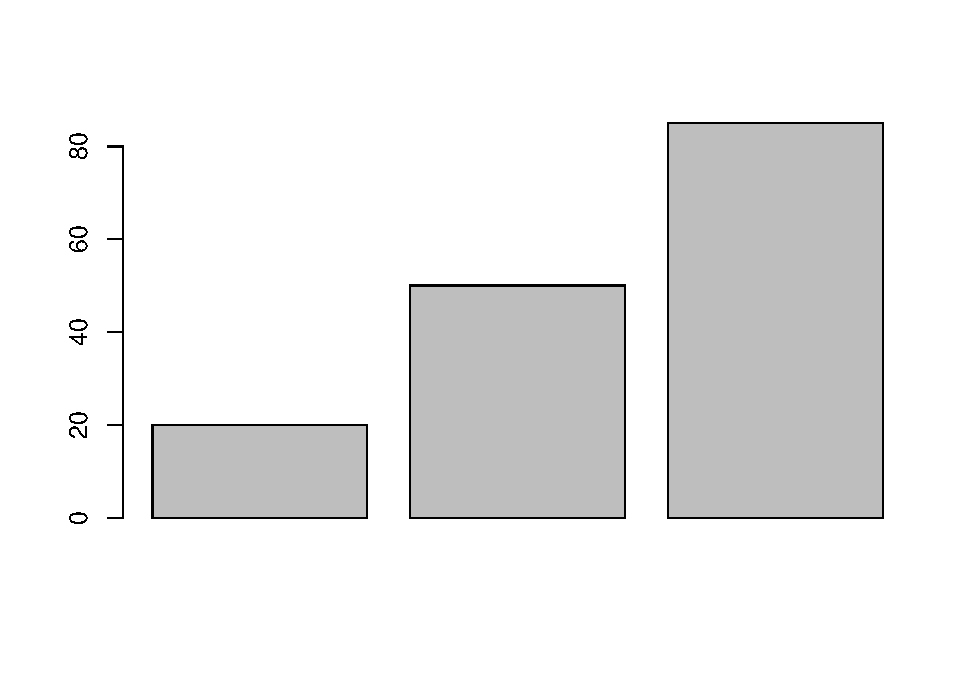
\includegraphics{TudodoR_files/figure-latex/unnamed-chunk-32-1.pdf}

Se você atribuir nomes aos valores do vetor, o R usará esses nomes como rótulos no gráfico da barra. Vamos usar a função \texttt{names\ ()} novamente:

\begin{Shaded}
\begin{Highlighting}[]
\KeywordTok{names}\NormalTok{(chuva)<-}\StringTok{ }\KeywordTok{c}\NormalTok{(}\StringTok{"Rondonópolis", "}\NormalTok{Maringá}\StringTok{", "}\NormalTok{Cruzeiro do Sul}\StringTok{")}
\end{Highlighting}
\end{Shaded}

Agora, se você digitar \texttt{barplot\ (chuva)} com o vetor novamente, você verá os rótulos:

\begin{Shaded}
\begin{Highlighting}[]
\KeywordTok{barplot}\NormalTok{(chuva)}
\end{Highlighting}
\end{Shaded}

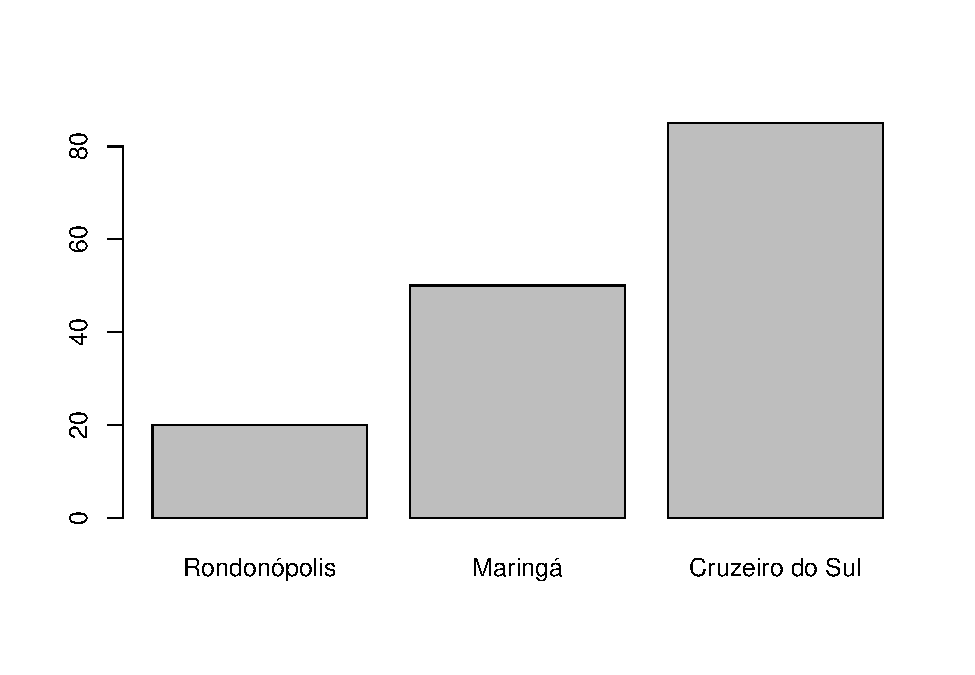
\includegraphics{TudodoR_files/figure-latex/unnamed-chunk-34-1.pdf}

Agora, tente chamar \texttt{barplot} em um vetor de números inteiros que variam de 1 a 100:

\begin{Shaded}
\begin{Highlighting}[]
\KeywordTok{barplot}\NormalTok{(}\DecValTok{1}\OperatorTok{:}\DecValTok{100}\NormalTok{)}
\end{Highlighting}
\end{Shaded}

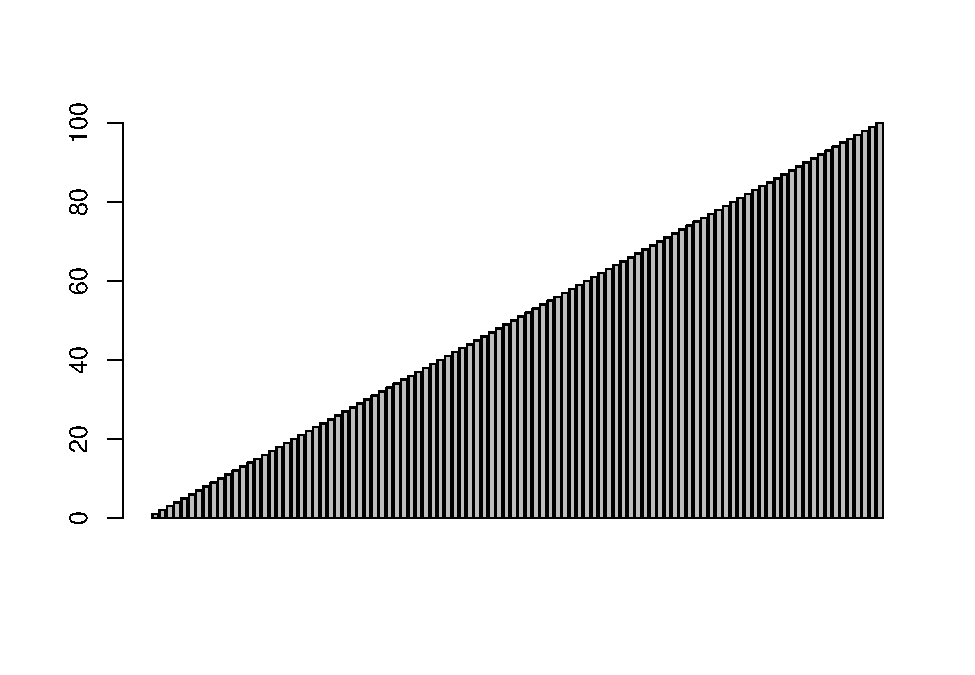
\includegraphics{TudodoR_files/figure-latex/unnamed-chunk-35-1.pdf}

\hypertarget{operacoes-matematicas}{%
\subsection{Operações matemáticas}\label{operacoes-matematicas}}

A maioria das operações aritméticas funcionam tão bem em vetores quanto em valores únicos. Vamos fazer outro vetor de exemplo para você trabalhar e armazená-lo a variável \textbf{a}

Se você adicionar um escalar (um único valor) a um vetor, o escalar será adicionado a cada valor no vetor, retornando um novo vetor com os resultados. Tente adicionar 1 a cada elemento em nosso vetor:

\begin{Shaded}
\begin{Highlighting}[]
\NormalTok{a <-}\StringTok{ }\KeywordTok{c}\NormalTok{(}\DecValTok{1}\NormalTok{, }\DecValTok{2}\NormalTok{, }\DecValTok{3}\NormalTok{)}
\NormalTok{a }\OperatorTok{+}\StringTok{ }\DecValTok{1}
\end{Highlighting}
\end{Shaded}

\begin{verbatim}
## [1] 2 3 4
\end{verbatim}

O mesmo se aplica na divisão, multiplicação ou qualquer outra aritmética básica. Tente dividir nosso vetor por 2:

\begin{Shaded}
\begin{Highlighting}[]
\NormalTok{a }\OperatorTok{/}\StringTok{ }\DecValTok{2}
\end{Highlighting}
\end{Shaded}

\begin{verbatim}
## [1] 0.5 1.0 1.5
\end{verbatim}

Agora, tente multiplicar nosso vetor por 2:

\begin{Shaded}
\begin{Highlighting}[]
\NormalTok{a}\OperatorTok{*}\DecValTok{2}
\end{Highlighting}
\end{Shaded}

\begin{verbatim}
## [1] 2 4 6
\end{verbatim}

Se você adicionar dois vetores, R irá tirar cada valor de cada vetor e adicioná-los. Vamos fazer um segundo vetor para você experimentar e armazená-lo na variável \textbf{b}

Tente adicioná-lo ao vetor \textbf{a}:

\begin{Shaded}
\begin{Highlighting}[]
\NormalTok{b <-}\StringTok{ }\KeywordTok{c}\NormalTok{(}\DecValTok{4}\NormalTok{,}\DecValTok{5}\NormalTok{,}\DecValTok{6}\NormalTok{)}
\NormalTok{a}\OperatorTok{+}\NormalTok{b}
\end{Highlighting}
\end{Shaded}

\begin{verbatim}
## [1] 5 7 9
\end{verbatim}

Agora tente subtrair b de a:

\begin{Shaded}
\begin{Highlighting}[]
\NormalTok{a}\OperatorTok{-}\NormalTok{b}
\end{Highlighting}
\end{Shaded}

\begin{verbatim}
## [1] -3 -3 -3
\end{verbatim}

Você também pode tirar dois vetores e comparar cada item. Veja quais valores nos vetores são iguais aos de um segundo vetor

\begin{Shaded}
\begin{Highlighting}[]
\NormalTok{a }\OperatorTok{==}\StringTok{ }\KeywordTok{c}\NormalTok{(}\DecValTok{1}\NormalTok{, }\DecValTok{99}\NormalTok{, }\DecValTok{3}\NormalTok{)}
\end{Highlighting}
\end{Shaded}

\begin{verbatim}
## [1]  TRUE FALSE  TRUE
\end{verbatim}

Observe que R não testou se os vetores inteiros eram iguais; verificou cada valor no vetor a contra o valor no mesmo índice no nosso novo vetor.

Verifique se cada valor nos vetores são menores que o valor correspondente em outro vetor:

\begin{Shaded}
\begin{Highlighting}[]
\NormalTok{a }\OperatorTok{<}\StringTok{ }\KeywordTok{c}\NormalTok{(}\DecValTok{1}\NormalTok{, }\DecValTok{99}\NormalTok{, }\DecValTok{3}\NormalTok{)}
\end{Highlighting}
\end{Shaded}

\begin{verbatim}
## [1] FALSE  TRUE FALSE
\end{verbatim}

Funções que normalmente funcionam com escalares também podem operar em cada elemento de um vetor. Tente obter o seno de cada valor em nosso vetor:

\begin{Shaded}
\begin{Highlighting}[]
\KeywordTok{sin}\NormalTok{(a)}
\end{Highlighting}
\end{Shaded}

\begin{verbatim}
## [1] 0.8414710 0.9092974 0.1411200
\end{verbatim}

Agora tente obter as raízes quadradas com a função \texttt{sqrt}:

\begin{Shaded}
\begin{Highlighting}[]
\KeywordTok{sqrt}\NormalTok{(a)}
\end{Highlighting}
\end{Shaded}

\begin{verbatim}
## [1] 1.000000 1.414214 1.732051
\end{verbatim}

\hypertarget{parcelas-de-dispersao}{%
\subsection{Parcelas de dispersão}\label{parcelas-de-dispersao}}

A função \texttt{plot} leva dois vetores, um para valores X e um para valores Y, e desenha um gráfico deles.

Vamos desenhar um gráfico que mostra a relação de números e seus senos.

Primeiro, precisaremos de alguns dados de amostra. Criaremos um vetor com alguns valores fracionários entre 0 e 20, e armazenó-lo na variável x. E na variável y um segundo vetor com os senos de x:

\begin{Shaded}
\begin{Highlighting}[]
\NormalTok{x <-}\StringTok{ }\KeywordTok{seq}\NormalTok{(}\DecValTok{1}\NormalTok{, }\DecValTok{20}\NormalTok{, }\FloatTok{0.1}\NormalTok{)}
\NormalTok{y<-}\KeywordTok{sin}\NormalTok{(x)}
\end{Highlighting}
\end{Shaded}

Em seguida, basta chamar a função \texttt{plot} com seus dois vetores:

\begin{Shaded}
\begin{Highlighting}[]
\KeywordTok{plot}\NormalTok{(x, y)}
\end{Highlighting}
\end{Shaded}

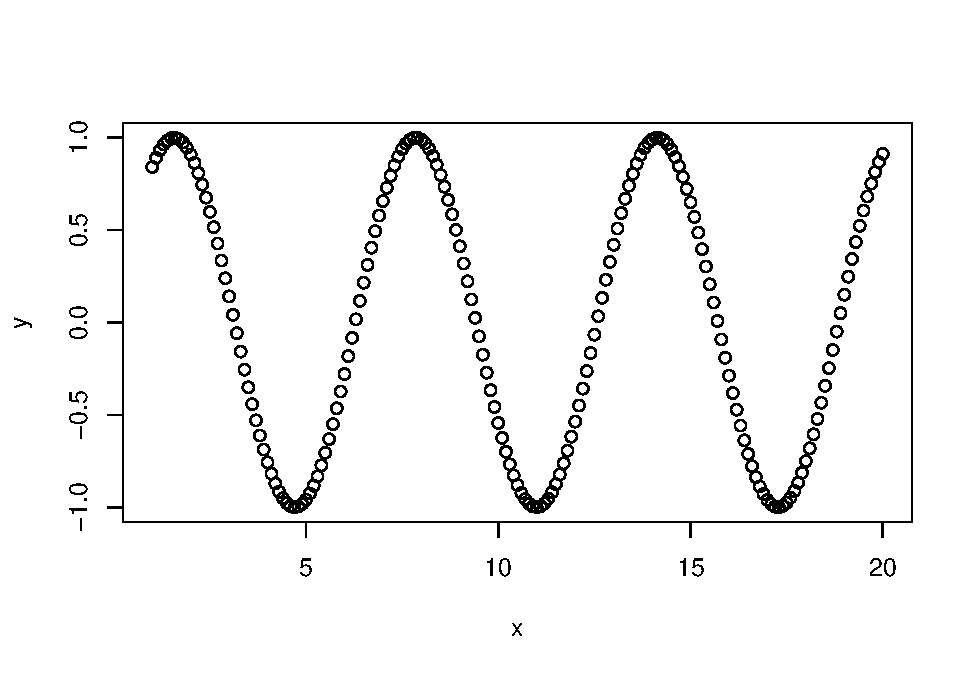
\includegraphics{TudodoR_files/figure-latex/unnamed-chunk-46-1.pdf}

Observa=se sobre o gráfico que os valores do primeiro argumento \textbf{(x)} são usados para o eixo horizontal, e os valores do segundo \textbf{(y)} para o vertical.

Vamos criar um vetor com alguns valores negativos e positivos para você e armazenó-lo na variável \textbf{valores}.

Também criaremos um segundo vetor com os valores absolutos do primeiro e armazenó-lo na variável \textbf{absoluto}.

Tente traçar os vetores, com os \textbf{valores} no eixo horizontal e no eixo vertical os absoluto.

\begin{Shaded}
\begin{Highlighting}[]
\NormalTok{valores <-}\StringTok{ }\DecValTok{-10}\OperatorTok{:}\DecValTok{10}
\NormalTok{absoluto<-}\StringTok{ }\KeywordTok{abs}\NormalTok{(valores)}
\KeywordTok{plot}\NormalTok{(valores, absoluto)}
\end{Highlighting}
\end{Shaded}

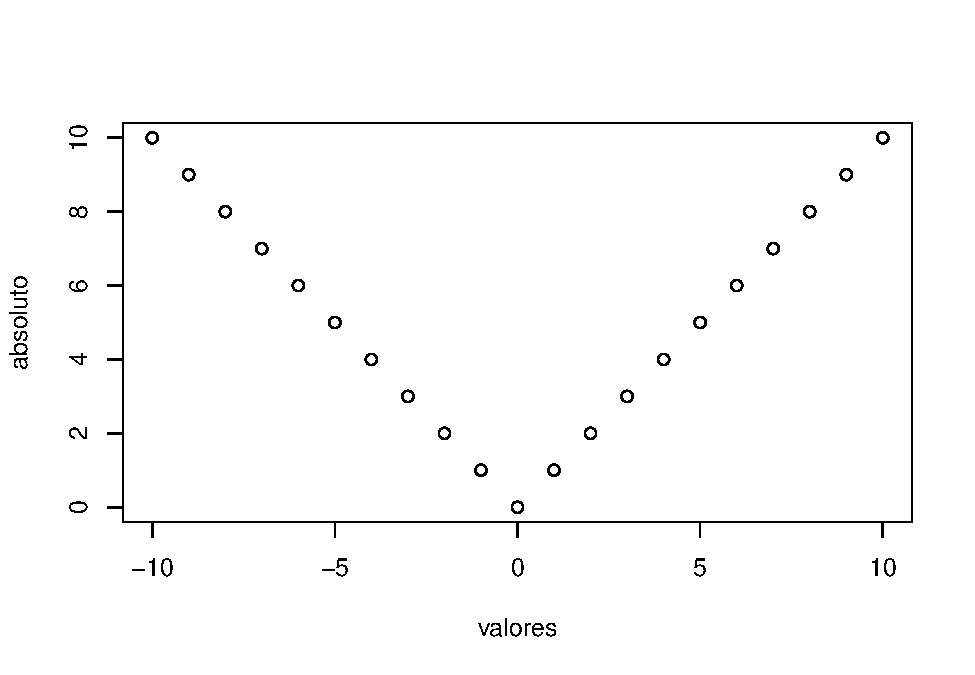
\includegraphics{TudodoR_files/figure-latex/unnamed-chunk-47-1.pdf}

\hypertarget{valores-faltantes}{%
\subsection{Valores Faltantes}\label{valores-faltantes}}

As vezes, ao trabalhar com dados de amostra, um determinado valor não está disponível. Mas não é uma boa idéia apenas tirar esses valores. R tem um valor que indica explicitamente uma amostra não estava disponível: \textbf{NA}. Muitas funções que funcionam com vetores tratam esse valor especialmente.

Vamos criar um vetor para você com uma amostra ausente e armazenó-lo na variével \textbf{a}.

Tente obter a soma de seus valores e veja qual é o resultado:

\begin{Shaded}
\begin{Highlighting}[]
\NormalTok{a <-}\StringTok{ }\KeywordTok{c}\NormalTok{(}\DecValTok{1}\NormalTok{, }\DecValTok{3}\NormalTok{, }\OtherTok{NA}\NormalTok{, }\DecValTok{7}\NormalTok{, }\DecValTok{9}\NormalTok{)}
\KeywordTok{sum}\NormalTok{(a)}
\end{Highlighting}
\end{Shaded}

\begin{verbatim}
## [1] NA
\end{verbatim}

A soma é considerada \emph{``não disponível''} por padrão porque um dos valores do vetor foi \textbf{NA}.

Lembre-se desse comando para mostrar ajuda para uma função. Apresente a ajuda para a função \texttt{sum}:

\begin{Shaded}
\begin{Highlighting}[]
\KeywordTok{help}\NormalTok{(sum)}
\end{Highlighting}
\end{Shaded}

Como você vê na documentação, \texttt{sum} pode tomar um argumento opcional \textbf{na.rm},. ? configurado \textbf{FALSE} por padrão, mas se você configurá-lo com \textbf{TRUE}, todos os argumentos \textbf{NA} serão removidos do vetor antes do cálculo ser executado.

Tente rondar \texttt{sum} novamente, com o \textbf{na.rm} conjunto para \textbf{TRUE}:

\begin{Shaded}
\begin{Highlighting}[]
\KeywordTok{sum}\NormalTok{(a, }\DataTypeTok{na.rm =}\NormalTok{ T)}
\end{Highlighting}
\end{Shaded}

\begin{verbatim}
## [1] 20
\end{verbatim}

\hypertarget{matrizes}{%
\section{Matrizes}\label{matrizes}}

Há varias formas de criar uma matriz. O comando \texttt{matriz()} recebe um vetor como argumento e o transfoma em uma matrix de acordo com as dimensões.
Vamos fazer uma matriz de 3 linhas de altura por 4 colunas de largura, com todos os seus campos definidos 0.

\begin{Shaded}
\begin{Highlighting}[]
\KeywordTok{matrix}\NormalTok{(}\DecValTok{0}\NormalTok{,}\DecValTok{3}\NormalTok{,}\DecValTok{4}\NormalTok{)}
\end{Highlighting}
\end{Shaded}

\begin{verbatim}
##      [,1] [,2] [,3] [,4]
## [1,]    0    0    0    0
## [2,]    0    0    0    0
## [3,]    0    0    0    0
\end{verbatim}

Você também pode usar um vetor para inicializar o valor de uma matriz. Para preencher uma matriz de 3x4, você precisará de um vetor de 12 itens.

\begin{Shaded}
\begin{Highlighting}[]
\NormalTok{a <-}\StringTok{ }\NormalTok{(}\DecValTok{1}\OperatorTok{:}\DecValTok{12}\NormalTok{)}

\KeywordTok{print}\NormalTok{ (a)}
\end{Highlighting}
\end{Shaded}

\begin{verbatim}
##  [1]  1  2  3  4  5  6  7  8  9 10 11 12
\end{verbatim}

Agora chame matrix com o vetor, o número de linhas e o número de colunas:

\begin{Shaded}
\begin{Highlighting}[]
\KeywordTok{matrix}\NormalTok{ (a,}\CommentTok{# chama o vetor}
        \DecValTok{3}\NormalTok{,}\CommentTok{# linha}
        \DecValTok{4}\NormalTok{) }\CommentTok{#coluna}
\end{Highlighting}
\end{Shaded}

\begin{verbatim}
##      [,1] [,2] [,3] [,4]
## [1,]    1    4    7   10
## [2,]    2    5    8   11
## [3,]    3    6    9   12
\end{verbatim}

Você também pode usar um vetor para inicializar o valor de uma matriz. Para preencher uma matriz 3x4, você precisará de um vetor de 12 itens. Nós vamos fazer isso para você agora:

\begin{Shaded}
\begin{Highlighting}[]
\NormalTok{a <-}\DecValTok{1}\OperatorTok{:}\DecValTok{12}
\NormalTok{a}
\end{Highlighting}
\end{Shaded}

\begin{verbatim}
##  [1]  1  2  3  4  5  6  7  8  9 10 11 12
\end{verbatim}

Agora chame \textbf{matrix} com o vetor, o número de linhas e o número de colunas:

\begin{Shaded}
\begin{Highlighting}[]
\KeywordTok{matrix}\NormalTok{ (a,}\DecValTok{3}\NormalTok{,}\DecValTok{4}\NormalTok{)}
\end{Highlighting}
\end{Shaded}

\begin{verbatim}
##      [,1] [,2] [,3] [,4]
## [1,]    1    4    7   10
## [2,]    2    5    8   11
## [3,]    3    6    9   12
\end{verbatim}

\hypertarget{outras-formas}{%
\subsection{Outras formas}\label{outras-formas}}

\begin{Shaded}
\begin{Highlighting}[]
\KeywordTok{matrix}\NormalTok{ (a, }\DecValTok{3}\NormalTok{)}
\end{Highlighting}
\end{Shaded}

\begin{verbatim}
##      [,1] [,2] [,3] [,4]
## [1,]    1    4    7   10
## [2,]    2    5    8   11
## [3,]    3    6    9   12
\end{verbatim}

Note que as matrizes são preenchidas ao longo das colunas. Para que a matriz seja preenchida por linhas deve-se alterar o argumento \textbf{byrow}, que, por padrão, está definido como \textbf{FALSE}, passe para \textbf{TRUE}

\begin{Shaded}
\begin{Highlighting}[]
\KeywordTok{matrix}\NormalTok{(a,}\DecValTok{3}\NormalTok{, }\DataTypeTok{byrow=}\NormalTok{T)}
\end{Highlighting}
\end{Shaded}

\begin{verbatim}
##      [,1] [,2] [,3] [,4]
## [1,]    1    2    3    4
## [2,]    5    6    7    8
## [3,]    9   10   11   12
\end{verbatim}

Os valores do vetor são copiados para a nova matriz, um por um. Você também pode reformular o próprio \textbf{vetor} em uma \textbf{matriz}. Crie um vetor de 8 itens:

\begin{Shaded}
\begin{Highlighting}[]
\NormalTok{foliar <-}\StringTok{ }\DecValTok{1}\OperatorTok{:}\DecValTok{8}
\end{Highlighting}
\end{Shaded}

A função \texttt{dim} define as \textbf{dim}ensões para uma matriz. Ele aceita um vetor com o número de linhas e o n?mero de colunas a serem atribu?das.
Atribua novas dimens?es para \textbf{foliar} passando um vetor especificando 2 linhas e 4 colunas ( c(2, 4)):

\begin{Shaded}
\begin{Highlighting}[]
\KeywordTok{dim}\NormalTok{(foliar) <-}\StringTok{ }\KeywordTok{c}\NormalTok{(}\DecValTok{2}\NormalTok{,}\DecValTok{4}\NormalTok{)}
\end{Highlighting}
\end{Shaded}

O vetor não é mais unidimensional. Foi convertido, no local, para uma matriz.
Agora, use a função \textbf{matrix} para criar uma matriz \textbf{5x5}, com seus campos inicializados para qualquer valor que você desejar.

\begin{Shaded}
\begin{Highlighting}[]
\KeywordTok{matrix}\NormalTok{ (}\DecValTok{2}\NormalTok{,}\DecValTok{5}\NormalTok{,}\DecValTok{5}\NormalTok{)}
\end{Highlighting}
\end{Shaded}

\begin{verbatim}
##      [,1] [,2] [,3] [,4] [,5]
## [1,]    2    2    2    2    2
## [2,]    2    2    2    2    2
## [3,]    2    2    2    2    2
## [4,]    2    2    2    2    2
## [5,]    2    2    2    2    2
\end{verbatim}

\hypertarget{acesso-a-matriz}{%
\subsection{Acesso a Matriz}\label{acesso-a-matriz}}

Obter valores de matrizes não é diferente de vetores; você só precisa fornecer dois índices em vez de um. Abra a matriz foliar:

\begin{Shaded}
\begin{Highlighting}[]
\KeywordTok{print}\NormalTok{ (foliar)}
\end{Highlighting}
\end{Shaded}

\begin{verbatim}
##      [,1] [,2] [,3] [,4]
## [1,]    1    3    5    7
## [2,]    2    4    6    8
\end{verbatim}

Tente obter o valor da segunda linha na terceira coluna da matriz foliar;

\begin{Shaded}
\begin{Highlighting}[]
\NormalTok{foliar[}\DecValTok{2}\NormalTok{,}\DecValTok{3}\NormalTok{]}
\end{Highlighting}
\end{Shaded}

\begin{verbatim}
## [1] 6
\end{verbatim}

O valor da primeira linha da quarta coluna

\begin{Shaded}
\begin{Highlighting}[]
\NormalTok{foliar[}\DecValTok{1}\NormalTok{,}\DecValTok{4}\NormalTok{]}
\end{Highlighting}
\end{Shaded}

\begin{verbatim}
## [1] 7
\end{verbatim}

Você pode obter uma linha inteira da matriz omitindo o índice da coluna (mas mantenha a virgula). Tente recuperar a segunda linha:

\begin{Shaded}
\begin{Highlighting}[]
\NormalTok{foliar[}\DecValTok{2}\NormalTok{,]}
\end{Highlighting}
\end{Shaded}

\begin{verbatim}
## [1] 2 4 6 8
\end{verbatim}

Para obter uma coluna inteira, omita o índice da linha. Recupere a quarta coluna:

\begin{Shaded}
\begin{Highlighting}[]
\NormalTok{foliar[,}\DecValTok{4}\NormalTok{]}
\end{Highlighting}
\end{Shaded}

\begin{verbatim}
## [1] 7 8
\end{verbatim}

Você pode ler várias linhas ou colunas, fornecendo um vetor ou sequência com seus índices. Tente recuperar as colunas de 2 a 4:

\begin{Shaded}
\begin{Highlighting}[]
\NormalTok{foliar[,}\DecValTok{2}\OperatorTok{:}\DecValTok{4}\NormalTok{]}
\end{Highlighting}
\end{Shaded}

\begin{verbatim}
##      [,1] [,2] [,3]
## [1,]    3    5    7
## [2,]    4    6    8
\end{verbatim}

O comando \texttt{summary} pode ser usado para obter informações da matriz

\begin{Shaded}
\begin{Highlighting}[]
\KeywordTok{summary}\NormalTok{(foliar)}
\end{Highlighting}
\end{Shaded}

\begin{verbatim}
##        V1             V2             V3             V4      
##  Min.   :1.00   Min.   :3.00   Min.   :5.00   Min.   :7.00  
##  1st Qu.:1.25   1st Qu.:3.25   1st Qu.:5.25   1st Qu.:7.25  
##  Median :1.50   Median :3.50   Median :5.50   Median :7.50  
##  Mean   :1.50   Mean   :3.50   Mean   :5.50   Mean   :7.50  
##  3rd Qu.:1.75   3rd Qu.:3.75   3rd Qu.:5.75   3rd Qu.:7.75  
##  Max.   :2.00   Max.   :4.00   Max.   :6.00   Max.   :8.00
\end{verbatim}

Se desejar um resumo de todos os elementos da matriz, basta transformá-la em um vetor

\begin{Shaded}
\begin{Highlighting}[]
\KeywordTok{summary}\NormalTok{(}\KeywordTok{as.vector}\NormalTok{(foliar))}
\end{Highlighting}
\end{Shaded}

\begin{verbatim}
##    Min. 1st Qu.  Median    Mean 3rd Qu.    Max. 
##    1.00    2.75    4.50    4.50    6.25    8.00
\end{verbatim}

\hypertarget{visualizacoes-em-dados-matriciais}{%
\subsection{Visualizações em dados matriciais}\label{visualizacoes-em-dados-matriciais}}

Com um mapa de elevação. Tudo fica a 1 metro acima do nível do mar. Vamos criar uma matriz de 10 por 10 com todos os seus valores inicializados para 1 para você:

\begin{Shaded}
\begin{Highlighting}[]
\NormalTok{elevacao <-}\StringTok{ }\KeywordTok{matrix}\NormalTok{ (}\DecValTok{1}\NormalTok{,}\DecValTok{10}\NormalTok{,}\DecValTok{10}\NormalTok{)}
\end{Highlighting}
\end{Shaded}

Na quarta linha, sexta coluna, defina a elevação para 0:

\begin{Shaded}
\begin{Highlighting}[]
\NormalTok{elevacao [}\DecValTok{4}\NormalTok{, }\DecValTok{6}\NormalTok{] <-}\StringTok{ }\DecValTok{0}
\end{Highlighting}
\end{Shaded}

Mapa de contorno dos valores passando a matriz para a função \texttt{contour}

\begin{Shaded}
\begin{Highlighting}[]
\KeywordTok{contour}\NormalTok{(elevacao)}
\end{Highlighting}
\end{Shaded}

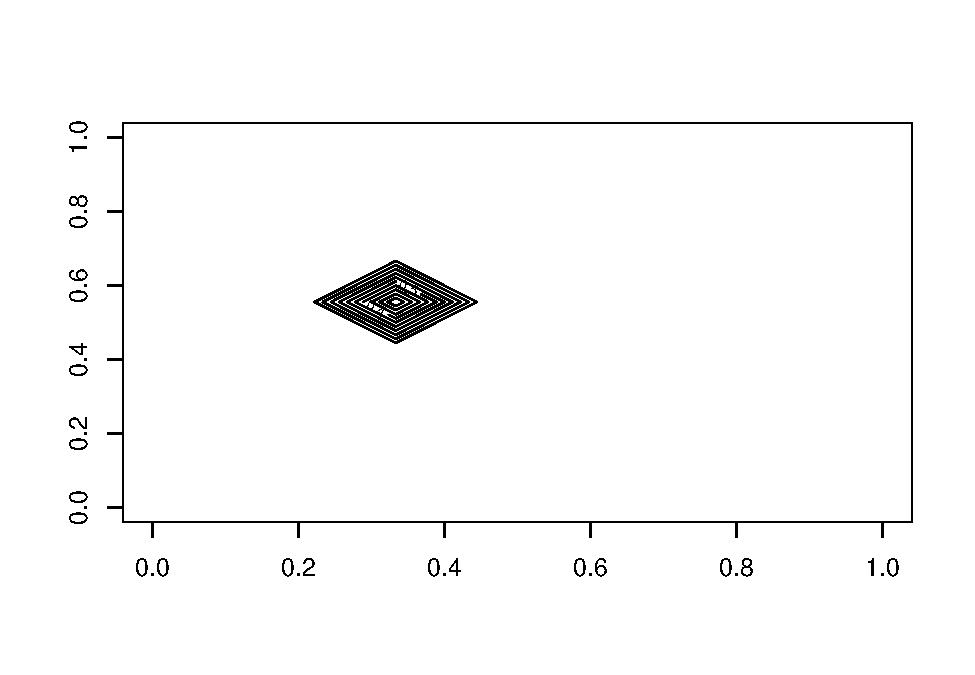
\includegraphics{TudodoR_files/figure-latex/unnamed-chunk-71-1.pdf}

Criar um gráfico em perspectiva 3D com a função \texttt{persp}:

\begin{Shaded}
\begin{Highlighting}[]
\KeywordTok{persp}\NormalTok{ (elevacao)}
\end{Highlighting}
\end{Shaded}

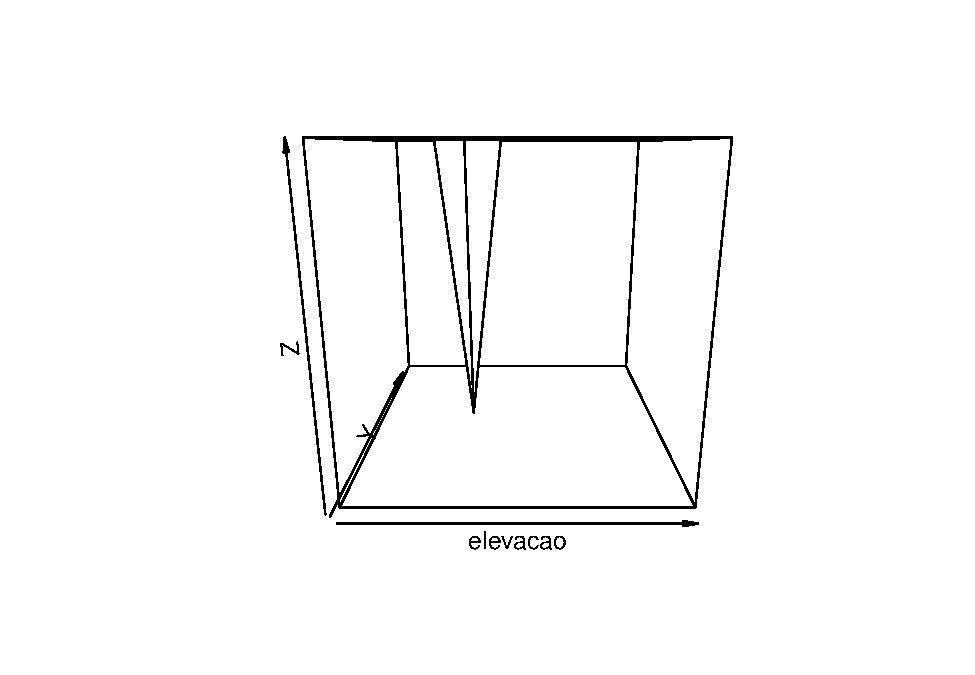
\includegraphics{TudodoR_files/figure-latex/unnamed-chunk-72-1.pdf}

Podemos consertar isso especificando nosso próprio valor para o parâmetro \textbf{expand}.

\begin{Shaded}
\begin{Highlighting}[]
\KeywordTok{persp}\NormalTok{ (elevacao, }\DataTypeTok{expand =}\FloatTok{0.2}\NormalTok{)}
\end{Highlighting}
\end{Shaded}

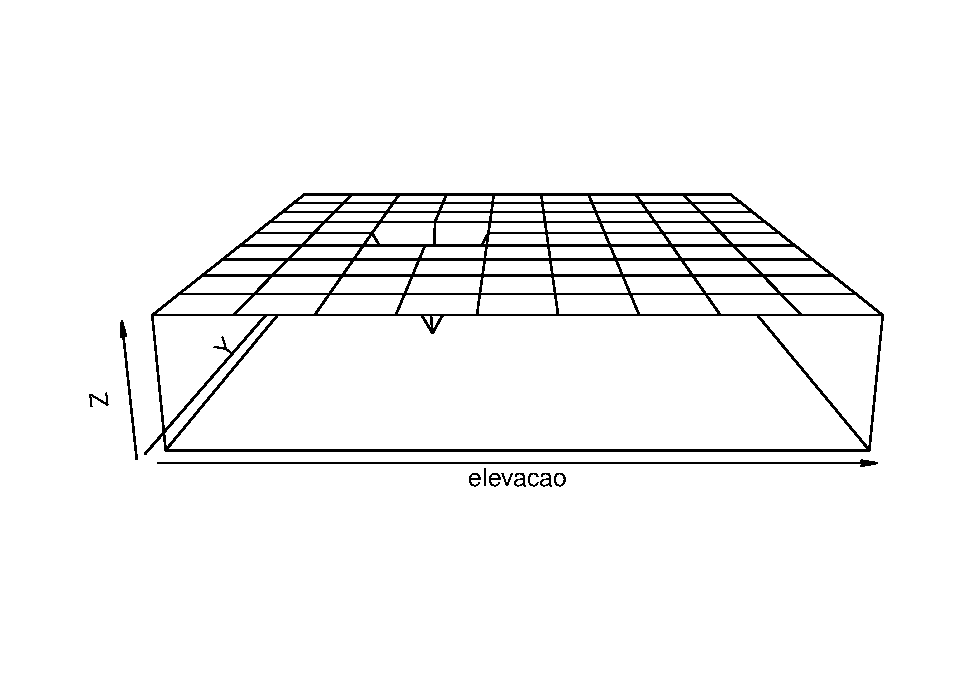
\includegraphics{TudodoR_files/figure-latex/unnamed-chunk-73-1.pdf}

R inclui alguns conjuntos de dados de amostra. Um deles é o \emph{volcanoum} mapa 3D de um vulcão adormecido da Nova Zelândia.

É simplesmente uma matriz de 87x61 com valores de elevão, mas mostra o poder das visualizações de matriz do R. Criar um mapa de calor:

\begin{Shaded}
\begin{Highlighting}[]
\KeywordTok{contour}\NormalTok{(volcano)}
\end{Highlighting}
\end{Shaded}

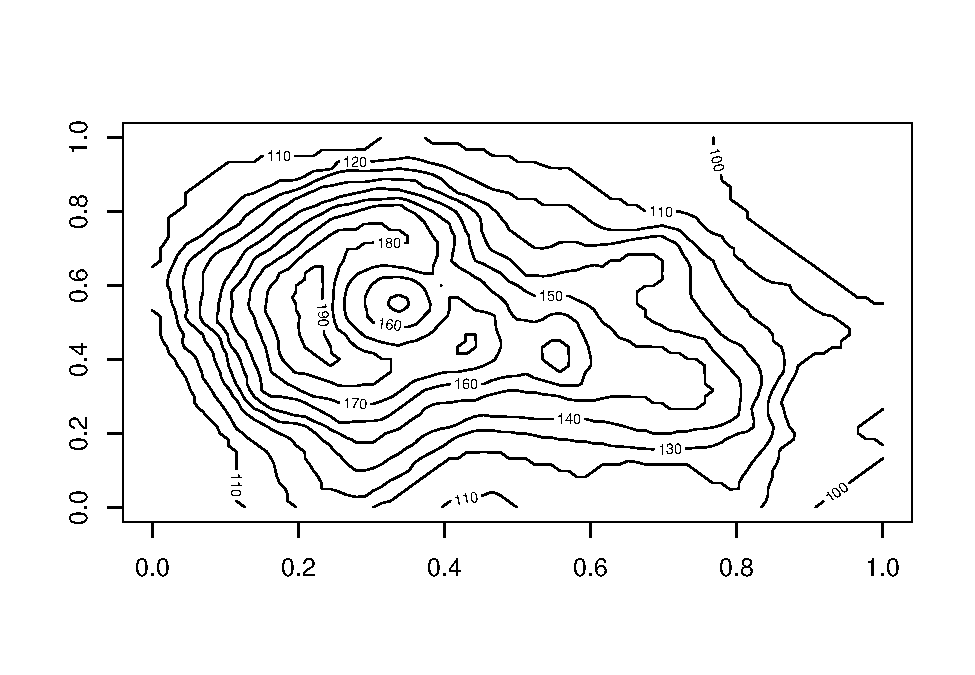
\includegraphics{TudodoR_files/figure-latex/unnamed-chunk-74-1.pdf}

Gráfico em perspectiva:

\begin{Shaded}
\begin{Highlighting}[]
\KeywordTok{persp}\NormalTok{(volcano, }\DataTypeTok{expand=}\FloatTok{0.2}\NormalTok{)}
\end{Highlighting}
\end{Shaded}

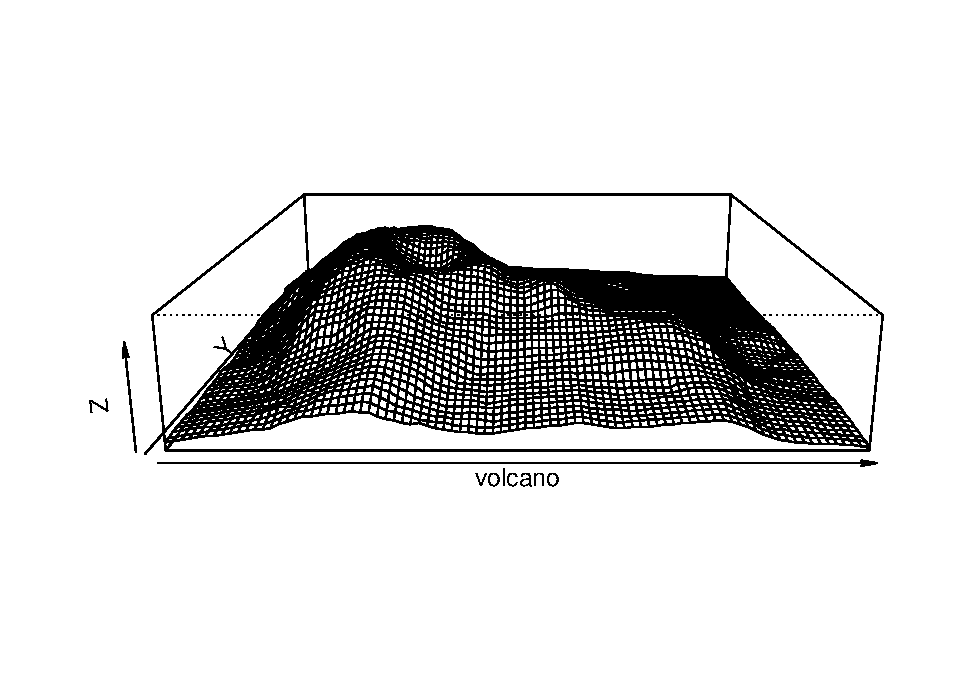
\includegraphics{TudodoR_files/figure-latex/unnamed-chunk-75-1.pdf}

A função \texttt{image} criar um mapa de calor:

\begin{Shaded}
\begin{Highlighting}[]
\KeywordTok{image}\NormalTok{(volcano)}
\end{Highlighting}
\end{Shaded}

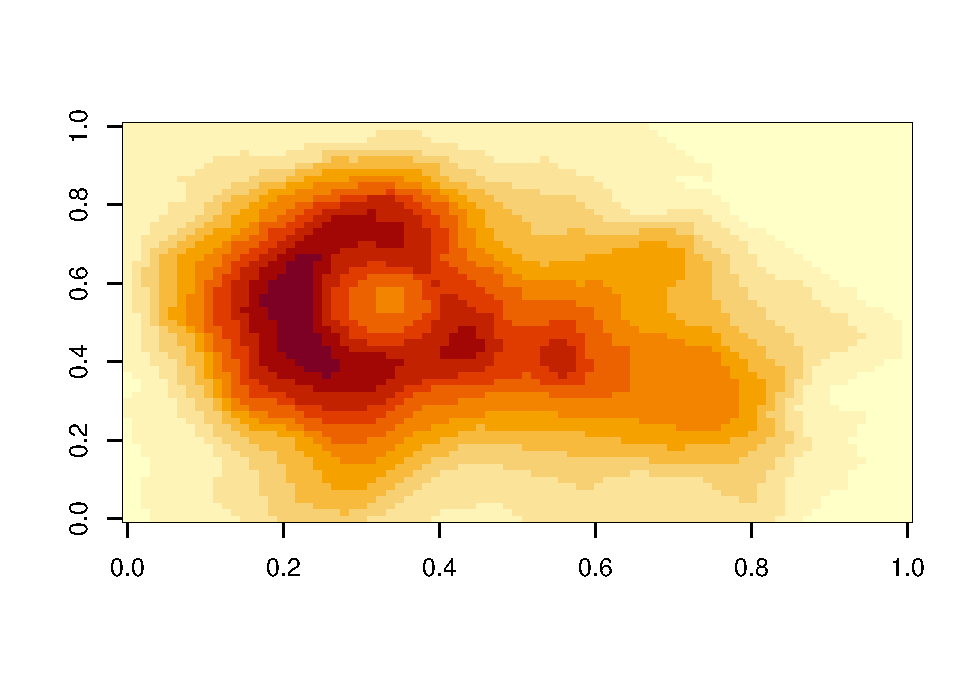
\includegraphics{TudodoR_files/figure-latex/unnamed-chunk-76-1.pdf}

\hypertarget{mais-informacoes-sobre-construcoes-de-matrizes}{%
\subsection{Mais informações sobre construções de Matrizes}\label{mais-informacoes-sobre-construcoes-de-matrizes}}

Há outros comandos que podem ser usados para construir matrizes como \texttt{cbind()} e \texttt{rbind\ ()}. Esses comandos concatenam colunas ou linhas, respectivamente, na matriz (ou vetor).

\begin{Shaded}
\begin{Highlighting}[]
\NormalTok{a <-}\StringTok{ }\KeywordTok{matrix}\NormalTok{ (}\DecValTok{10}\OperatorTok{:}\DecValTok{1}\NormalTok{,}\DataTypeTok{ncol=}\DecValTok{2}\NormalTok{) }\CommentTok{#construir uma matriz qualquer}
\NormalTok{a}
\end{Highlighting}
\end{Shaded}

\begin{verbatim}
##      [,1] [,2]
## [1,]   10    5
## [2,]    9    4
## [3,]    8    3
## [4,]    7    2
## [5,]    6    1
\end{verbatim}

\begin{Shaded}
\begin{Highlighting}[]
\NormalTok{b <-}\StringTok{ }\KeywordTok{cbind}\NormalTok{ (a,}\DecValTok{1}\OperatorTok{:}\DecValTok{5}\NormalTok{) }\CommentTok{#adicionar uma terceira coluna}
\NormalTok{b}
\end{Highlighting}
\end{Shaded}

\begin{verbatim}
##      [,1] [,2] [,3]
## [1,]   10    5    1
## [2,]    9    4    2
## [3,]    8    3    3
## [4,]    7    2    4
## [5,]    6    1    5
\end{verbatim}

\begin{Shaded}
\begin{Highlighting}[]
\NormalTok{c<-}\StringTok{ }\KeywordTok{rbind}\NormalTok{(b,}\KeywordTok{c}\NormalTok{(}\DecValTok{28}\NormalTok{,}\DecValTok{28}\NormalTok{,}\DecValTok{28}\NormalTok{))}
\NormalTok{c}
\end{Highlighting}
\end{Shaded}

\begin{verbatim}
##      [,1] [,2] [,3]
## [1,]   10    5    1
## [2,]    9    4    2
## [3,]    8    3    3
## [4,]    7    2    4
## [5,]    6    1    5
## [6,]   28   28   28
\end{verbatim}

Opcionalmente matrizes podem ter nomes associados ás linhas e colunas (``rownames''e ``colnames''). Cada um destes componentes da matrix é um vetor de nomes.

\begin{Shaded}
\begin{Highlighting}[]
\NormalTok{m1 <-}\StringTok{ }\KeywordTok{matrix}\NormalTok{(}\DecValTok{1}\OperatorTok{:}\DecValTok{12}\NormalTok{, }\DataTypeTok{ncol =} \DecValTok{3}\NormalTok{) }

\KeywordTok{dimnames}\NormalTok{(m1) <-}\StringTok{ }\KeywordTok{list}\NormalTok{(}\KeywordTok{c}\NormalTok{(}\StringTok{"L1"}\NormalTok{, }\StringTok{"L2"}\NormalTok{, }\StringTok{"L3"}\NormalTok{, }\StringTok{"L4"}\NormalTok{), }\KeywordTok{c}\NormalTok{(}\StringTok{"C1"}\NormalTok{, }\StringTok{"C2"}\NormalTok{, }\StringTok{"C3"}\NormalTok{)) }
\KeywordTok{dimnames}\NormalTok{(m1)}
\end{Highlighting}
\end{Shaded}

\begin{verbatim}
## [[1]]
## [1] "L1" "L2" "L3" "L4"
## 
## [[2]]
## [1] "C1" "C2" "C3"
\end{verbatim}

Matrizes são muitas vezes utilizadas para armazenar frequências de cruzamentos entre variáveis. Desta forma é comum surgir a necessidade de obter os totais marginais, isto é a soma dos elementos das linhas e/ou colunas das matrizes, o que pode ser diretamente obtido com \texttt{margin.table(\ )}.

\begin{Shaded}
\begin{Highlighting}[]
 \KeywordTok{margin.table}\NormalTok{(m1, }\DataTypeTok{margin =} \DecValTok{1}\NormalTok{)}
\end{Highlighting}
\end{Shaded}

\begin{verbatim}
## L1 L2 L3 L4 
## 15 18 21 24
\end{verbatim}

\begin{Shaded}
\begin{Highlighting}[]
 \KeywordTok{margin.table}\NormalTok{(m1, }\DataTypeTok{margin =} \DecValTok{2}\NormalTok{)}
\end{Highlighting}
\end{Shaded}

\begin{verbatim}
## C1 C2 C3 
## 10 26 42
\end{verbatim}

\begin{Shaded}
\begin{Highlighting}[]
 \KeywordTok{apply}\NormalTok{(m1, }\DecValTok{2}\NormalTok{, median)}
\end{Highlighting}
\end{Shaded}

\begin{verbatim}
##   C1   C2   C3 
##  2.5  6.5 10.5
\end{verbatim}

\hypertarget{fatores}{%
\section{Fatores}\label{fatores}}

Os fatores são vetores em que os elementos pertencem a uma ou mais categorias temáticas. Por exemplo: ao criar um vetor de indicadores de \textbf{``tratamentos''} em uma análise de experimentos devemos declarar este vetor como um \textbf{``fator''}.
Pode criar um fator usando o comando \textbf{factor()}, ou o comando \textbf{gl}.

\begin{Shaded}
\begin{Highlighting}[]
\KeywordTok{factor}\NormalTok{(}\KeywordTok{rep}\NormalTok{(}\KeywordTok{paste}\NormalTok{(}\StringTok{"T"}\NormalTok{, }\DecValTok{1}\OperatorTok{:}\DecValTok{3}\NormalTok{, }\DataTypeTok{sep =} \StringTok{""}\NormalTok{), }\KeywordTok{c}\NormalTok{(}\DecValTok{4}\NormalTok{, }\DecValTok{4}\NormalTok{, }\DecValTok{3}\NormalTok{)))}
\end{Highlighting}
\end{Shaded}

\begin{verbatim}
##  [1] T1 T1 T1 T1 T2 T2 T2 T2 T3 T3 T3
## Levels: T1 T2 T3
\end{verbatim}

\begin{Shaded}
\begin{Highlighting}[]
\NormalTok{peso  <-}\StringTok{ }\KeywordTok{c}\NormalTok{(}\FloatTok{134.8}\NormalTok{, }\FloatTok{139.7}\NormalTok{, }\FloatTok{147.6}\NormalTok{, }\FloatTok{132.3}\NormalTok{, }\FloatTok{161.7}\NormalTok{, }\FloatTok{157.7}\NormalTok{, }\FloatTok{150.3}\NormalTok{, }\FloatTok{144.7}\NormalTok{,}
           \FloatTok{160.7}\NormalTok{, }\FloatTok{172.7}\NormalTok{, }\FloatTok{163.4}\NormalTok{, }\FloatTok{161.3}\NormalTok{, }\FloatTok{169.8}\NormalTok{, }\FloatTok{168.2}\NormalTok{, }\FloatTok{160.7}\NormalTok{, }\FloatTok{161.0}\NormalTok{,}
           \FloatTok{165.7}\NormalTok{, }\FloatTok{160.0}\NormalTok{, }\FloatTok{158.2}\NormalTok{, }\FloatTok{151.0}\NormalTok{, }\FloatTok{171.8}\NormalTok{, }\FloatTok{157.3}\NormalTok{, }\FloatTok{150.4}\NormalTok{, }\FloatTok{160.4}\NormalTok{,}
           \FloatTok{154.5}\NormalTok{, }\FloatTok{160.4}\NormalTok{, }\FloatTok{148.8}\NormalTok{, }\FloatTok{154.0}\NormalTok{)}
\NormalTok{trat  <-}\StringTok{ }\KeywordTok{rep}\NormalTok{(}\KeywordTok{seq}\NormalTok{(}\DecValTok{0}\NormalTok{,}\DecValTok{300}\NormalTok{,}\DecValTok{50}\NormalTok{), }\DataTypeTok{each=}\DecValTok{4}\NormalTok{)  }\CommentTok{#?each}
\NormalTok{dados <-}\StringTok{  }\KeywordTok{data.frame}\NormalTok{(peso, }\DataTypeTok{trat=}\KeywordTok{as.factor}\NormalTok{(trat))}
\end{Highlighting}
\end{Shaded}

\hypertarget{array}{%
\section{Array}\label{array}}

O conceito de array generaliza a idéia de matrix. Enquanto em uma matrix os elementos são organizados em duas dimensões (linhas e colunas), em um array os elementos podem ser organizados em um número arbitrário de dimensões.
No R um array é definido utilizando a função \texttt{array()}.

\begin{Shaded}
\begin{Highlighting}[]
\NormalTok{ar1 <-}\StringTok{ }\KeywordTok{array}\NormalTok{(}\DecValTok{1}\OperatorTok{:}\DecValTok{24}\NormalTok{, }\DataTypeTok{dim =} \KeywordTok{c}\NormalTok{(}\DecValTok{3}\NormalTok{, }\DecValTok{4}\NormalTok{, }\DecValTok{2}\NormalTok{)) }
\NormalTok{ar1}
\end{Highlighting}
\end{Shaded}

\begin{verbatim}
## , , 1
## 
##      [,1] [,2] [,3] [,4]
## [1,]    1    4    7   10
## [2,]    2    5    8   11
## [3,]    3    6    9   12
## 
## , , 2
## 
##      [,1] [,2] [,3] [,4]
## [1,]   13   16   19   22
## [2,]   14   17   20   23
## [3,]   15   18   21   24
\end{verbatim}

Veja agora um exemplo de dados já incluído no R no formato de array. Para ``carregar'' e visualizar os dados digite:

\begin{Shaded}
\begin{Highlighting}[]
\KeywordTok{data}\NormalTok{(Titanic) }
\NormalTok{Titanic}
\end{Highlighting}
\end{Shaded}

\begin{verbatim}
## , , Age = Child, Survived = No
## 
##       Sex
## Class  Male Female
##   1st     0      0
##   2nd     0      0
##   3rd    35     17
##   Crew    0      0
## 
## , , Age = Adult, Survived = No
## 
##       Sex
## Class  Male Female
##   1st   118      4
##   2nd   154     13
##   3rd   387     89
##   Crew  670      3
## 
## , , Age = Child, Survived = Yes
## 
##       Sex
## Class  Male Female
##   1st     5      1
##   2nd    11     13
##   3rd    13     14
##   Crew    0      0
## 
## , , Age = Adult, Survived = Yes
## 
##       Sex
## Class  Male Female
##   1st    57    140
##   2nd    14     80
##   3rd    75     76
##   Crew  192     20
\end{verbatim}

Para obter maiores informações sobre estes dados digite: \texttt{help(Titanic)}

Agora vamos responder ás seguintes perguntas, mostrando os comandos do R utilizados sobre o array de dados.

\begin{enumerate}
\def\labelenumi{\arabic{enumi}.}
\tightlist
\item
  Quantas pessoas havia no total?
\end{enumerate}

\begin{Shaded}
\begin{Highlighting}[]
\KeywordTok{sum}\NormalTok{(Titanic)}
\end{Highlighting}
\end{Shaded}

\begin{verbatim}
## [1] 2201
\end{verbatim}

\begin{enumerate}
\def\labelenumi{\arabic{enumi}.}
\setcounter{enumi}{1}
\tightlist
\item
  Quantas pessoas havia na tripulação (crew)?
\end{enumerate}

\begin{Shaded}
\begin{Highlighting}[]
\KeywordTok{sum}\NormalTok{(Titanic[}\DecValTok{4}\NormalTok{, , , ])}
\end{Highlighting}
\end{Shaded}

\begin{verbatim}
## [1] 885
\end{verbatim}

\begin{enumerate}
\def\labelenumi{\arabic{enumi}.}
\setcounter{enumi}{2}
\tightlist
\item
  Quantas pessoas sobreviveram e quantas morreram?
\end{enumerate}

\begin{Shaded}
\begin{Highlighting}[]
\KeywordTok{apply}\NormalTok{(Titanic, }\DecValTok{4}\NormalTok{, sum)}
\end{Highlighting}
\end{Shaded}

\begin{verbatim}
##   No  Yes 
## 1490  711
\end{verbatim}

\begin{enumerate}
\def\labelenumi{\arabic{enumi}.}
\setcounter{enumi}{3}
\tightlist
\item
  Quais as proporções de sobreviventes entre homens e mulheres?
\end{enumerate}

\begin{Shaded}
\begin{Highlighting}[]
\KeywordTok{margin.table}\NormalTok{(Titanic, }\DataTypeTok{margin =} \DecValTok{1}\NormalTok{)}
\end{Highlighting}
\end{Shaded}

\begin{verbatim}
## Class
##  1st  2nd  3rd Crew 
##  325  285  706  885
\end{verbatim}

\begin{Shaded}
\begin{Highlighting}[]
\KeywordTok{margin.table}\NormalTok{(Titanic, }\DataTypeTok{margin =} \DecValTok{2}\NormalTok{)}
\end{Highlighting}
\end{Shaded}

\begin{verbatim}
## Sex
##   Male Female 
##   1731    470
\end{verbatim}

\begin{Shaded}
\begin{Highlighting}[]
\KeywordTok{margin.table}\NormalTok{(Titanic, }\DataTypeTok{margin =} \DecValTok{3}\NormalTok{)}
\end{Highlighting}
\end{Shaded}

\begin{verbatim}
## Age
## Child Adult 
##   109  2092
\end{verbatim}

\begin{Shaded}
\begin{Highlighting}[]
\KeywordTok{margin.table}\NormalTok{(Titanic, }\DataTypeTok{margin =} \DecValTok{4}\NormalTok{)}
\end{Highlighting}
\end{Shaded}

\begin{verbatim}
## Survived
##   No  Yes 
## 1490  711
\end{verbatim}

Esta função admite ainda índices múltiplos que permitem outros resumos da tabela de dados. Por exemplo mostramos a seguir como obter o total de sobreviventes e não sobreviventes, separados por sexo e depois as porcentagens de sobreviventes para cada sexo.

\begin{Shaded}
\begin{Highlighting}[]
\KeywordTok{margin.table}\NormalTok{(Titanic, }\DataTypeTok{margin =} \KeywordTok{c}\NormalTok{(}\DecValTok{2}\NormalTok{, }\DecValTok{4}\NormalTok{))}
\end{Highlighting}
\end{Shaded}

\begin{verbatim}
##         Survived
## Sex        No  Yes
##   Male   1364  367
##   Female  126  344
\end{verbatim}

\begin{Shaded}
\begin{Highlighting}[]
\KeywordTok{prop.table}\NormalTok{(}\KeywordTok{margin.table}\NormalTok{(Titanic, }\DataTypeTok{margin =} \KeywordTok{c}\NormalTok{(}\DecValTok{2}\NormalTok{, }\DecValTok{4}\NormalTok{)), }\DataTypeTok{margin =} \DecValTok{1}\NormalTok{)}
\end{Highlighting}
\end{Shaded}

\begin{verbatim}
##         Survived
## Sex             No       Yes
##   Male   0.7879838 0.2120162
##   Female 0.2680851 0.7319149
\end{verbatim}

\begin{Shaded}
\begin{Highlighting}[]
\KeywordTok{prop.table}\NormalTok{(}\KeywordTok{margin.table}\NormalTok{(Titanic, }\DataTypeTok{margin =} \KeywordTok{c}\NormalTok{(}\DecValTok{2}\NormalTok{, }\DecValTok{1}\NormalTok{)), }\DataTypeTok{margin =} \DecValTok{1}\NormalTok{)}
\end{Highlighting}
\end{Shaded}

\begin{verbatim}
##         Class
## Sex             1st        2nd        3rd       Crew
##   Male   0.10398614 0.10340843 0.29462738 0.49797805
##   Female 0.30851064 0.22553191 0.41702128 0.04893617
\end{verbatim}

\hypertarget{data.frame}{%
\section{Data.frame}\label{data.frame}}

Os datas.frames são muitos semelhantes ás matrizes, pois têm linhas e colunas e, portanto, duas dimensões. Entretando, diferentemente das matrizes, colunas diferentes podem armazenar elementos de tipos diferentes. Por exemplo, a primeira coluna pode ser numérica, enquanto a segunda, constituida de caracteres. Cada coluna precisa ter o mesmo tamanho.
Criar o vetor nomes

\begin{Shaded}
\begin{Highlighting}[]
\NormalTok{nome <-}\StringTok{ }\KeywordTok{c}\NormalTok{(}\StringTok{"Melissa José"}\NormalTok{,}
          \StringTok{"Jennifer Linhares"}\NormalTok{,}
          \StringTok{"Gedilene Ponciano"}\NormalTok{,}
          \StringTok{"Edinar da Silva"}\NormalTok{,}
          \StringTok{"Osmar Emidio"}\NormalTok{,}
          \StringTok{"Jeeziel Vieira"}\NormalTok{)}
\end{Highlighting}
\end{Shaded}

Criar vetor idade

\begin{Shaded}
\begin{Highlighting}[]
\NormalTok{idade <-}\StringTok{ }\KeywordTok{c}\NormalTok{(}\DecValTok{17}\NormalTok{,}\DecValTok{18}\NormalTok{,}\DecValTok{16}\NormalTok{,}\DecValTok{15}\NormalTok{,}\DecValTok{15}\NormalTok{,}\DecValTok{18}\NormalTok{)}
\end{Highlighting}
\end{Shaded}

Criar vetor sexo (categoria=fator)

\begin{Shaded}
\begin{Highlighting}[]
\NormalTok{sexo <-}\StringTok{ }\KeywordTok{factor}\NormalTok{(}\KeywordTok{c}\NormalTok{(}\StringTok{"F"}\NormalTok{,}\StringTok{"F"}\NormalTok{,}\StringTok{"F"}\NormalTok{,}\StringTok{"F"}\NormalTok{,}\StringTok{"M"}\NormalTok{,}\StringTok{"M"}\NormalTok{))}
\end{Highlighting}
\end{Shaded}

Criar vetor altura

\begin{Shaded}
\begin{Highlighting}[]
\NormalTok{alt <-}\StringTok{ }\KeywordTok{c}\NormalTok{(}\DecValTok{180}\NormalTok{,}\DecValTok{170}\NormalTok{,}\DecValTok{160}\NormalTok{,}\DecValTok{150}\NormalTok{,}\DecValTok{140}\NormalTok{,}\DecValTok{168}\NormalTok{)}
\end{Highlighting}
\end{Shaded}

Reunir tudo em um data.frame

\begin{Shaded}
\begin{Highlighting}[]
\NormalTok{dados <-}\StringTok{ }\KeywordTok{data.frame}\NormalTok{(nome, idade, sexo, alt)}
\end{Highlighting}
\end{Shaded}

Ver atributos da tabela

\begin{Shaded}
\begin{Highlighting}[]
\KeywordTok{str}\NormalTok{(dados)}
\end{Highlighting}
\end{Shaded}

\begin{verbatim}
## 'data.frame':    6 obs. of  4 variables:
##  $ nome : Factor w/ 6 levels "Edinar da Silva",..: 5 4 2 1 6 3
##  $ idade: num  17 18 16 15 15 18
##  $ sexo : Factor w/ 2 levels "F","M": 1 1 1 1 2 2
##  $ alt  : num  180 170 160 150 140 168
\end{verbatim}

Adicionar nome as linhas com o comando \texttt{row.names()}

\begin{Shaded}
\begin{Highlighting}[]
\KeywordTok{row.names}\NormalTok{(dados) <-}\StringTok{ }\KeywordTok{c}\NormalTok{(}\DecValTok{1}\NormalTok{,}\DecValTok{2}\NormalTok{,}\DecValTok{3}\NormalTok{,}\DecValTok{4}\NormalTok{,}\DecValTok{5}\NormalTok{,}\DecValTok{6}\NormalTok{)}
\NormalTok{dados}
\end{Highlighting}
\end{Shaded}

\begin{verbatim}
##                nome idade sexo alt
## 1      Melissa José    17    F 180
## 2 Jennifer Linhares    18    F 170
## 3 Gedilene Ponciano    16    F 160
## 4   Edinar da Silva    15    F 150
## 5      Osmar Emidio    15    M 140
## 6    Jeeziel Vieira    18    M 168
\end{verbatim}

\begin{Shaded}
\begin{Highlighting}[]
\KeywordTok{names}\NormalTok{(dados) <-}\StringTok{ }\KeywordTok{c}\NormalTok{(}\StringTok{"Nome"}\NormalTok{, }\StringTok{"Idade"}\NormalTok{, }\StringTok{"Sexo"}\NormalTok{, }\StringTok{"altura"}\NormalTok{)}
\NormalTok{dados}
\end{Highlighting}
\end{Shaded}

\begin{verbatim}
##                Nome Idade Sexo altura
## 1      Melissa José    17    F    180
## 2 Jennifer Linhares    18    F    170
## 3 Gedilene Ponciano    16    F    160
## 4   Edinar da Silva    15    F    150
## 5      Osmar Emidio    15    M    140
## 6    Jeeziel Vieira    18    M    168
\end{verbatim}

\hypertarget{indice-dos-data.frames}{%
\subsection{Índice dos Data.frames}\label{indice-dos-data.frames}}

Buscar elementos

\begin{Shaded}
\begin{Highlighting}[]
\NormalTok{dados[}\DecValTok{2}\NormalTok{,}\DecValTok{1}\NormalTok{] }\CommentTok{#elemento da  linha  2, coluna 1}
\end{Highlighting}
\end{Shaded}

\begin{verbatim}
## [1] Jennifer Linhares
## 6 Levels: Edinar da Silva Gedilene Ponciano ... Osmar Emidio
\end{verbatim}

\begin{Shaded}
\begin{Highlighting}[]
\NormalTok{dados[}\DecValTok{2}\NormalTok{,] }\CommentTok{#toda linha dois}
\end{Highlighting}
\end{Shaded}

\begin{verbatim}
##                Nome Idade Sexo altura
## 2 Jennifer Linhares    18    F    170
\end{verbatim}

Repare que apesar de ``Nomes'' ter sido criado como vetor de caracterer o R passou a entender como um fator dentro do data.frame.

\begin{Shaded}
\begin{Highlighting}[]
\NormalTok{dados[,}\DecValTok{1}\NormalTok{]}
\end{Highlighting}
\end{Shaded}

\begin{verbatim}
## [1] Melissa José      Jennifer Linhares Gedilene Ponciano Edinar da Silva  
## [5] Osmar Emidio      Jeeziel Vieira   
## 6 Levels: Edinar da Silva Gedilene Ponciano ... Osmar Emidio
\end{verbatim}

Transformar para caracterer

\begin{Shaded}
\begin{Highlighting}[]
\NormalTok{dados[,}\DecValTok{1}\NormalTok{] <-}\StringTok{ }\KeywordTok{as.character}\NormalTok{(dados[,}\DecValTok{1}\NormalTok{])}
\NormalTok{dados[,}\DecValTok{1}\NormalTok{]}
\end{Highlighting}
\end{Shaded}

\begin{verbatim}
## [1] "Melissa José"      "Jennifer Linhares" "Gedilene Ponciano"
## [4] "Edinar da Silva"   "Osmar Emidio"      "Jeeziel Vieira"
\end{verbatim}

Acessando aos dados

\begin{Shaded}
\begin{Highlighting}[]
\NormalTok{dados}\OperatorTok{$}\NormalTok{Nome}
\end{Highlighting}
\end{Shaded}

\begin{verbatim}
## [1] "Melissa José"      "Jennifer Linhares" "Gedilene Ponciano"
## [4] "Edinar da Silva"   "Osmar Emidio"      "Jeeziel Vieira"
\end{verbatim}

\begin{Shaded}
\begin{Highlighting}[]
\NormalTok{dados}\OperatorTok{$}\NormalTok{Nome[}\DecValTok{3}\NormalTok{]}
\end{Highlighting}
\end{Shaded}

\begin{verbatim}
## [1] "Gedilene Ponciano"
\end{verbatim}

\begin{Shaded}
\begin{Highlighting}[]
\NormalTok{dados}\OperatorTok{$}\NormalTok{Nome [}\DecValTok{1}\OperatorTok{:}\DecValTok{3}\NormalTok{]}
\end{Highlighting}
\end{Shaded}

\begin{verbatim}
## [1] "Melissa José"      "Jennifer Linhares" "Gedilene Ponciano"
\end{verbatim}

\begin{Shaded}
\begin{Highlighting}[]
\KeywordTok{str}\NormalTok{(dados)}
\end{Highlighting}
\end{Shaded}

\begin{verbatim}
## 'data.frame':    6 obs. of  4 variables:
##  $ Nome  : chr  "Melissa José" "Jennifer Linhares" "Gedilene Ponciano" "Edinar da Silva" ...
##  $ Idade : num  17 18 16 15 15 18
##  $ Sexo  : Factor w/ 2 levels "F","M": 1 1 1 1 2 2
##  $ altura: num  180 170 160 150 140 168
\end{verbatim}

\hypertarget{manipulando-um-data.frame}{%
\subsection{Manipulando um Data.frame}\label{manipulando-um-data.frame}}

Você pode manipular um data.frame add ou eliminando colunas ou linhas, assim como em matrizes. Podem-se usar os comandos \texttt{cbind()} e \texttt{rbind\ ()} para adcionar colunas e linhas rescpectivamente, a um data.frame.

\begin{Shaded}
\begin{Highlighting}[]
\NormalTok{dados <-}\StringTok{ }\KeywordTok{cbind}\NormalTok{ (dados, }\CommentTok{#adicionar uma coluna}
               \DataTypeTok{Conceito=}\KeywordTok{c}\NormalTok{(}\StringTok{"A"}\NormalTok{,}\StringTok{"A"}\NormalTok{,}\StringTok{"A"}\NormalTok{,}\StringTok{"C"}\NormalTok{,}\StringTok{"A"}\NormalTok{,}\StringTok{"B"}\NormalTok{))}
\end{Highlighting}
\end{Shaded}

\begin{Shaded}
\begin{Highlighting}[]
\NormalTok{dados <-}\StringTok{ }\KeywordTok{rbind}\NormalTok{ (dados, }\CommentTok{#adicionar uma linha}
                \StringTok{"7"}\NormalTok{=}\StringTok{ }\KeywordTok{c}\NormalTok{(}\StringTok{"Caio Pinto"}\NormalTok{, }\DecValTok{21}\NormalTok{, }\StringTok{"M"}\NormalTok{, }\DecValTok{172}\NormalTok{, }\StringTok{"C"}\NormalTok{))}
\NormalTok{dados}
\end{Highlighting}
\end{Shaded}

\begin{verbatim}
##                Nome Idade Sexo altura Conceito
## 1      Melissa José    17    F    180        A
## 2 Jennifer Linhares    18    F    170        A
## 3 Gedilene Ponciano    16    F    160        A
## 4   Edinar da Silva    15    F    150        C
## 5      Osmar Emidio    15    M    140        A
## 6    Jeeziel Vieira    18    M    168        B
## 7        Caio Pinto    21    M    172        C
\end{verbatim}

Assim como para vetores e matrizes voce pode selecinar um subgrupo de um data.frame e armazena-lo em um outro objeto ou utilizar índices como o sinal negativo para eliminar linhas ou colunas de um data.frame.

\begin{Shaded}
\begin{Highlighting}[]
\NormalTok{dados<-}\StringTok{ }\NormalTok{dados [}\DecValTok{1}\OperatorTok{:}\DecValTok{6}\NormalTok{,] }\CommentTok{#selecionar linha de 1 a 6}
\NormalTok{dados<-}\StringTok{ }\NormalTok{dados [,}\OperatorTok{-}\DecValTok{5}\NormalTok{] }\CommentTok{#excluir a quinta coluna}
\NormalTok{dados}
\end{Highlighting}
\end{Shaded}

\begin{verbatim}
##                Nome Idade Sexo altura
## 1      Melissa José    17    F    180
## 2 Jennifer Linhares    18    F    170
## 3 Gedilene Ponciano    16    F    160
## 4   Edinar da Silva    15    F    150
## 5      Osmar Emidio    15    M    140
## 6    Jeeziel Vieira    18    M    168
\end{verbatim}

\begin{Shaded}
\begin{Highlighting}[]
\NormalTok{dados[dados}\OperatorTok{$}\NormalTok{Sexo}\OperatorTok{==}\StringTok{"F"}\NormalTok{,] }\CommentTok{#exibir só masculinos}
\end{Highlighting}
\end{Shaded}

\begin{verbatim}
##                Nome Idade Sexo altura
## 1      Melissa José    17    F    180
## 2 Jennifer Linhares    18    F    170
## 3 Gedilene Ponciano    16    F    160
## 4   Edinar da Silva    15    F    150
\end{verbatim}

A ordenação das linhas de um \textbf{data.frame} segundo os dados contidos em determinadas coluna também é extremamente útil

\begin{Shaded}
\begin{Highlighting}[]
\NormalTok{dados [}\KeywordTok{order}\NormalTok{(dados}\OperatorTok{$}\NormalTok{altura),]}
\end{Highlighting}
\end{Shaded}

\begin{verbatim}
##                Nome Idade Sexo altura
## 5      Osmar Emidio    15    M    140
## 4   Edinar da Silva    15    F    150
## 3 Gedilene Ponciano    16    F    160
## 6    Jeeziel Vieira    18    M    168
## 2 Jennifer Linhares    18    F    170
## 1      Melissa José    17    F    180
\end{verbatim}

\begin{Shaded}
\begin{Highlighting}[]
\NormalTok{dados [}\KeywordTok{rev}\NormalTok{(}\KeywordTok{order}\NormalTok{(dados}\OperatorTok{$}\NormalTok{altura)),]}
\end{Highlighting}
\end{Shaded}

\begin{verbatim}
##                Nome Idade Sexo altura
## 1      Melissa José    17    F    180
## 2 Jennifer Linhares    18    F    170
## 6    Jeeziel Vieira    18    M    168
## 3 Gedilene Ponciano    16    F    160
## 4   Edinar da Silva    15    F    150
## 5      Osmar Emidio    15    M    140
\end{verbatim}

\hypertarget{separando-um-data.frame-por-grupos}{%
\subsection{Separando um data.frame por grupos}\label{separando-um-data.frame-por-grupos}}

\begin{Shaded}
\begin{Highlighting}[]
\KeywordTok{split}\NormalTok{ (dados, sexo)}
\end{Highlighting}
\end{Shaded}

\begin{verbatim}
## $F
##                Nome Idade Sexo altura
## 1      Melissa José    17    F    180
## 2 Jennifer Linhares    18    F    170
## 3 Gedilene Ponciano    16    F    160
## 4   Edinar da Silva    15    F    150
## 
## $M
##             Nome Idade Sexo altura
## 5   Osmar Emidio    15    M    140
## 6 Jeeziel Vieira    18    M    168
\end{verbatim}

\hypertarget{lista}{%
\section{Lista}\label{lista}}

Lista são objetos muito úteis, pois são usados para combinar diferente estruturas de dados em um mesmo objeto, ou seja, vetores, matrizes, arrays, data.frames e ate mesmo outras listas.

\begin{Shaded}
\begin{Highlighting}[]
\NormalTok{pes <-}\StringTok{ }\KeywordTok{list}\NormalTok{ (}\DataTypeTok{idade=}\DecValTok{32}\NormalTok{, }\DataTypeTok{nome=}\StringTok{"Maria"}\NormalTok{, }\DataTypeTok{notas=}\KeywordTok{c}\NormalTok{(}\DecValTok{98}\NormalTok{,}\DecValTok{95}\NormalTok{,}\DecValTok{78}\NormalTok{), }\DataTypeTok{B=}\KeywordTok{matrix}\NormalTok{(}\DecValTok{1}\OperatorTok{:}\DecValTok{4}\NormalTok{,}\DecValTok{2}\NormalTok{,}\DecValTok{2}\NormalTok{))}
\NormalTok{pes}
\end{Highlighting}
\end{Shaded}

\begin{verbatim}
## $idade
## [1] 32
## 
## $nome
## [1] "Maria"
## 
## $notas
## [1] 98 95 78
## 
## $B
##      [,1] [,2]
## [1,]    1    3
## [2,]    2    4
\end{verbatim}

Lista são construidas com o comando \texttt{list\ ()}. Quando você exibe um objeto que é uma lista, cada componente é mostrado com seu nome \textbf{\$} ou \textbf{{[} {]}}

\hypertarget{alguns-comandos-que-retornam-listas}{%
\subsection{Alguns comandos que retornam listas}\label{alguns-comandos-que-retornam-listas}}

Muitos comando do R retornam seu resultado na forma de listas. Um exemplo pode ser mostrado com o uso do comando \texttt{t.tes()}, que retorna um objeto que é uma lista.

\begin{Shaded}
\begin{Highlighting}[]
\NormalTok{x <-}\StringTok{ }\KeywordTok{c}\NormalTok{(}\DecValTok{1}\NormalTok{,}\DecValTok{3}\NormalTok{,}\DecValTok{2}\NormalTok{,}\DecValTok{3}\NormalTok{,}\DecValTok{4}\NormalTok{)}
\NormalTok{y <-}\StringTok{ }\KeywordTok{c}\NormalTok{(}\DecValTok{4}\NormalTok{,}\DecValTok{5}\NormalTok{,}\DecValTok{5}\NormalTok{,}\DecValTok{4}\NormalTok{,}\DecValTok{4}\NormalTok{)}
\NormalTok{tt <-}\StringTok{ }\KeywordTok{t.test}\NormalTok{ (x,y, }\DataTypeTok{var.equal=}\NormalTok{T)}
\NormalTok{tt}
\end{Highlighting}
\end{Shaded}

\begin{verbatim}
## 
##  Two Sample t-test
## 
## data:  x and y
## t = -3.182, df = 8, p-value = 0.01296
## alternative hypothesis: true difference in means is not equal to 0
## 95 percent confidence interval:
##  -3.1044729 -0.4955271
## sample estimates:
## mean of x mean of y 
##       2.6       4.4
\end{verbatim}

Comprovar que é uma lista

\begin{Shaded}
\begin{Highlighting}[]
\KeywordTok{is.list}\NormalTok{(tt)}
\end{Highlighting}
\end{Shaded}

\begin{verbatim}
## [1] TRUE
\end{verbatim}

\begin{Shaded}
\begin{Highlighting}[]
\KeywordTok{mode}\NormalTok{ (tt)}
\end{Highlighting}
\end{Shaded}

\begin{verbatim}
## [1] "list"
\end{verbatim}

Exibir o componentes da lista

\begin{Shaded}
\begin{Highlighting}[]
\KeywordTok{names}\NormalTok{(tt)}
\end{Highlighting}
\end{Shaded}

\begin{verbatim}
##  [1] "statistic"   "parameter"   "p.value"     "conf.int"    "estimate"   
##  [6] "null.value"  "stderr"      "alternative" "method"      "data.name"
\end{verbatim}

\begin{Shaded}
\begin{Highlighting}[]
\NormalTok{tt}\OperatorTok{$}\NormalTok{conf.int }\CommentTok{#intervalo de confianca }
\end{Highlighting}
\end{Shaded}

\begin{verbatim}
## [1] -3.1044729 -0.4955271
## attr(,"conf.level")
## [1] 0.95
\end{verbatim}

\hypertarget{referencia-1}{%
\section{Referência}\label{referencia-1}}

MELO, M. P.; PETERNELI, L. A. \textbf{Conhecendo o R: Um visão mais que estatística}. Viçosa, MG: UFV, 2013. 222p.

\textbf{Prof.~Paulo Justiniando Ribeiro} \textgreater{}\url{http://www.leg.ufpr.br/~paulojus/}\textless{}

\textbf{Prof.~Adriano Azevedo Filho} \textgreater{}\url{http://rpubs.com/adriano/esalq2012inicial}\textless{}

\textbf{Prof.~Fernando de Pol Mayer} \textgreater{}\url{https://fernandomayer.github.io/ce083-2016-2/}\textless{}

\textbf{Site Interativo Datacamp} \textgreater{}\url{https://www.datacamp.com/}\textless{}

\hypertarget{entrada-de-dados}{%
\chapter{Entrada de dados}\label{entrada-de-dados}}

Este terceiro Capitulo foi baseado no livro \href{https://www.editoraufv.com.br/produto/conhecendo-o-r-uma-visao-mais-que-estatistica/1109294}{\textbf{Conhecendo o R: Um visão mais que estatística}}, e na página do \href{http://www.leg.ufpr.br/~paulojus/}{\textbf{Prof.~Paulo Justiniando Ribeiro}} modificações foram realizadas utilizando outros materiais que se encontram referenciado no final do Capitulo.

O diretorio de trabalho é aquele usado pelo R para gravar, ler, importar e exportar arquivos quando nenhum outro caminho é explicitado.

\hypertarget{onde-os-dados-devem-estar}{%
\section{Onde os dados devem estar?}\label{onde-os-dados-devem-estar}}

Para saber onde os diretorios estão basta digitar o comando \texttt{getwd()}

\begin{Shaded}
\begin{Highlighting}[]
 \KeywordTok{getwd}\NormalTok{() }\CommentTok{#para verificar  diretório de trabalho}
\end{Highlighting}
\end{Shaded}

\begin{verbatim}
## [1] "D:/livro/TudodoRa"
\end{verbatim}

Caso queira alterar o diretorio de trabalho para um outro qualquer digite o comando \texttt{setwd()}

\begin{Shaded}
\begin{Highlighting}[]
\KeywordTok{setwd}\NormalTok{(}\StringTok{"C:/R_Curso"}\NormalTok{) }\CommentTok{#para  altear o diretório de trabalho}
\end{Highlighting}
\end{Shaded}

Outra forma de mudar o caminho é com o comando:

\begin{Shaded}
\begin{Highlighting}[]
\NormalTok{caminho<-}\KeywordTok{file.choose}\NormalTok{() }\CommentTok{# ou usando as teclhas shift + Crtl + H}
\end{Highlighting}
\end{Shaded}

Este comando irá abrir uma tela para que o usuário navegue nas pastas e escolha o arquivo a ser aberto.

Você pode exibir o conteudo do diretório com o comando \texttt{dir()}

\begin{Shaded}
\begin{Highlighting}[]
\KeywordTok{dir}\NormalTok{()}
\end{Highlighting}
\end{Shaded}

\begin{verbatim}
##  [1] "_bookdown.yml"     "_bookdown_files"   "_output.yml"      
##  [4] "01-intro.Rmd"      "02-literature.Rmd" "04-Estrutura.Rmd" 
##  [7] "05-Figura.Rmd"     "06-references.Rmd" "book.bib"         
## [10] "docs"              "index.Rmd"         "LICENSE"          
## [13] "meu grafico.bmp"   "meu grafico.jpg"   "meu grafico.png"  
## [16] "meu grafico.ps"    "meu grafico.wmf"   "meugráfico.pdf"   
## [19] "packages.bib"      "preamble.tex"      "README.md"        
## [22] "search_index.json" "style.css"         "TudodoR.log"      
## [25] "TudodoR.pdf"       "TudodoR.Rmd"       "TudodoR.Rproj"    
## [28] "TudodoR.tex"       "TudodoR_files"
\end{verbatim}

\hypertarget{entrando-com-dados}{%
\section{Entrando com dados}\label{entrando-com-dados}}

O formato mais adequado vai depender do tamanho do conjunto de dados, e se os dados já existem em outro formato para serem importados ou se serão digitados diretamente no R.

A seguir são descritas formas de entrada de dados com indicão de quando cada uma das formas deve ser usada.

\hypertarget{vetores}{%
\subsection{Vetores}\label{vetores}}

Podemos entrar com dados definindo vetores com o comando \texttt{c()}, conforme visto no capítulo 3.

\begin{Shaded}
\begin{Highlighting}[]
\NormalTok{vetor <-}\StringTok{ }\KeywordTok{c}\NormalTok{(}\DecValTok{2}\NormalTok{,}\DecValTok{5}\NormalTok{,}\DecValTok{7}\NormalTok{)}
\end{Highlighting}
\end{Shaded}

Esta forma de entrada de dados é conveniente quando se tem um pequeno número de dados. Quando os dados tem algum elementos repetidos, números sequenciais pode-se usar mecanismos do R para facilitar a entrada dos dados como vetores.

\begin{Shaded}
\begin{Highlighting}[]
\NormalTok{vetor <-}\StringTok{ }\KeywordTok{rep}\NormalTok{(}\KeywordTok{c}\NormalTok{(}\DecValTok{2}\NormalTok{,}\DecValTok{5}\NormalTok{), }\DecValTok{5}\NormalTok{)  }\CommentTok{# cria vetor repetindo 5 vezes 2 e 5 alternadamente}
\NormalTok{vetor}
\end{Highlighting}
\end{Shaded}

\begin{verbatim}
##  [1] 2 5 2 5 2 5 2 5 2 5
\end{verbatim}

\begin{Shaded}
\begin{Highlighting}[]
\NormalTok{vetor <-}\StringTok{ }\KeywordTok{rep}\NormalTok{(}\KeywordTok{c}\NormalTok{(}\DecValTok{5}\NormalTok{,}\DecValTok{8}\NormalTok{), }\DataTypeTok{each=}\DecValTok{3}\NormalTok{)  }\CommentTok{# cria vetor repetindo 3 vezes 5 e depois 8}
\NormalTok{vetor}
\end{Highlighting}
\end{Shaded}

\begin{verbatim}
## [1] 5 5 5 8 8 8
\end{verbatim}

\hypertarget{usando-a-funcao-scan}{%
\subsection{Usando a função `scan'}\label{usando-a-funcao-scan}}

Esta função coloca o modo prompt onde o usuário deve digitar cada dado seguido da tecla . Para encerrar a entrada de dados basta digitar duas vezes consecutivas. Veja o seguinte resultado:

\begin{Shaded}
\begin{Highlighting}[]
\NormalTok{y <-}\StringTok{ }\KeywordTok{scan}\NormalTok{()}

\CommentTok{#1: 11}
\CommentTok{#2: 24}
\CommentTok{#3: 35}
\CommentTok{#4: 29}
\CommentTok{#5: 39}
\CommentTok{#6: 47}
\CommentTok{#7:}
\CommentTok{#Read 6 items}

\NormalTok{y}
\end{Highlighting}
\end{Shaded}

\begin{verbatim}
## numeric(0)
\end{verbatim}

\begin{Shaded}
\begin{Highlighting}[]
\CommentTok{#[1] 11 24 35 29 39 47}
\end{Highlighting}
\end{Shaded}

Este formato é mais ágil que o anterior e mais conveniente para digitar vetores longos.

\hypertarget{copiar-e-colar-usando-scan}{%
\subsection{Copiar e colar usando scan()}\label{copiar-e-colar-usando-scan}}

Pode usar o recurso ``copiar e colar'' com o comando \texttt{scan}.
Após copiar os dados (crtl+C), digite no \textbf{prompt}/\textbf{console} o comando \texttt{scan()}, aperte \textgreater ENTER\textless, depois cole o texto e, aperte \textgreater ENTER\textless{} novamente.

\hypertarget{lendo-dados-atraves-da-area-de-transferencia}{%
\subsection{Lendo dados através da área de transferência}\label{lendo-dados-atraves-da-area-de-transferencia}}

Funções como \texttt{scan()}, \texttt{read.table()} e outras podem usadas para ler os dados diretamente da área de transferência passando-se ao \emph{``clipboard''} ao primeiro argumento.

\hypertarget{usando-a-funcao-edit}{%
\subsection{Usando a função edit}\label{usando-a-funcao-edit}}

O comando \texttt{edit(data.frame())} abre uma planilha para digitação de dados que são armazanados como data-frames.

\begin{Shaded}
\begin{Highlighting}[]
\NormalTok{dados <-}\StringTok{ }\KeywordTok{edit}\NormalTok{(}\KeywordTok{data.frame}\NormalTok{())}
\end{Highlighting}
\end{Shaded}

\begin{figure}
\centering
\includegraphics{https://www.dropbox.com/s/cbsqhtze2715m8t/scan1.PNG?dl=1}
\caption{data-frame}
\end{figure}

Se voce precisar abrir novamente planilha com os dados, para fazer modificações e/ou inserir mais dados use o comando \texttt{fix}.

\begin{Shaded}
\begin{Highlighting}[]
\KeywordTok{fix}\NormalTok{(dados)}
\KeywordTok{head}\NormalTok{(dados)}
\end{Highlighting}
\end{Shaded}

\begin{verbatim}
## data frame with 0 columns and 0 rows
\end{verbatim}

\hypertarget{exemplo-1}{%
\subsubsection{Exemplo 1}\label{exemplo-1}}

\begin{Shaded}
\begin{Highlighting}[]
\NormalTok{teste <-}\StringTok{ }\KeywordTok{c}\NormalTok{(}\DecValTok{10}\NormalTok{,}\DecValTok{20}\NormalTok{,}\DecValTok{30}\NormalTok{,}\DecValTok{40}\NormalTok{,}\DecValTok{50}\NormalTok{)}
\NormalTok{teste}
\end{Highlighting}
\end{Shaded}

\begin{verbatim}
## [1] 10 20 30 40 50
\end{verbatim}

Porém houve um erro: o último elemento deveria ser 60 e não 50, você não precisar criar novamente um objeto, use o comando \texttt{edit()}

\begin{Shaded}
\begin{Highlighting}[]
\NormalTok{teste2 <-}\StringTok{ }\KeywordTok{edit}\NormalTok{(teste)}
\end{Highlighting}
\end{Shaded}

\begin{figure}
\centering
\includegraphics{https://www.dropbox.com/s/l6eh9s5f46wr71x/edit2.PNG?dl=1}
\caption{edit}
\end{figure}

\hypertarget{exemplo-2}{%
\subsubsection{Exemplo 2}\label{exemplo-2}}

Com uma planilha com três colunas de dados. Os valores numéricos da coluna poderiam ser importados para o R utilizando-se o mesmo processo ora descrito com o uso do comando \texttt{scan()}. Abra o arquivo . \href{https://www.dropbox.com/s/6504oo4olw34dw9/EVI_Prec.xlsx?dl=1}{EVI-prec.xlsx}.

Uma matrix com os dados poderá ser obtida com o comando \texttt{cbind}

\begin{Shaded}
\begin{Highlighting}[]
\NormalTok{dados <-}\StringTok{ }\KeywordTok{cbind}\NormalTok{(ano, chuva, evi)}
\end{Highlighting}
\end{Shaded}

Os objeto dados é um \textbf{data.frame}

\begin{Shaded}
\begin{Highlighting}[]
\KeywordTok{is.data.frame}\NormalTok{(dados)}
\end{Highlighting}
\end{Shaded}

Transforme para um data.frame com o comando \textbf{as.data.frame}

\begin{Shaded}
\begin{Highlighting}[]
\NormalTok{dados_m <-}\StringTok{ }\KeywordTok{as.data.frame}\NormalTok{(dados)}
\end{Highlighting}
\end{Shaded}

Poderia usar o comando data.frame direto

\begin{Shaded}
\begin{Highlighting}[]
\NormalTok{dados=}\KeywordTok{data.frame}\NormalTok{ (ano, chuva, evi)}
\end{Highlighting}
\end{Shaded}

\hypertarget{lendo-dados-de-um-arquivo-texto}{%
\subsection{Lendo dados de um arquivo texto}\label{lendo-dados-de-um-arquivo-texto}}

É muito importante ter os dados tabulados em um arquivo-texto ou em outros formatos que permitem a conversão para dados texto. O comando \texttt{read.table\ ()} é extremamente útil por ler dados de um arquivo-texto no formato de um \textbf{data.frame}

Usando o Comando \texttt{read.table\ ()}

\hypertarget{exemplo-1-1}{%
\subsubsection{Exemplo 1}\label{exemplo-1-1}}

Como primeiro exemplo considere importar para o R os dados do arquivo texto \href{https://www.dropbox.com/s/m7jivbbggei5y0x/exemplo1.txt?dl=1}{exemplo1.txt}.

\begin{Shaded}
\begin{Highlighting}[]
\NormalTok{ex01 <-}\StringTok{ }\KeywordTok{read.table}\NormalTok{(}\StringTok{"exemplo1.txt"}\NormalTok{) }

\CommentTok{#Use os comandos}
\NormalTok{  ex01}
  \KeywordTok{class}\NormalTok{(ex01)}
  \KeywordTok{names}\NormalTok{(ex01)}
  \KeywordTok{dim}\NormalTok{(ex01)}
  \KeywordTok{str}\NormalTok{(ex01)}
  \KeywordTok{head}\NormalTok{(ex01)}
\end{Highlighting}
\end{Shaded}

\hypertarget{exemplo-2-1}{%
\subsubsection{Exemplo 2}\label{exemplo-2-1}}

Como primeiro exemplo considere importar para o R os dados do arquivo de texto \href{https://www.dropbox.com/s/bi4b0j2nnnetc1r/exemplo2.txt?dl=1}{exemplo2.txt}.

\begin{Shaded}
\begin{Highlighting}[]
\NormalTok{ex02 <-}\StringTok{ }\KeywordTok{read.table}\NormalTok{(}\StringTok{"exemplo2.txt"}\NormalTok{) }
\NormalTok{ex02}
\end{Highlighting}
\end{Shaded}

Note que este arquivo difere do anterior em um aspecto: os nomes das variáveis estão na primeira linha. Para que o R considere isto corretamente temos que informá-lo disto com o argumento \emph{head=T}. Portanto para importar este arquivo usamos:

\begin{Shaded}
\begin{Highlighting}[]
\NormalTok{ex02 <-}\StringTok{ }\KeywordTok{read.table}\NormalTok{(}\StringTok{"exemplo02.txt"}\NormalTok{, }\DataTypeTok{head=}\NormalTok{T) }
\NormalTok{ex02}
\end{Highlighting}
\end{Shaded}

\hypertarget{dados-do-tipo-csv}{%
\subsection{Dados do tipo CSV}\label{dados-do-tipo-csv}}

\href{https://www.dropbox.com/s/mv13cmkysw2nizm/exemplo3.csv?dl=1}{Exemplo3.csv}: Vamos utilizar um arquivo de tipo \textbf{CSV}.

\begin{Shaded}
\begin{Highlighting}[]
\NormalTok{ex03 <-}\StringTok{ }\KeywordTok{read.table}\NormalTok{(}\StringTok{"exemplo3.csv."}\NormalTok{, }\DataTypeTok{head=}\NormalTok{T, }\DataTypeTok{sep=}\StringTok{":"}\NormalTok{, }\DataTypeTok{dec=}\StringTok{","}\NormalTok{) }
\NormalTok{ex03}
\end{Highlighting}
\end{Shaded}

Note que este arquivo difere do primeiro em outros aspectos.
\emph{read.table.}

\begin{Shaded}
\begin{Highlighting}[]
\NormalTok{ex03 <-}\StringTok{ }\KeywordTok{read.table}\NormalTok{(       }\CommentTok{# lê dados de um arquivo texto}
  \StringTok{"exemplo3.csv"}\NormalTok{,         }\CommentTok{# nome do arquivo ou o caminho c:/R.exemplo3.csv}
  \DataTypeTok{head=}\NormalTok{T,                 }\CommentTok{# primeira linha ? cabe?alho}
  \DataTypeTok{sep=}\StringTok{":"}\NormalTok{,                }\CommentTok{# separador de coluna }
  \DataTypeTok{dec=}\StringTok{","}\NormalTok{)                }\CommentTok{# virgula como separador}
\NormalTok{ex03                      }\CommentTok{# exibe o objeto}
\end{Highlighting}
\end{Shaded}

1.\textbf{sep}: caractere utilizado para separação dos campos e valores. Normalmente é utilizado o ponto e virgula (;)

1.\textbf{dec}: caractere utilizado para separar as casas decimais. Normalmente ponto (.) ou virgula (,).

1.\textbf{header}: TRUE, assume que a primeira linha da tabela contêm rotulos das variáveis. `FALSE', assume que os dados se iniciam na primeira linha.

\hypertarget{a-seguir-listamos-algumas-destas-funcoes}{%
\subsection{A seguir listamos algumas destas funções:}\label{a-seguir-listamos-algumas-destas-funcoes}}

\begin{enumerate}
\def\labelenumi{\arabic{enumi}.}
\tightlist
\item
  \emph{read.dbf()} para arquivos DBASE
\item
  \emph{read.epiinfo()} para arquivos .REC do Epi-Info
\item
  \emph{read.mtp()} para arquivos ``Minitab Portable Worksheet''
\item
  \emph{read.S()} para arquivos do S-PLUS, e restore.data() para ``dumps'' do S-PLUS
\item
  \emph{read.spss()} para dados do SPSS
\item
  \emph{read.systat()} para dados do SYSTAT
\item
  \emph{read.dta()} para dados do STATA
\item
  \emph{read.octave()} para dados do OCTAVE (um clone do MATLAB)
\item
  \emph{read.csv}(file, header = TRUE, sep=``,'', dec=``.'')
\item
  \emph{read.csv2}(file, header = TRUE, sep=``;'', dec=``,'')
\item
  \emph{read.delim}(file, header = TRUE, sep=``\t", dec=''.")
\item
  \emph{read.delim2}(file, header = TRUE, sep=``\t", dec='',")
\end{enumerate}

\hypertarget{lendo-dados-disponiveis-na-web}{%
\subsection{Lendo dados disponíveis na web}\label{lendo-dados-disponiveis-na-web}}

\textbf{Exemplo 4}: As funções permitem ler ainda dados diretamente disponíveis na web. Por exemplo os dados do \href{https://www.dropbox.com/s/m7jivbbggei5y0x/exemplo1.txt?dl=1}{exemplo1.txt} poderiam ser lidos diretamente com o comando a seguir

\hypertarget{lendo-dados-de-uma-planilha-eletronica}{%
\subsection{Lendo dados de uma planilha eletrônica}\label{lendo-dados-de-uma-planilha-eletronica}}

Com o \textbf{pacote xlsx} é possivel ler os dados diretamente da planilha eletrônica do Excel.

\begin{Shaded}
\begin{Highlighting}[]
\KeywordTok{install.packages}\NormalTok{(}\StringTok{""}\NormalTok{)}
\KeywordTok{require}\NormalTok{(}\StringTok{"xlsx"}\NormalTok{)}
\end{Highlighting}
\end{Shaded}

O comando \emph{read.xlsx()}, do \textbf{pacote xlsx}, lê o conteúdo de uma planilha eletrônica para o R com a estrutura de dados de um \emph{data.frame}.

\begin{Shaded}
\begin{Highlighting}[]
\NormalTok{dados <-}\StringTok{ }\KeywordTok{read.xlsx}\NormalTok{(}
                    \DataTypeTok{file=}\StringTok{"C:/R/EVI_Prec.xlsx"}\NormalTok{,     }\CommentTok{#comando que lê planilhas}
                    \DataTypeTok{sheetName =} \StringTok{"Conbea"}\NormalTok{,          }\CommentTok{#nome da planilha}
                    \DataTypeTok{h=}\NormalTok{T)                           }\CommentTok{#sem cabeçalho  }
\end{Highlighting}
\end{Shaded}

\hypertarget{exercicios}{%
\subsection{Exercícios}\label{exercicios}}

\begin{enumerate}
\def\labelenumi{\arabic{enumi}.}
\tightlist
\item
  Baixe os seguintes arquivos:

  \begin{itemize}
  \tightlist
  \item
    \href{https://www.dropbox.com/s/uq1n2sv8an2eoan/BanzattoQd1.2.3.txt?dl=1}{BanzattoQd1.2.3.txt}
  \item
    \href{https://www.dropbox.com/s/jjyo8dhyy0qt3ft/BanzattoQd3.2.1.txt?dl=1}{BanzattoQd3.2.1.txt}
  \item
    \href{https://www.dropbox.com/s/yv5clm6qljurzbw/BanzattoQd3.4.1.txt?dl=1}{BanzattoQd3.4.1.txt}
  \end{itemize}
\end{enumerate}

Coloque os arquivos em um local apropriado (de preferncia no mesmo diretorio de trabalho que voce definiu no início da sessão), faça a importação usando a função de sua escolha, e confira a estrutura dos dados com ´str()´.

\hypertarget{salvar-objetos-de-dados}{%
\section{Salvar objetos de dados}\label{salvar-objetos-de-dados}}

Salvar objetos de dados nos formatos \textbf{.txt} ou \textbf{.csv}
função: \textbf{write.table}
sintaxe da função:
\emph{write.table}(x, file, sep="``, dec=''", rownames = T, col.names = T)

Principais argumentos:
1. x - matriz ou data frame
1. file - nome do arquivo ou caminho do arquivo
1. sep - separador da coluna
1. dec - separador deciminal

\hypertarget{outras-funcoes}{%
\subsection{Outras funções}\label{outras-funcoes}}

\texttt{write.csv()}
\texttt{write.csv2()}
\texttt{write.xlsx\ ()}

\textbf{Exemplo:}
write.xlsx(dados,``tabela salva.xlsx'')

\hypertarget{referencia-2}{%
\section{Referência}\label{referencia-2}}

MELO, M. P.; PETERNELI, L. A. \textbf{Conhecendo o R: Um visão mais que estatística}. Viçosa, MG: UFV, 2013. 222p.

\textbf{Prof.~Paulo Justiniando Ribeiro} \textgreater{}\url{http://www.leg.ufpr.br/~paulojus/}\textless{}

\textbf{Prof.~Adriano Azevedo Filho} \textgreater{}\url{http://rpubs.com/adriano/esalq2012inicial}\textless{}

\textbf{Prof.~Fernando de Pol Mayer} \textgreater{}\url{https://fernandomayer.github.io/ce083-2016-2/}\textless{}

\hypertarget{criando-graficos-com-o-r}{%
\chapter{Criando Gráficos com o R}\label{criando-graficos-com-o-r}}

Este capitulo foi baseado nos livros

\begin{itemize}
\item
  \href{https://www.editoraufv.com.br/produto/conhecendo-o-r-uma-visao-mais-que-estatistica/1109294}{\textbf{Conhecendo o R: Um visão mais que estatística}}
\item
  AQUINO, J. A. \textbf{R para cientistas sociais}. - Ilhéus, BA: EDITUS, 2014. 157.
\item
  ANJOS, A. \textbf{Análise gráfica com uso do R}. Apostila. Dep. de Estatistica da UFPR, 2016. 127p.
\end{itemize}

Sites

\begin{itemize}
\item
  \url{https://www.statmethods.net/index.html}
\item
  \url{http://curso-r.github.io/index.html} PET Estatística UFPR (2016). \textbf{labestData: Biblioteca de Dados para Aprendizado de Estatística}. R package version x.y-z.w.
\item
  \url{https://www.statmethods.net/index.html}
\end{itemize}

Modificações foram realizadas utilizando outros materiais que se encontram referenciado no final do Capitulo.

O R é uma poderosa ferramenta no que diz respeito à confeção de gráficos. Iremos abordar três categorias de comandos gráficos, com o uso do pacote báscico do R o \emph{graphics". Alguns pacotes foram desenvolvidos especialmente para manipulação de gráficos, como
}lattice\emph{, }ggplot2\emph{, }ggobi* e \emph{rgl}.

O R possui diferentes funções geradoras de gráficos, e essas são classificados como:

\begin{itemize}
\item
  \emph{Funções gráficas de alto nível}: criam novos gráficos na janela, definindo eixos, título, etc. Exemplos: \emph{plot, hist, image, contour, persp etc}.
\item
  \emph{Funções gráficas de baixo nível}: permitem adicionar novas informações em gráficos já criados, como novos dados, linhas etc. Exemplos: \emph{points, lines, abline,} \emph{polygon, legend etc}.
\item
  \emph{Funções gráficas iterativas}: permitem retirar ou adicionar informações aos gráficos já existentes, usando por exemplo o cursor do mouse. Exemplos: \emph{locator e identify}.
\end{itemize}

\hypertarget{exemplos-de-graficos-com-o-r}{%
\section{Exemplos de gráficos com o R}\label{exemplos-de-graficos-com-o-r}}

Você pode ver alguns exemplos de gráficos que podem ser criados no R com os seguintes comandos:

\begin{Shaded}
\begin{Highlighting}[]
\KeywordTok{demo}\NormalTok{(image)}
\end{Highlighting}
\end{Shaded}

\begin{verbatim}
## 
## 
##  demo(image)
##  ---- ~~~~~
## 
## > #  Copyright (C) 1997-2009 The R Core Team
## > 
## > require(datasets)
## 
## > require(grDevices); require(graphics)
## 
## > x <- 10*(1:nrow(volcano)); x.at <- seq(100, 800, by=100)
## 
## > y <- 10*(1:ncol(volcano)); y.at <- seq(100, 600, by=100)
## 
## >                    # Using Terrain Colors
## > 
## > image(x, y, volcano, col=terrain.colors(100),axes=FALSE)
\end{verbatim}

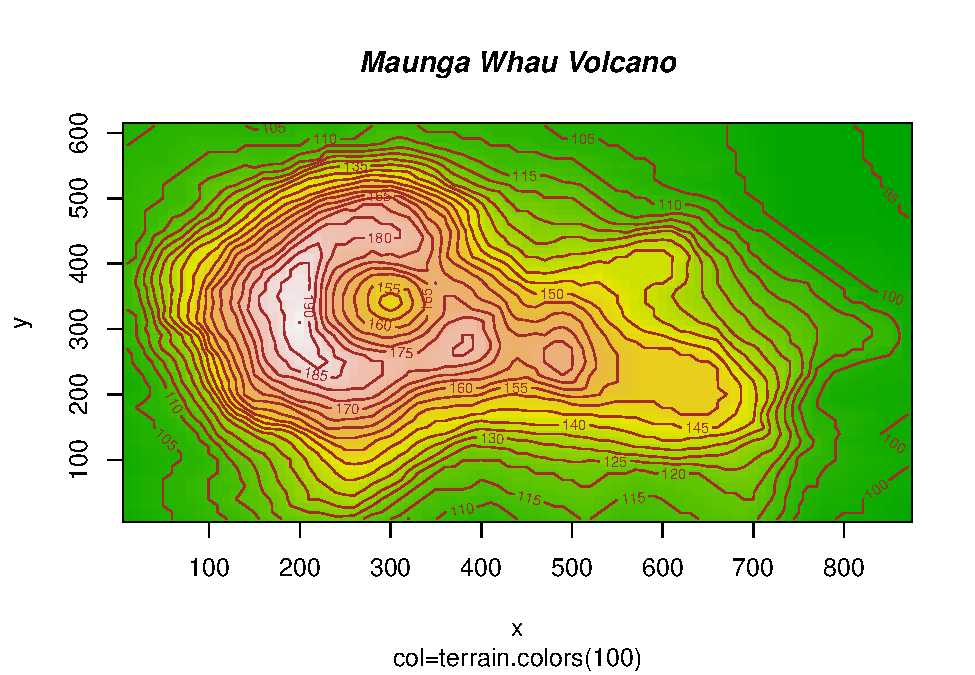
\includegraphics{TudodoR_files/figure-latex/unnamed-chunk-145-1.pdf}

\begin{verbatim}
## 
## > contour(x, y, volcano, levels=seq(90, 200, by=5), add=TRUE, col="brown")
## 
## > axis(1, at=x.at)
## 
## > axis(2, at=y.at)
## 
## > box()
## 
## > title(main="Maunga Whau Volcano", sub = "col=terrain.colors(100)", font.main=4)
## 
## >                    # Using Heat Colors
## > 
## > image(x, y, volcano, col=heat.colors(100), axes=FALSE)
\end{verbatim}

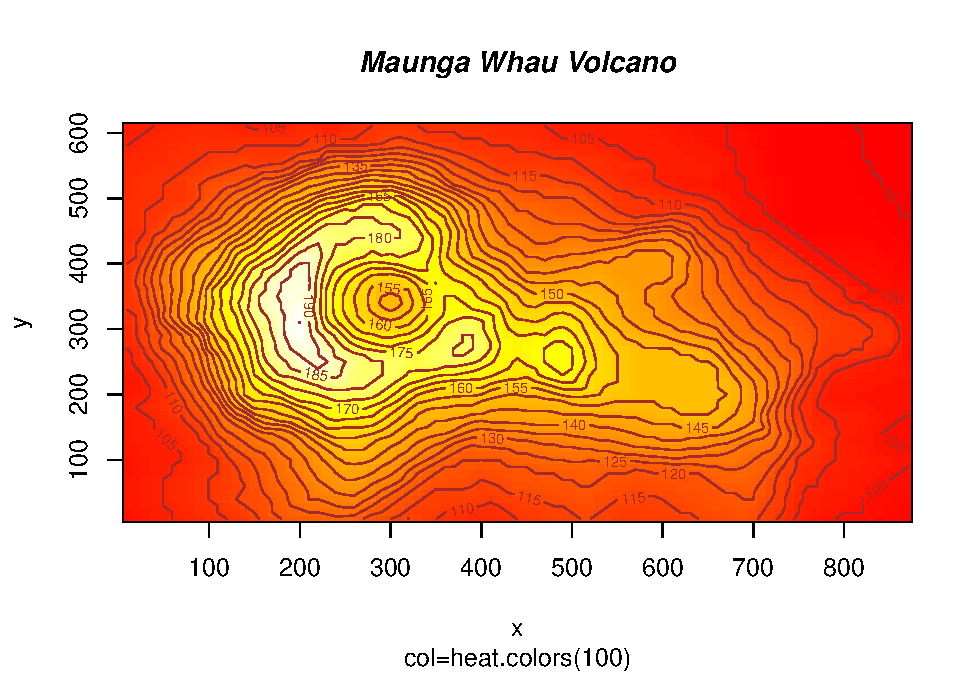
\includegraphics{TudodoR_files/figure-latex/unnamed-chunk-145-2.pdf}

\begin{verbatim}
## 
## > contour(x, y, volcano, levels=seq(90, 200, by=5), add=TRUE, col="brown")
## 
## > axis(1, at=x.at)
## 
## > axis(2, at=y.at)
## 
## > box()
## 
## > title(main="Maunga Whau Volcano", sub = "col=heat.colors(100)", font.main=4)
## 
## >                    # Using Gray Scale
## > 
## > image(x, y, volcano, col=gray(100:200/200), axes=FALSE)
\end{verbatim}

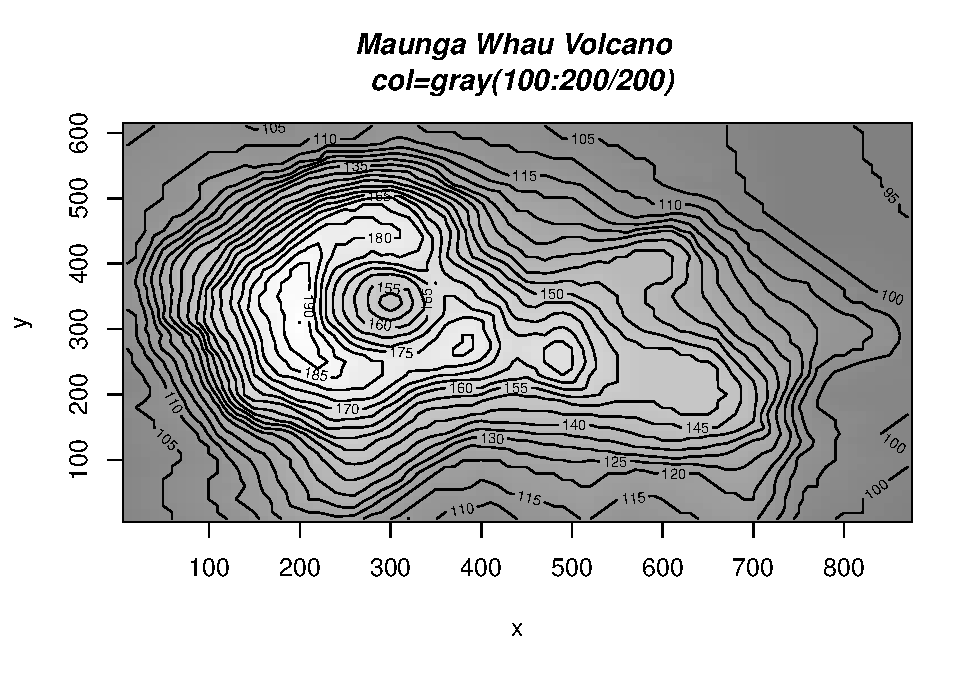
\includegraphics{TudodoR_files/figure-latex/unnamed-chunk-145-3.pdf}

\begin{verbatim}
## 
## > contour(x, y, volcano, levels=seq(90, 200, by=5), add=TRUE, col="black")
## 
## > axis(1, at=x.at)
## 
## > axis(2, at=y.at)
## 
## > box()
## 
## > title(main="Maunga Whau Volcano \n col=gray(100:200/200)", font.main=4)
## 
## > ## Filled Contours are even nicer sometimes :
## > example(filled.contour)
## 
## flld.c> require("grDevices") # for colours
## 
## flld.c> filled.contour(volcano, asp = 1) # simple
\end{verbatim}

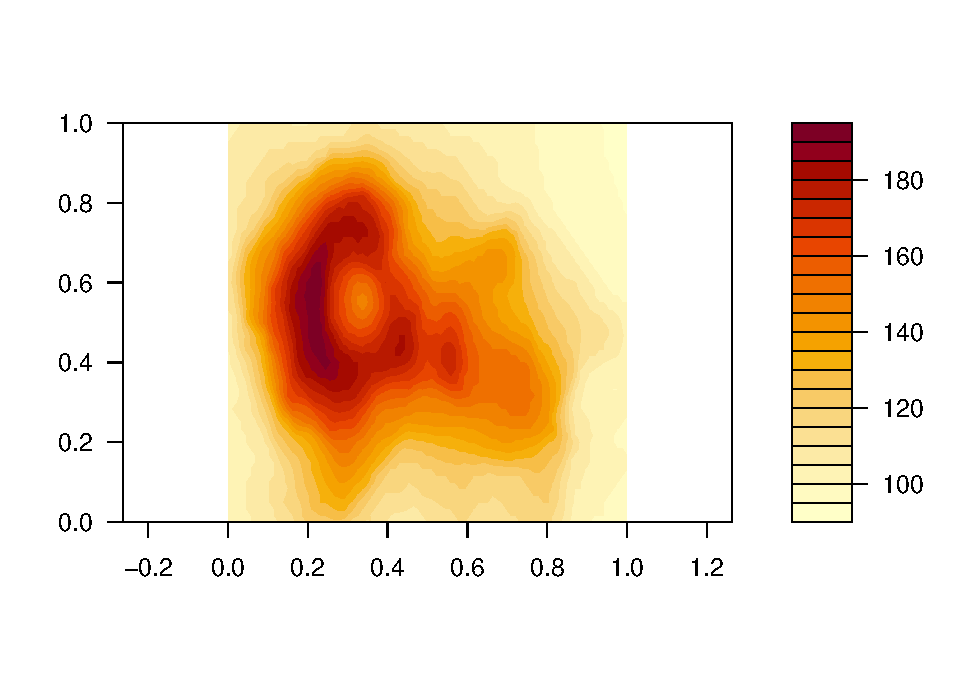
\includegraphics{TudodoR_files/figure-latex/unnamed-chunk-145-4.pdf}

\begin{verbatim}
## 
## flld.c> x <- 10*1:nrow(volcano)
## 
## flld.c> y <- 10*1:ncol(volcano)
## 
## flld.c> filled.contour(x, y, volcano, color = function(n) hcl.colors(n, "terrain"),
## flld.c+     plot.title = title(main = "The Topography of Maunga Whau",
## flld.c+     xlab = "Meters North", ylab = "Meters West"),
## flld.c+     plot.axes = { axis(1, seq(100, 800, by = 100))
## flld.c+                   axis(2, seq(100, 600, by = 100)) },
## flld.c+     key.title = title(main = "Height\n(meters)"),
## flld.c+     key.axes = axis(4, seq(90, 190, by = 10)))  # maybe also asp = 1
\end{verbatim}

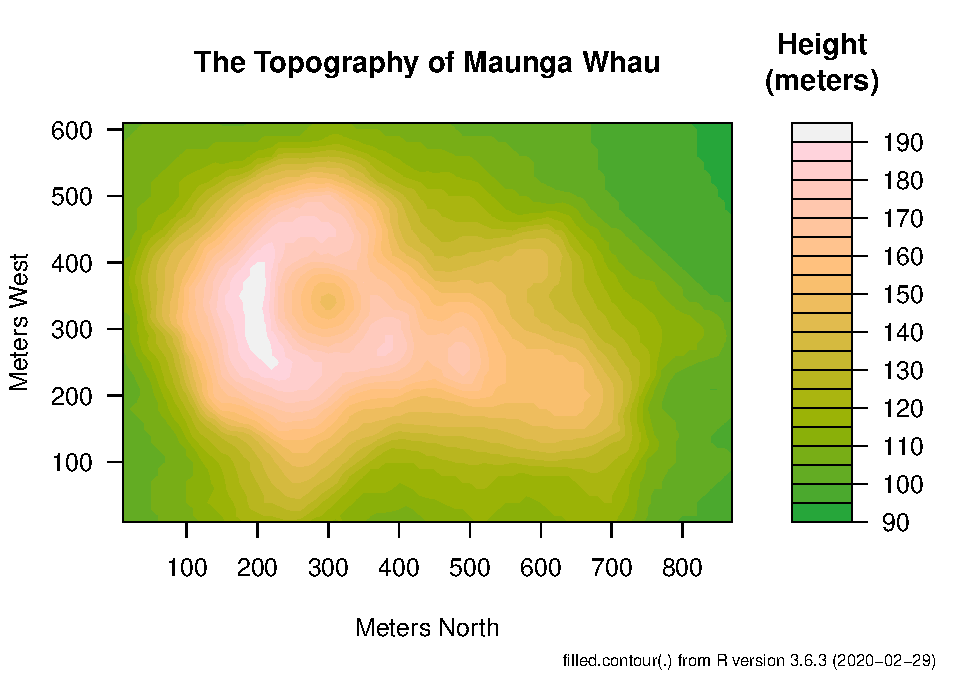
\includegraphics{TudodoR_files/figure-latex/unnamed-chunk-145-5.pdf}

\begin{verbatim}
## 
## flld.c> mtext(paste("filled.contour(.) from", R.version.string),
## flld.c+       side = 1, line = 4, adj = 1, cex = .66)
## 
## flld.c> # Annotating a filled contour plot
## flld.c> a <- expand.grid(1:20, 1:20)
## 
## flld.c> b <- matrix(a[,1] + a[,2], 20)
## 
## flld.c> filled.contour(x = 1:20, y = 1:20, z = b,
## flld.c+                plot.axes = { axis(1); axis(2); points(10, 10) })
\end{verbatim}

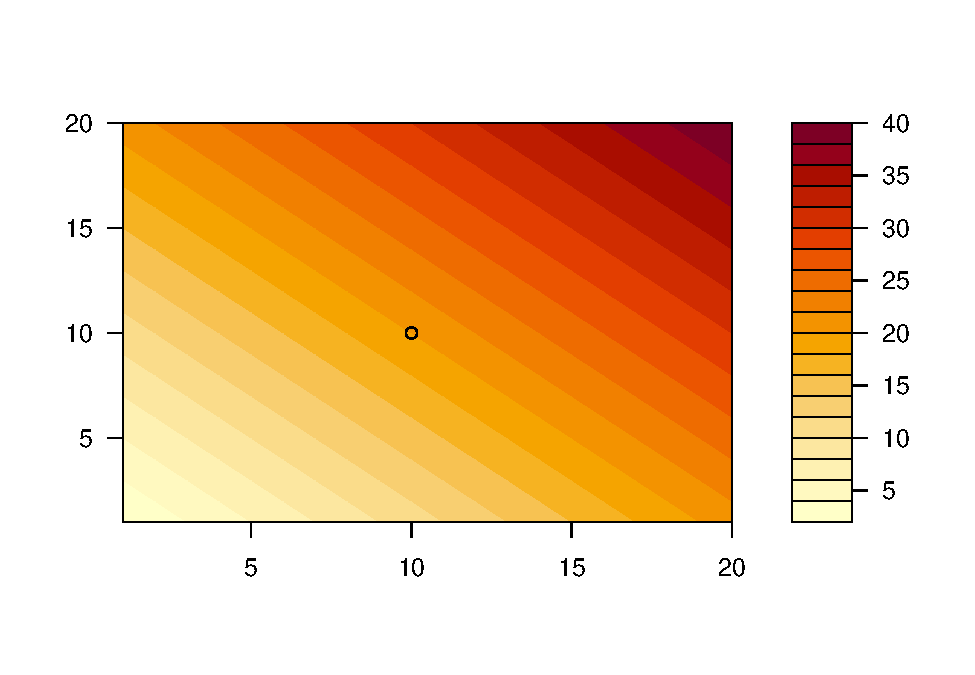
\includegraphics{TudodoR_files/figure-latex/unnamed-chunk-145-6.pdf}

\begin{verbatim}
## 
## flld.c> ## Persian Rug Art:
## flld.c> x <- y <- seq(-4*pi, 4*pi, len = 27)
## 
## flld.c> r <- sqrt(outer(x^2, y^2, "+"))
## 
## flld.c> filled.contour(cos(r^2)*exp(-r/(2*pi)), axes = FALSE)
\end{verbatim}

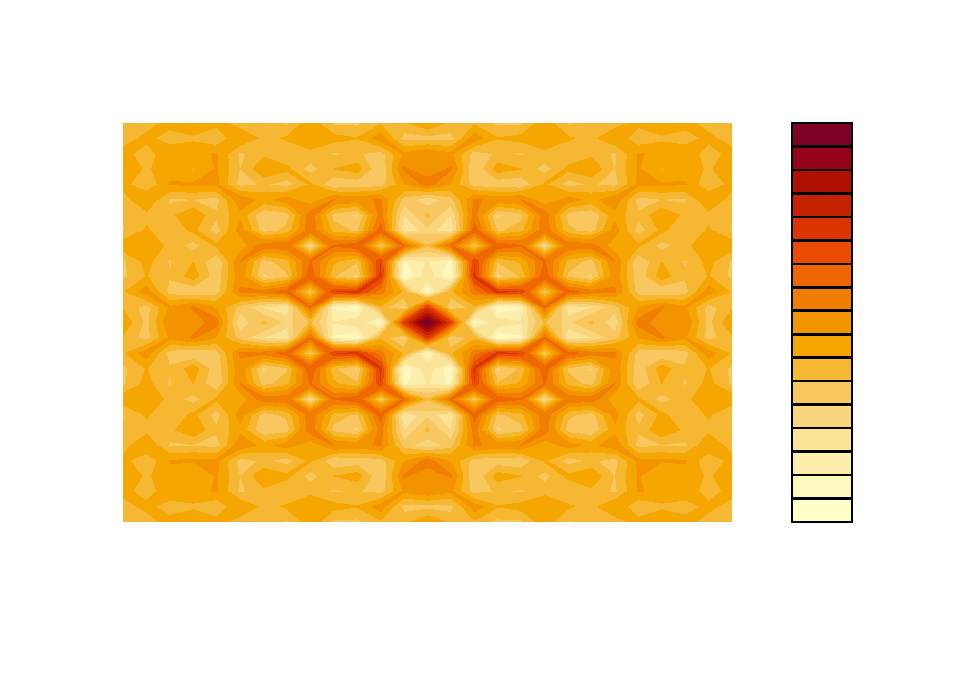
\includegraphics{TudodoR_files/figure-latex/unnamed-chunk-145-7.pdf}

\begin{verbatim}
## 
## flld.c> ## rather, the key *should* be labeled:
## flld.c> filled.contour(cos(r^2)*exp(-r/(2*pi)), frame.plot = FALSE,
## flld.c+                plot.axes = {})
\end{verbatim}

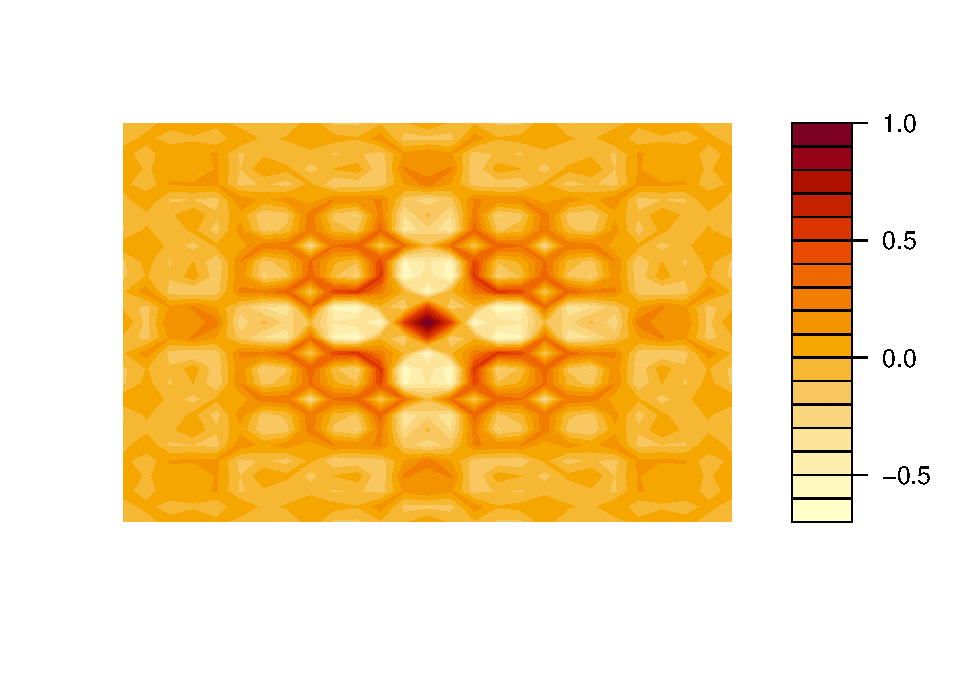
\includegraphics{TudodoR_files/figure-latex/unnamed-chunk-145-8.pdf}

\begin{Shaded}
\begin{Highlighting}[]
\KeywordTok{demo}\NormalTok{(persp)}
\end{Highlighting}
\end{Shaded}

\begin{verbatim}
## 
## 
##  demo(persp)
##  ---- ~~~~~
## 
## > ### Demos for  persp()  plots   -- things not in  example(persp)
## > ### -------------------------
## > 
## > require(datasets)
## 
## > require(grDevices); require(graphics)
## 
## > ## (1) The Obligatory Mathematical surface.
## > ##     Rotated sinc function.
## > 
## > x <- seq(-10, 10, length.out = 50)
## 
## > y <- x
## 
## > rotsinc <- function(x,y)
## + {
## +     sinc <- function(x) { y <- sin(x)/x ; y[is.na(y)] <- 1; y }
## +     10 * sinc( sqrt(x^2+y^2) )
## + }
## 
## > sinc.exp <- expression(z == Sinc(sqrt(x^2 + y^2)))
## 
## > z <- outer(x, y, rotsinc)
## 
## > oldpar <- par(bg = "white")
## 
## > persp(x, y, z, theta = 30, phi = 30, expand = 0.5, col = "lightblue")
\end{verbatim}

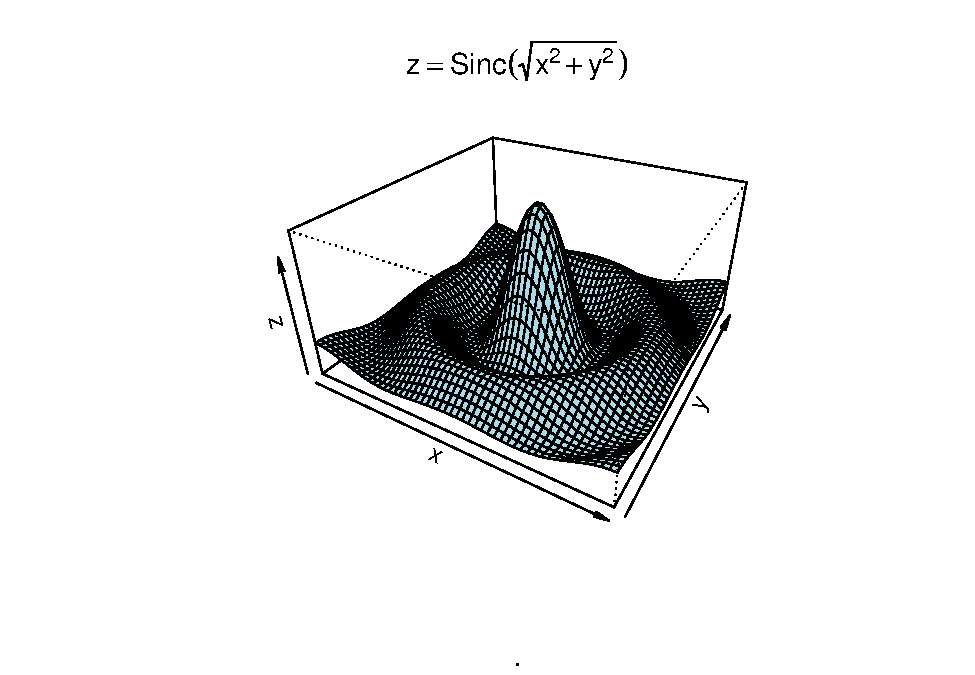
\includegraphics{TudodoR_files/figure-latex/unnamed-chunk-146-1.pdf}

\begin{verbatim}
## 
## > title(sub=".")## work around persp+plotmath bug
## 
## > title(main = sinc.exp)
## 
## > persp(x, y, z, theta = 30, phi = 30, expand = 0.5, col = "lightblue",
## +       ltheta = 120, shade = 0.75, ticktype = "detailed",
## +       xlab = "X", ylab = "Y", zlab = "Z")
\end{verbatim}

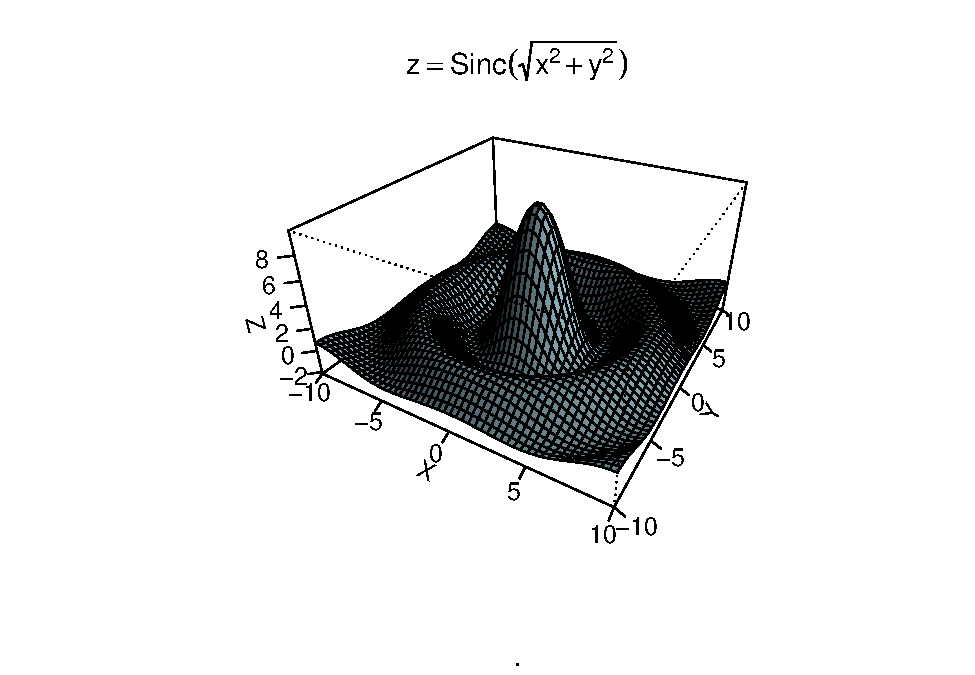
\includegraphics{TudodoR_files/figure-latex/unnamed-chunk-146-2.pdf}

\begin{verbatim}
## 
## > title(sub=".")## work around persp+plotmath bug
## 
## > title(main = sinc.exp)
## 
## > ## (2) Visualizing a simple DEM model
## > 
## > z <- 2 * volcano        # Exaggerate the relief
## 
## > x <- 10 * (1:nrow(z))   # 10 meter spacing (S to N)
## 
## > y <- 10 * (1:ncol(z))   # 10 meter spacing (E to W)
## 
## > persp(x, y, z, theta = 120, phi = 15, scale = FALSE, axes = FALSE)
\end{verbatim}

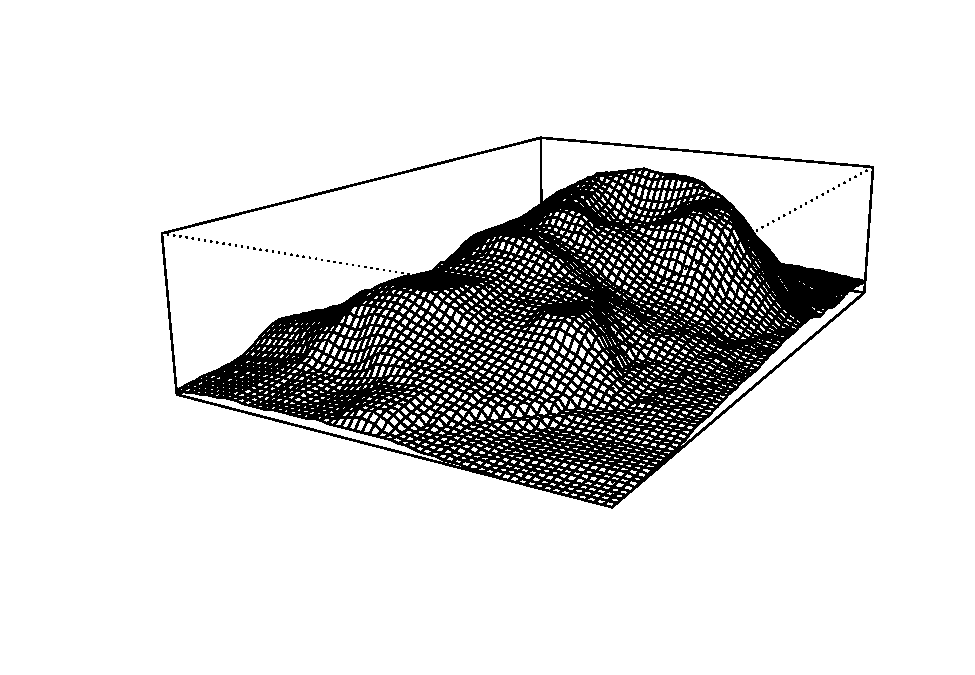
\includegraphics{TudodoR_files/figure-latex/unnamed-chunk-146-3.pdf}

\begin{verbatim}
## 
## > ## (3) Now something more complex
## > ##     We border the surface, to make it more "slice like"
## > ##     and color the top and sides of the surface differently.
## > 
## > z0 <- min(z) - 20
## 
## > z <- rbind(z0, cbind(z0, z, z0), z0)
## 
## > x <- c(min(x) - 1e-10, x, max(x) + 1e-10)
## 
## > y <- c(min(y) - 1e-10, y, max(y) + 1e-10)
## 
## > fill <- matrix("green3", nrow = nrow(z)-1, ncol = ncol(z)-1)
## 
## > fill[ , i2 <- c(1,ncol(fill))] <- "gray"
## 
## > fill[i1 <- c(1,nrow(fill)) , ] <- "gray"
## 
## > par(bg = "lightblue")
## 
## > persp(x, y, z, theta = 120, phi = 15, col = fill, scale = FALSE, axes = FALSE)
\end{verbatim}

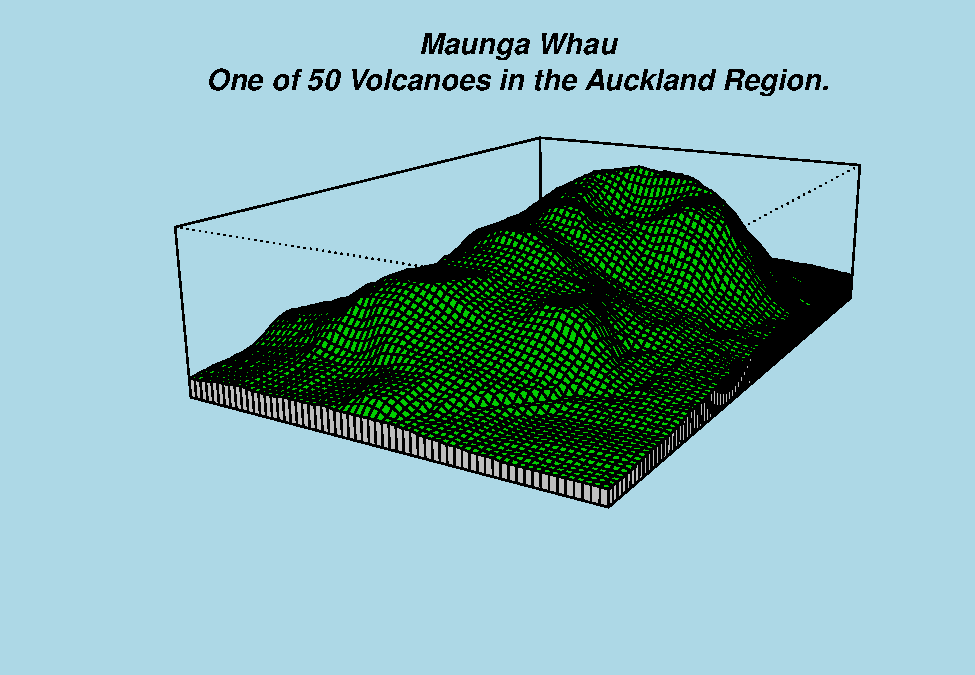
\includegraphics{TudodoR_files/figure-latex/unnamed-chunk-146-4.pdf}

\begin{verbatim}
## 
## > title(main = "Maunga Whau\nOne of 50 Volcanoes in the Auckland Region.",
## +       font.main = 4)
## 
## > par(bg = "slategray")
## 
## > persp(x, y, z, theta = 135, phi = 30, col = fill, scale = FALSE,
## +       ltheta = -120, lphi = 15, shade = 0.65, axes = FALSE)
\end{verbatim}

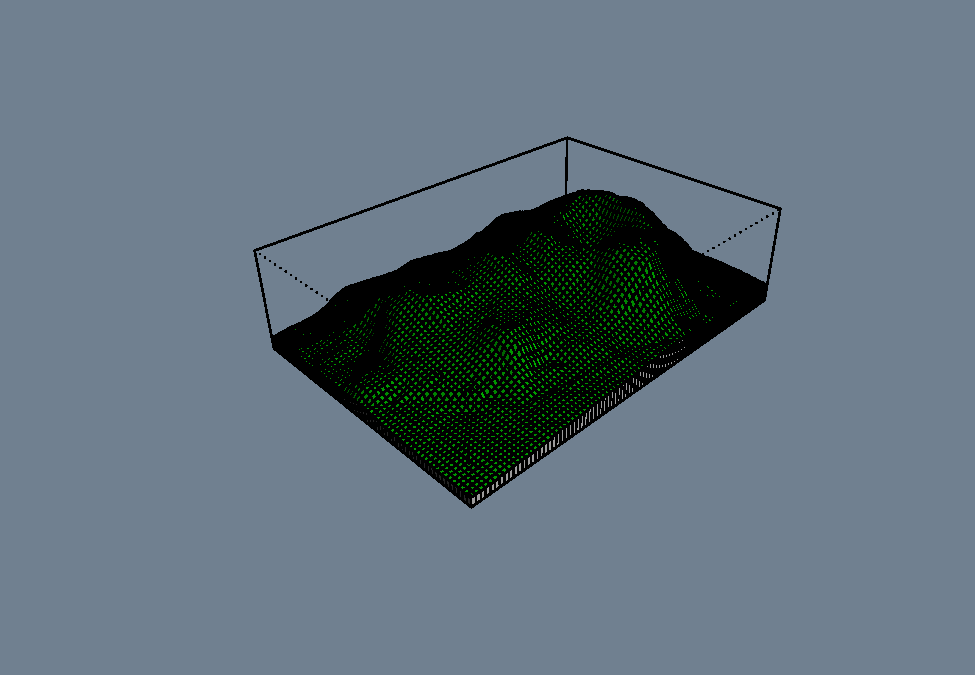
\includegraphics{TudodoR_files/figure-latex/unnamed-chunk-146-5.pdf}

\begin{verbatim}
## 
## > ## Don't draw the grid lines :  border = NA
## > persp(x, y, z, theta = 135, phi = 30, col = "green3", scale = FALSE,
## +       ltheta = -120, shade = 0.75, border = NA, box = FALSE)
\end{verbatim}

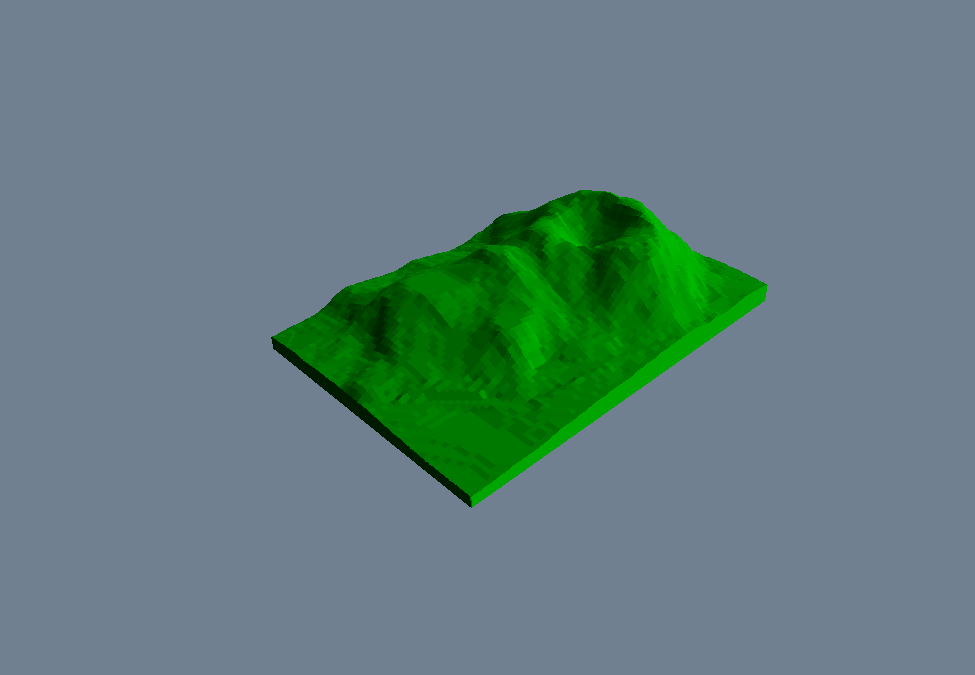
\includegraphics{TudodoR_files/figure-latex/unnamed-chunk-146-6.pdf}

\begin{verbatim}
## 
## > ## `color gradient in the soil' :
## > fcol <- fill ; fcol[] <- terrain.colors(nrow(fcol))
## 
## > persp(x, y, z, theta = 135, phi = 30, col = fcol, scale = FALSE,
## +       ltheta = -120, shade = 0.3, border = NA, box = FALSE)
\end{verbatim}

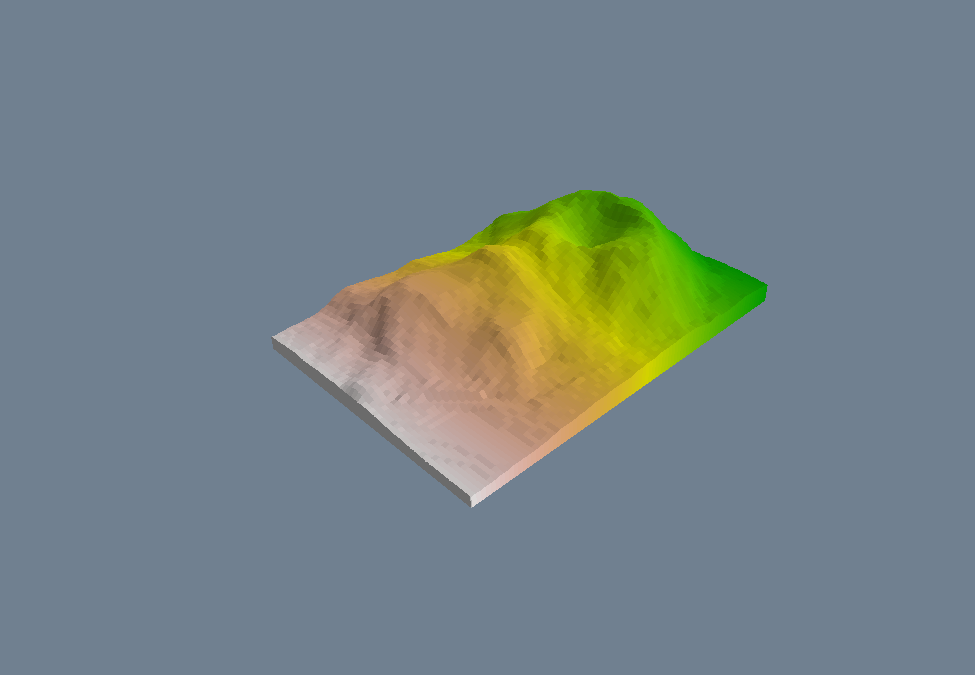
\includegraphics{TudodoR_files/figure-latex/unnamed-chunk-146-7.pdf}

\begin{verbatim}
## 
## > ## `image like' colors on top :
## > fcol <- fill
## 
## > zi <- volcano[ -1,-1] + volcano[ -1,-61] +
## +            volcano[-87,-1] + volcano[-87,-61]  ## / 4
## 
## > fcol[-i1,-i2] <-
## +     terrain.colors(20)[cut(zi,
## +                            stats::quantile(zi, seq(0,1, length.out = 21)),
## +                            include.lowest = TRUE)]
## 
## > persp(x, y, 2*z, theta = 110, phi = 40, col = fcol, scale = FALSE,
## +       ltheta = -120, shade = 0.4, border = NA, box = FALSE)
\end{verbatim}

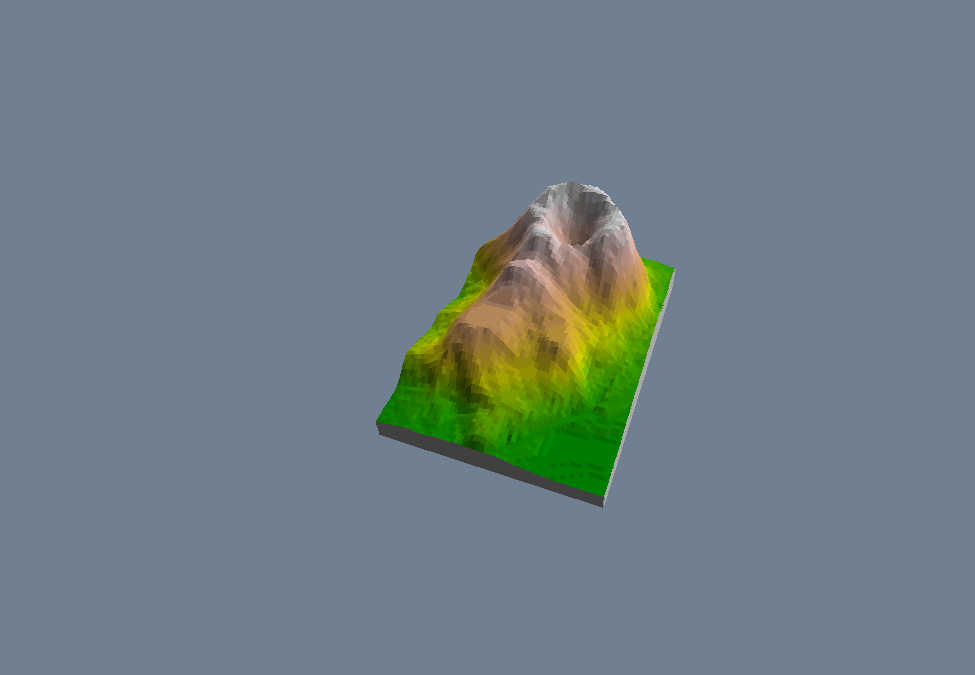
\includegraphics{TudodoR_files/figure-latex/unnamed-chunk-146-8.pdf}

\begin{verbatim}
## 
## > ## reset par():
## > par(oldpar)
\end{verbatim}

\begin{Shaded}
\begin{Highlighting}[]
\KeywordTok{demo}\NormalTok{(graphics)}
\end{Highlighting}
\end{Shaded}

\begin{verbatim}
## 
## 
##  demo(graphics)
##  ---- ~~~~~~~~
## 
## > #  Copyright (C) 1997-2009 The R Core Team
## > 
## > require(datasets)
## 
## > require(grDevices); require(graphics)
## 
## > ## Here is some code which illustrates some of the differences between
## > ## R and S graphics capabilities.  Note that colors are generally specified
## > ## by a character string name (taken from the X11 rgb.txt file) and that line
## > ## textures are given similarly.  The parameter "bg" sets the background
## > ## parameter for the plot and there is also an "fg" parameter which sets
## > ## the foreground color.
## > 
## > 
## > x <- stats::rnorm(50)
## 
## > opar <- par(bg = "white")
## 
## > plot(x, ann = FALSE, type = "n")
\end{verbatim}

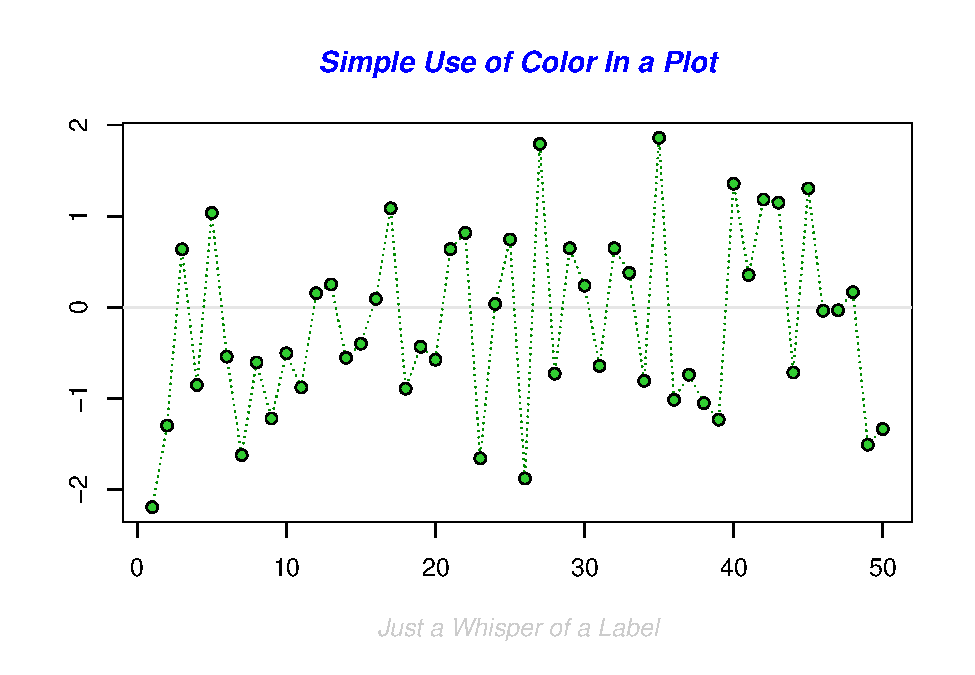
\includegraphics{TudodoR_files/figure-latex/unnamed-chunk-147-1.pdf}

\begin{verbatim}
## 
## > abline(h = 0, col = gray(.90))
## 
## > lines(x, col = "green4", lty = "dotted")
## 
## > points(x, bg = "limegreen", pch = 21)
## 
## > title(main = "Simple Use of Color In a Plot",
## +       xlab = "Just a Whisper of a Label",
## +       col.main = "blue", col.lab = gray(.8),
## +       cex.main = 1.2, cex.lab = 1.0, font.main = 4, font.lab = 3)
## 
## > ## A little color wheel.    This code just plots equally spaced hues in
## > ## a pie chart.    If you have a cheap SVGA monitor (like me) you will
## > ## probably find that numerically equispaced does not mean visually
## > ## equispaced.  On my display at home, these colors tend to cluster at
## > ## the RGB primaries.  On the other hand on the SGI Indy at work the
## > ## effect is near perfect.
## > 
## > par(bg = "gray")
## 
## > pie(rep(1,24), col = rainbow(24), radius = 0.9)
\end{verbatim}

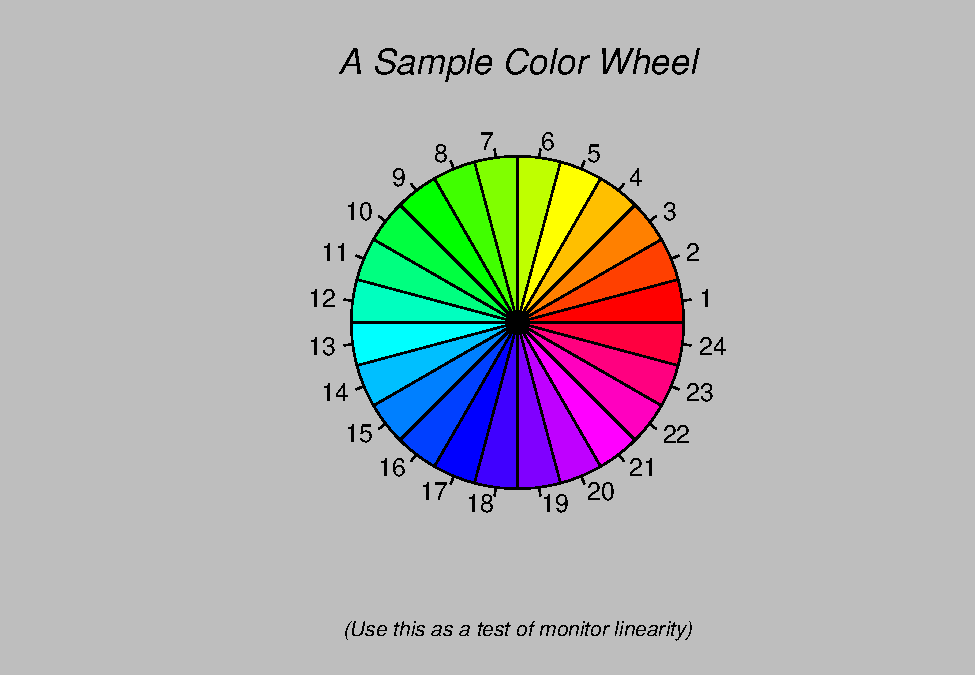
\includegraphics{TudodoR_files/figure-latex/unnamed-chunk-147-2.pdf}

\begin{verbatim}
## 
## > title(main = "A Sample Color Wheel", cex.main = 1.4, font.main = 3)
## 
## > title(xlab = "(Use this as a test of monitor linearity)",
## +       cex.lab = 0.8, font.lab = 3)
## 
## > ## We have already confessed to having these.  This is just showing off X11
## > ## color names (and the example (from the postscript manual) is pretty "cute".
## > 
## > pie.sales <- c(0.12, 0.3, 0.26, 0.16, 0.04, 0.12)
## 
## > names(pie.sales) <- c("Blueberry", "Cherry",
## +              "Apple", "Boston Cream", "Other", "Vanilla Cream")
## 
## > pie(pie.sales,
## +     col = c("purple","violetred1","green3","cornsilk","cyan","white"))
\end{verbatim}

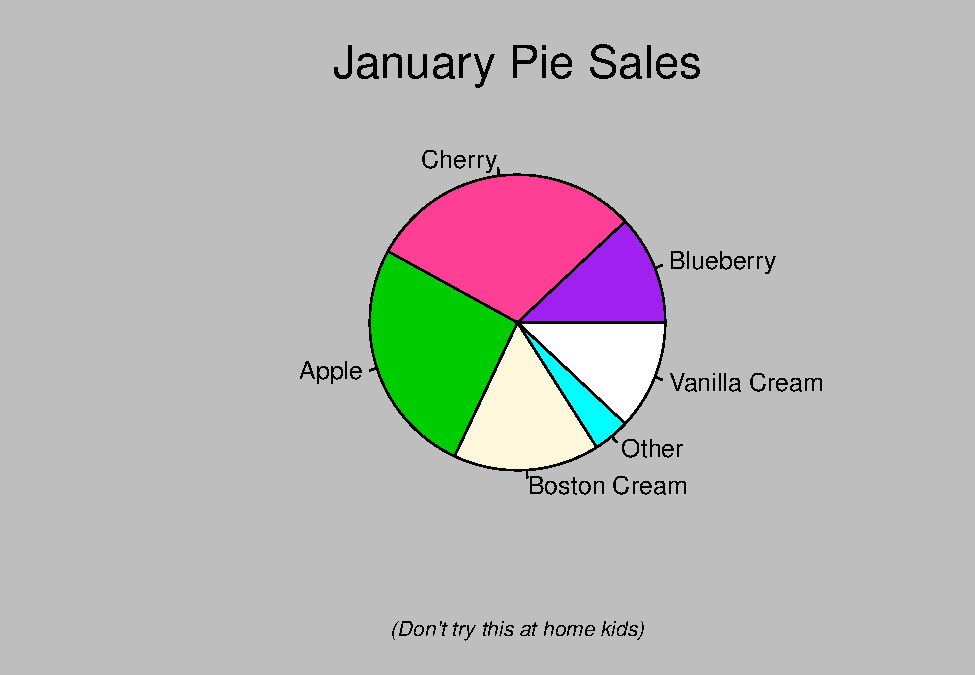
\includegraphics{TudodoR_files/figure-latex/unnamed-chunk-147-3.pdf}

\begin{verbatim}
## 
## > title(main = "January Pie Sales", cex.main = 1.8, font.main = 1)
## 
## > title(xlab = "(Don't try this at home kids)", cex.lab = 0.8, font.lab = 3)
## 
## > ## Boxplots:  I couldn't resist the capability for filling the "box".
## > ## The use of color seems like a useful addition, it focuses attention
## > ## on the central bulk of the data.
## > 
## > par(bg="cornsilk")
## 
## > n <- 10
## 
## > g <- gl(n, 100, n*100)
## 
## > x <- rnorm(n*100) + sqrt(as.numeric(g))
## 
## > boxplot(split(x,g), col="lavender", notch=TRUE)
\end{verbatim}

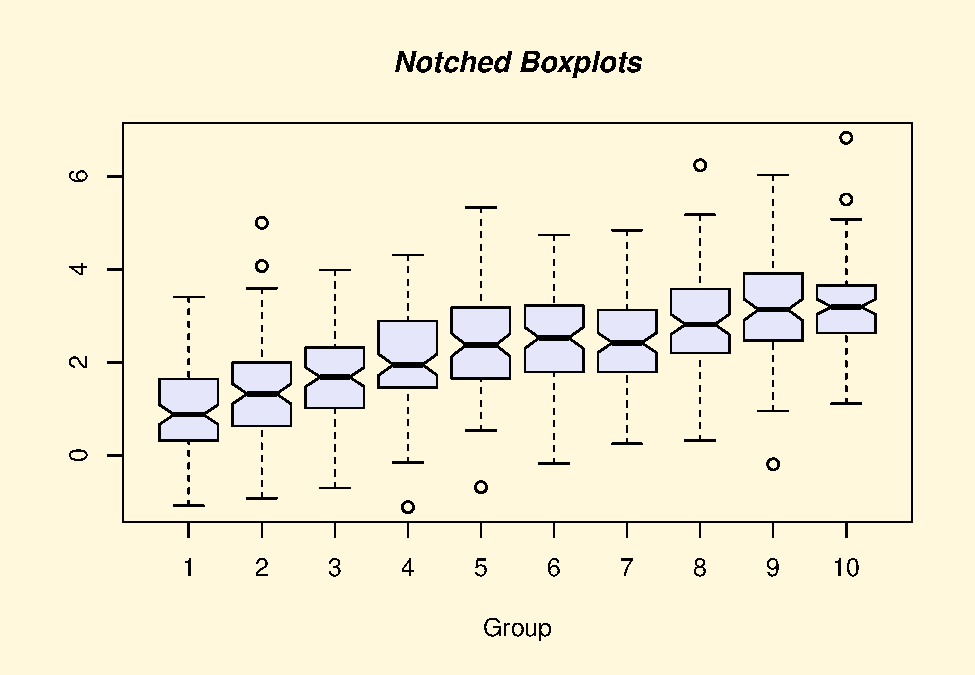
\includegraphics{TudodoR_files/figure-latex/unnamed-chunk-147-4.pdf}

\begin{verbatim}
## 
## > title(main="Notched Boxplots", xlab="Group", font.main=4, font.lab=1)
## 
## > ## An example showing how to fill between curves.
## > 
## > par(bg="white")
## 
## > n <- 100
## 
## > x <- c(0,cumsum(rnorm(n)))
## 
## > y <- c(0,cumsum(rnorm(n)))
## 
## > xx <- c(0:n, n:0)
## 
## > yy <- c(x, rev(y))
## 
## > plot(xx, yy, type="n", xlab="Time", ylab="Distance")
\end{verbatim}

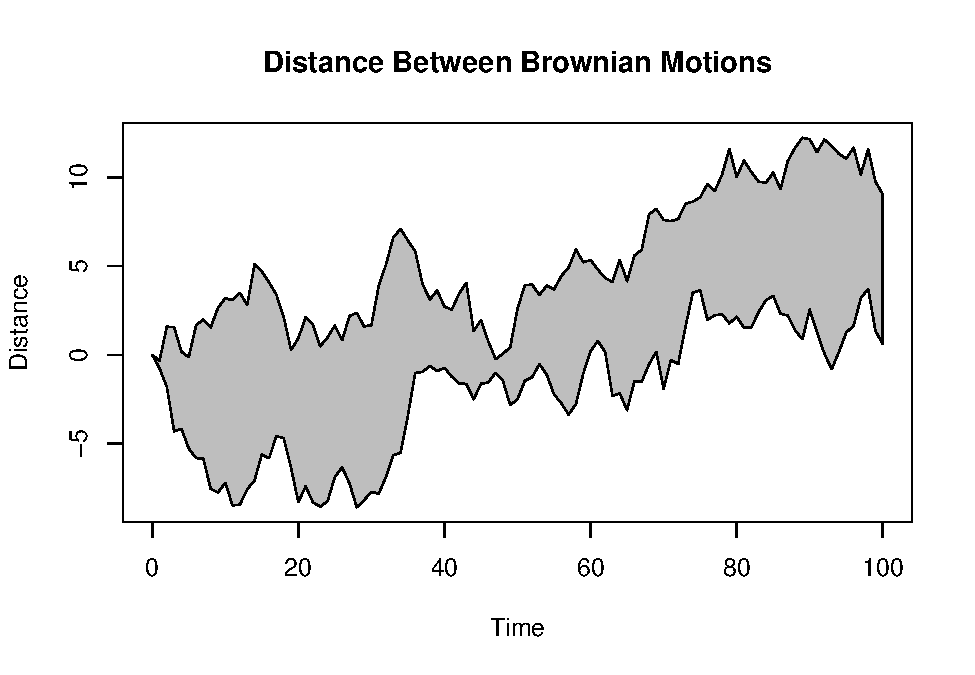
\includegraphics{TudodoR_files/figure-latex/unnamed-chunk-147-5.pdf}

\begin{verbatim}
## 
## > polygon(xx, yy, col="gray")
## 
## > title("Distance Between Brownian Motions")
## 
## > ## Colored plot margins, axis labels and titles.    You do need to be
## > ## careful with these kinds of effects.    It's easy to go completely
## > ## over the top and you can end up with your lunch all over the keyboard.
## > ## On the other hand, my market research clients love it.
## > 
## > x <- c(0.00, 0.40, 0.86, 0.85, 0.69, 0.48, 0.54, 1.09, 1.11, 1.73, 2.05, 2.02)
## 
## > par(bg="lightgray")
## 
## > plot(x, type="n", axes=FALSE, ann=FALSE)
\end{verbatim}

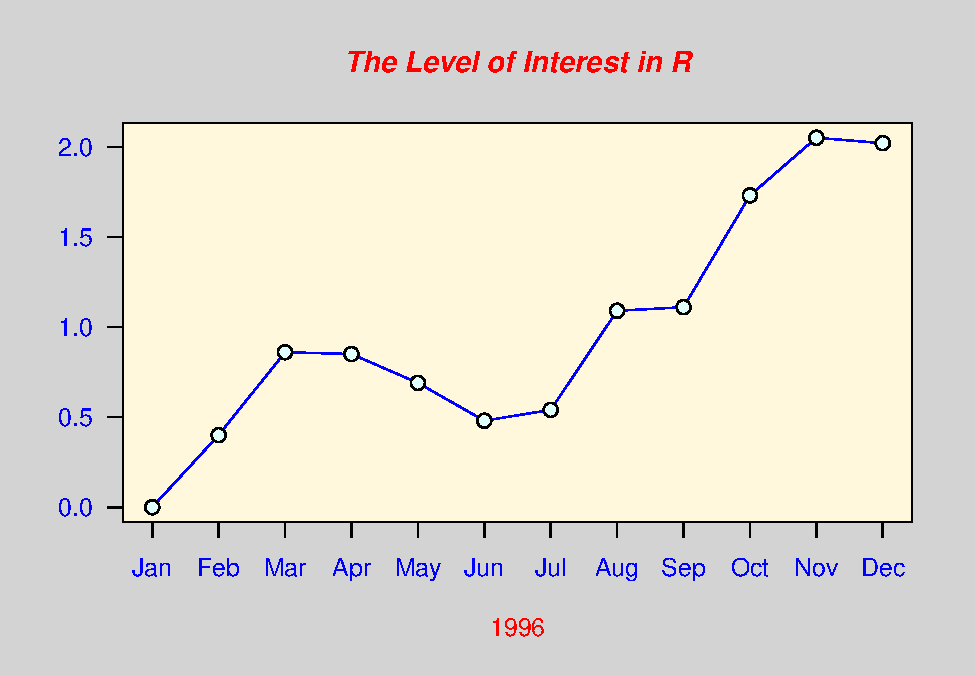
\includegraphics{TudodoR_files/figure-latex/unnamed-chunk-147-6.pdf}

\begin{verbatim}
## 
## > usr <- par("usr")
## 
## > rect(usr[1], usr[3], usr[2], usr[4], col="cornsilk", border="black")
## 
## > lines(x, col="blue")
## 
## > points(x, pch=21, bg="lightcyan", cex=1.25)
## 
## > axis(2, col.axis="blue", las=1)
## 
## > axis(1, at=1:12, lab=month.abb, col.axis="blue")
## 
## > box()
## 
## > title(main= "The Level of Interest in R", font.main=4, col.main="red")
## 
## > title(xlab= "1996", col.lab="red")
## 
## > ## A filled histogram, showing how to change the font used for the
## > ## main title without changing the other annotation.
## > 
## > par(bg="cornsilk")
## 
## > x <- rnorm(1000)
## 
## > hist(x, xlim=range(-4, 4, x), col="lavender", main="")
\end{verbatim}

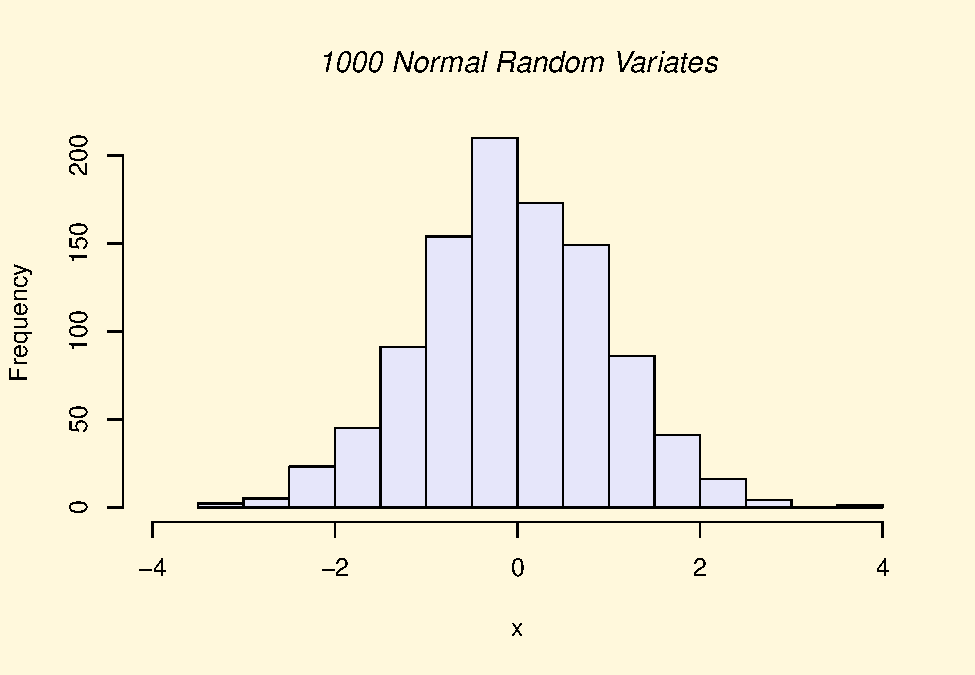
\includegraphics{TudodoR_files/figure-latex/unnamed-chunk-147-7.pdf}

\begin{verbatim}
## 
## > title(main="1000 Normal Random Variates", font.main=3)
## 
## > ## A scatterplot matrix
## > ## The good old Iris data (yet again)
## > 
## > pairs(iris[1:4], main="Edgar Anderson's Iris Data", font.main=4, pch=19)
\end{verbatim}

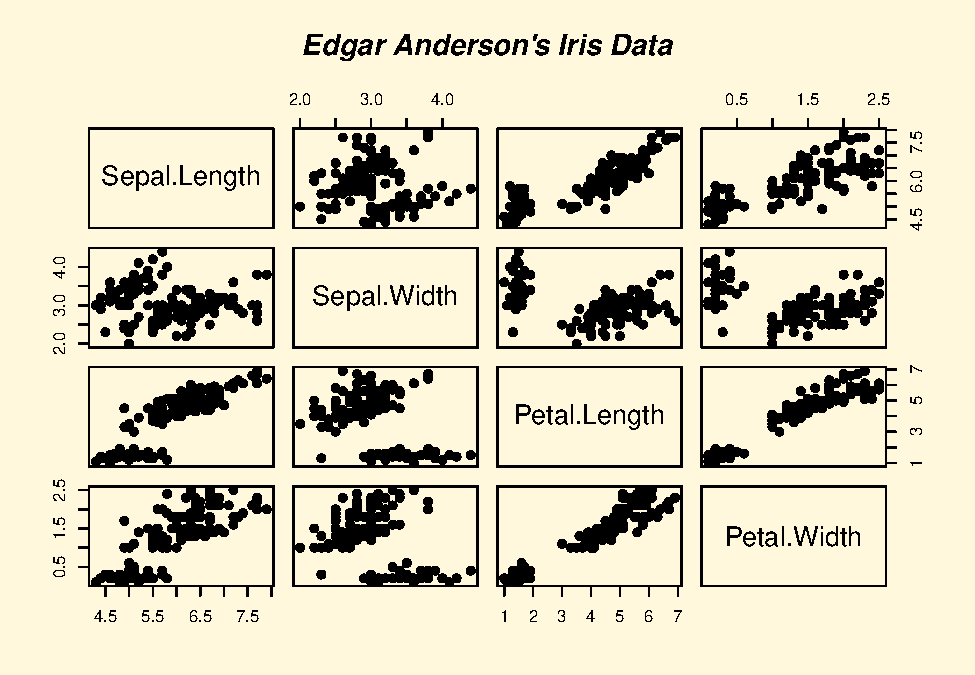
\includegraphics{TudodoR_files/figure-latex/unnamed-chunk-147-8.pdf}

\begin{verbatim}
## 
## > pairs(iris[1:4], main="Edgar Anderson's Iris Data", pch=21,
## +       bg = c("red", "green3", "blue")[unclass(iris$Species)])
\end{verbatim}

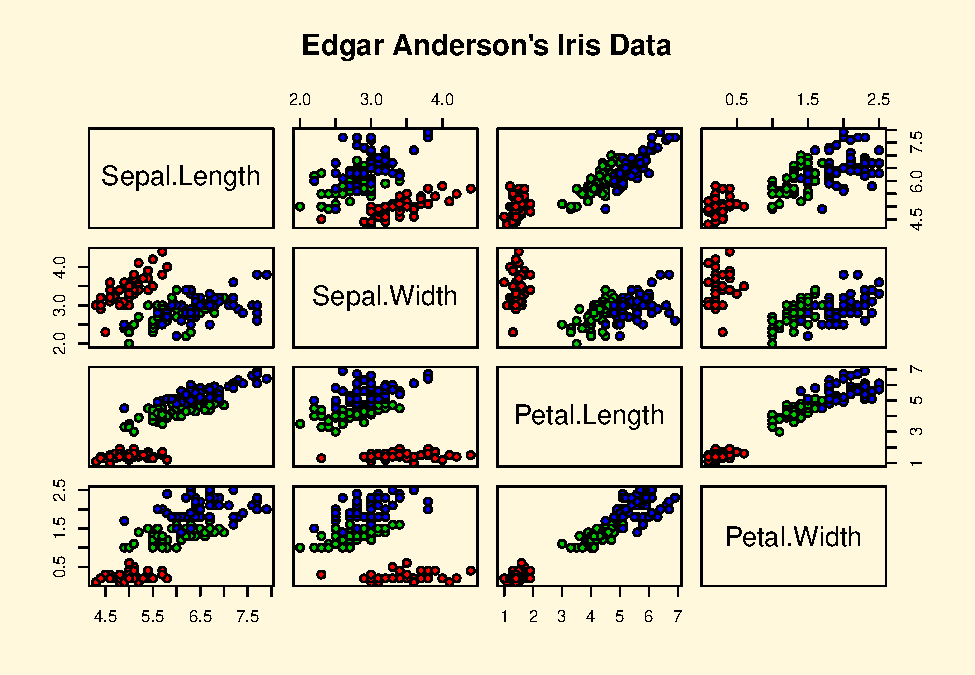
\includegraphics{TudodoR_files/figure-latex/unnamed-chunk-147-9.pdf}

\begin{verbatim}
## 
## > ## Contour plotting
## > ## This produces a topographic map of one of Auckland's many volcanic "peaks".
## > 
## > x <- 10*1:nrow(volcano)
## 
## > y <- 10*1:ncol(volcano)
## 
## > lev <- pretty(range(volcano), 10)
## 
## > par(bg = "lightcyan")
## 
## > pin <- par("pin")
## 
## > xdelta <- diff(range(x))
## 
## > ydelta <- diff(range(y))
## 
## > xscale <- pin[1]/xdelta
## 
## > yscale <- pin[2]/ydelta
## 
## > scale <- min(xscale, yscale)
## 
## > xadd <- 0.5*(pin[1]/scale - xdelta)
## 
## > yadd <- 0.5*(pin[2]/scale - ydelta)
## 
## > plot(numeric(0), numeric(0),
## +      xlim = range(x)+c(-1,1)*xadd, ylim = range(y)+c(-1,1)*yadd,
## +      type = "n", ann = FALSE)
\end{verbatim}

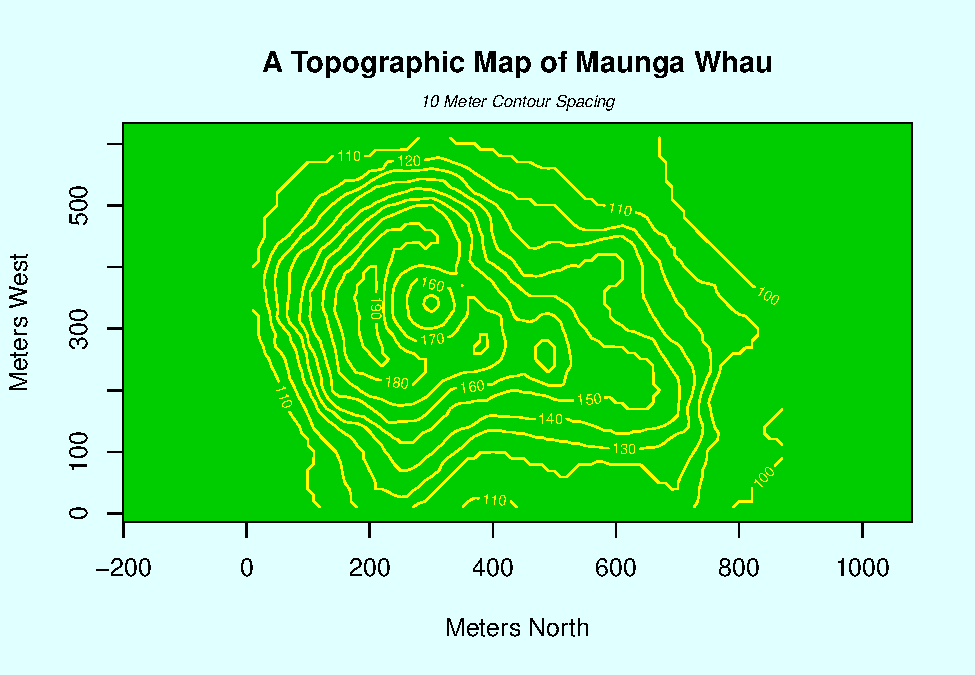
\includegraphics{TudodoR_files/figure-latex/unnamed-chunk-147-10.pdf}

\begin{verbatim}
## 
## > usr <- par("usr")
## 
## > rect(usr[1], usr[3], usr[2], usr[4], col="green3")
## 
## > contour(x, y, volcano, levels = lev, col="yellow", lty="solid", add=TRUE)
## 
## > box()
## 
## > title("A Topographic Map of Maunga Whau", font= 4)
## 
## > title(xlab = "Meters North", ylab = "Meters West", font= 3)
## 
## > mtext("10 Meter Contour Spacing", side=3, line=0.35, outer=FALSE,
## +       at = mean(par("usr")[1:2]), cex=0.7, font=3)
## 
## > ## Conditioning plots
## > 
## > par(bg="cornsilk")
## 
## > coplot(lat ~ long | depth, data = quakes, pch = 21, bg = "green3")
\end{verbatim}

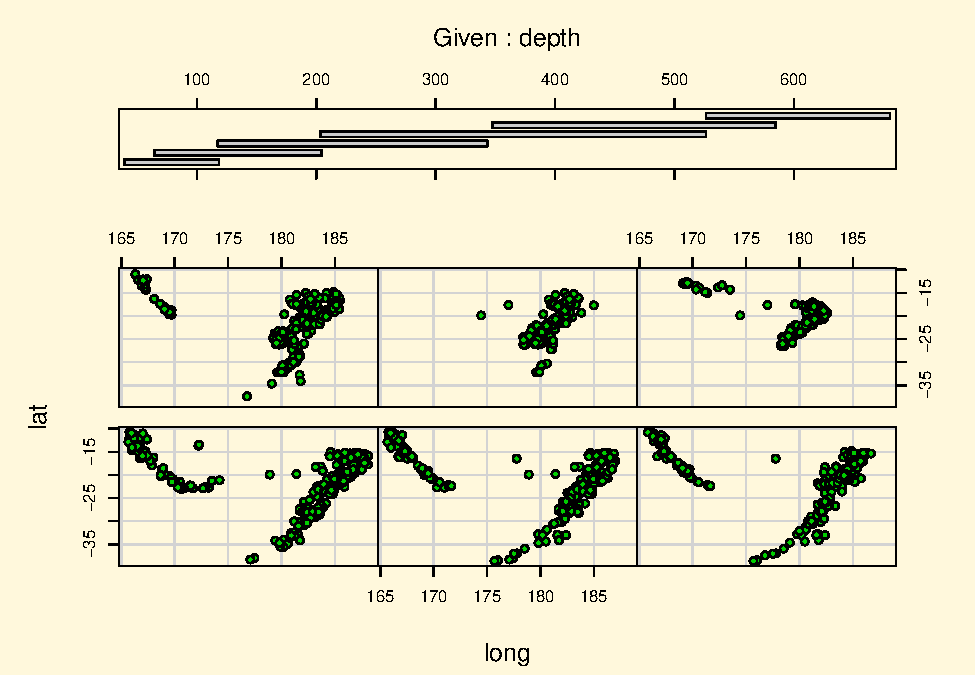
\includegraphics{TudodoR_files/figure-latex/unnamed-chunk-147-11.pdf}

\begin{verbatim}
## 
## > par(opar)
\end{verbatim}

\hypertarget{entrada-de-dados-1}{%
\section{Entrada de dados}\label{entrada-de-dados-1}}

Nesse tópico utlizaremos o arquivo de dados \href{https://www.dropbox.com/s/zg7fyg1iewtji49/dadosfisio.csv?dl=1}{dadosfisio.csv}.

Dados fisico hidrico de 3 solos com textutas diferentes.

\begin{longtable}[]{@{}lllll@{}}
\toprule
Cod. & Solo & Areia & Silte & Argila\tabularnewline
\midrule
\endhead
Z1 & NITOSSOLO & 122 & 121 & 757\tabularnewline
Z2 & LATOSSOLO & 710 & 80 & 210\tabularnewline
Z3 & LATOSSOLO & 892 & 10 & 98\tabularnewline
\bottomrule
\end{longtable}

Ler dados via web.

\begin{Shaded}
\begin{Highlighting}[]
\NormalTok{solo <-}\StringTok{ }\KeywordTok{read.table}\NormalTok{(}\StringTok{"https://www.dropbox.com/s/zg7fyg1iewtji49/dadosfisio.csv?dl=1"}\NormalTok{, }\DataTypeTok{sep =} \StringTok{";"}\NormalTok{, }\DataTypeTok{header =}\NormalTok{ T, }\DataTypeTok{dec =} \StringTok{","}\NormalTok{)}
\end{Highlighting}
\end{Shaded}

Verificar a estrutura de dados.

\begin{Shaded}
\begin{Highlighting}[]
\KeywordTok{str}\NormalTok{(solo)}
\end{Highlighting}
\end{Shaded}

\begin{verbatim}
## 'data.frame':    108 obs. of  16 variables:
##  $ z     : int  1 1 1 1 1 1 1 1 1 1 ...
##  $ x     : int  1 1 1 1 1 1 3 3 3 3 ...
##  $ y     : int  1 3 5 7 9 11 1 3 5 7 ...
##  $ cota  : num  9.15 8.95 8.78 8.59 8.48 8.41 8.93 8.76 8.58 8.48 ...
##  $ ds    : num  1.5 1.47 1.47 1.39 1.38 ...
##  $ cc    : num  0.398 0.382 0.351 0.372 0.356 ...
##  $ ma    : num  0.129 0.153 0.185 0.188 0.208 ...
##  $ ptotal: num  0.526 0.535 0.537 0.561 0.564 ...
##  $ tibo  : num  46.1 19.2 172.8 96 30.7 ...
##  $ tibe  : num  26.8 26.1 113.9 74.8 37.2 ...
##  $ a     : num  926 384 275 1207 151 ...
##  $ b     : num  -0.529 -0.418 -0.131 -0.376 -0.227 ...
##  $ X3    : num  518 243 238 798 118 ...
##  $ X60   : num  153.2 92.7 176.5 335.4 69.9 ...
##  $ X90   : num  106.2 69.4 161.2 258.4 59.8 ...
##  $ X120  : num  73.6 52 147.2 199 51.1 ...
\end{verbatim}

Resumo estatástico da coluna 5 a coluna 8 de todos os solos

\begin{Shaded}
\begin{Highlighting}[]
\KeywordTok{summary}\NormalTok{(solo[}\DecValTok{5}\OperatorTok{:}\DecValTok{8}\NormalTok{])}
\end{Highlighting}
\end{Shaded}

\begin{verbatim}
##        ds              cc               ma               ptotal      
##  Min.   :1.263   Min.   :0.1501   Min.   :0.004834   Min.   :0.2257  
##  1st Qu.:1.500   1st Qu.:0.2505   1st Qu.:0.047689   1st Qu.:0.3090  
##  Median :1.722   Median :0.2712   Median :0.081510   Median :0.3284  
##  Mean   :1.660   Mean   :0.2998   Mean   :0.090675   Mean   :0.3905  
##  3rd Qu.:1.787   3rd Qu.:0.3579   3rd Qu.:0.129955   3rd Qu.:0.5269  
##  Max.   :1.960   Max.   :0.4997   Max.   :0.238551   Max.   :0.6015
\end{verbatim}

Neste exemplo vamos analisar cada solo separadamente usando o comando \texttt{subset()}

\begin{Shaded}
\begin{Highlighting}[]
\NormalTok{solo1 <-}\StringTok{ }\KeywordTok{subset}\NormalTok{(solo, z}\OperatorTok{==}\DecValTok{1}\NormalTok{)}
\NormalTok{solo2 <-}\StringTok{ }\KeywordTok{subset}\NormalTok{(solo, z}\OperatorTok{==}\DecValTok{2}\NormalTok{)}
\NormalTok{solo3 <-}\StringTok{ }\KeywordTok{subset}\NormalTok{(solo, z}\OperatorTok{==}\DecValTok{3}\NormalTok{)}
\end{Highlighting}
\end{Shaded}

\hypertarget{usando-a-funcao-plot}{%
\section{\texorpdfstring{Usando a função \texttt{plot()}}{Usando a função plot()}}\label{usando-a-funcao-plot}}

A função \texttt{plot()} inicia um novo gráfico. Em sua forma mais simples a função
recebe valores de coordenadas \emph{ds} (densidade do solo) e \emph{ptotal} (porosidade total do solo) do solo z1.

\begin{Shaded}
\begin{Highlighting}[]
\KeywordTok{plot}\NormalTok{(solo1}\OperatorTok{$}\NormalTok{ds,solo1}\OperatorTok{$}\NormalTok{ptotal)}
\end{Highlighting}
\end{Shaded}

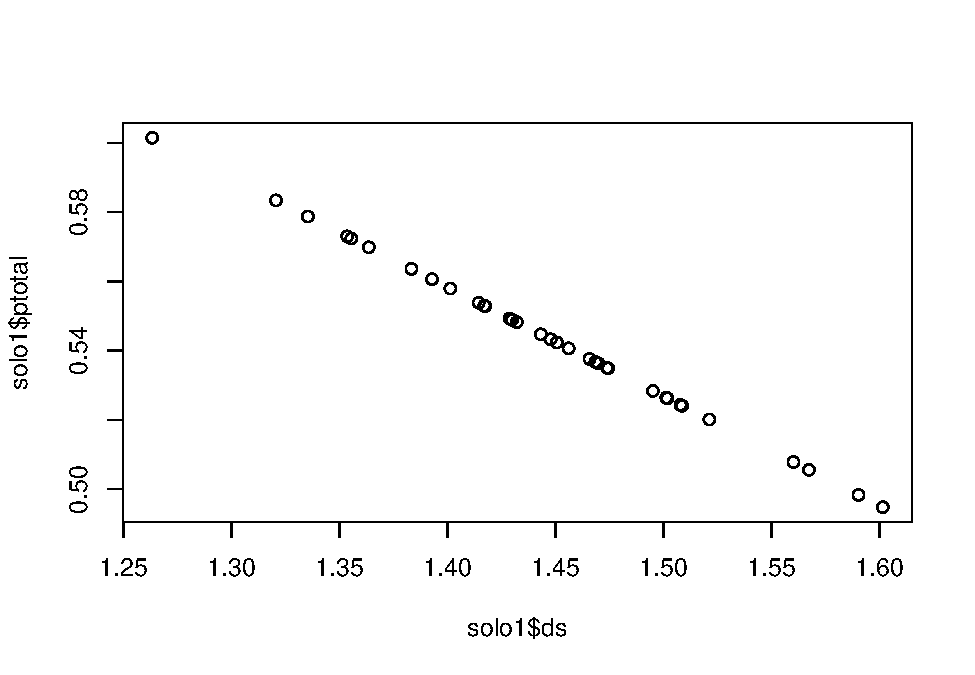
\includegraphics{TudodoR_files/figure-latex/unnamed-chunk-152-1.pdf}

Vamos no gráfico inserir linhas ligando os pontos. Use o argumento *type=``l'' na função \texttt{plot()}

\begin{Shaded}
\begin{Highlighting}[]
\KeywordTok{plot}\NormalTok{(solo1}\OperatorTok{$}\NormalTok{ds,solo1}\OperatorTok{$}\NormalTok{ptotal, }\DataTypeTok{type =} \StringTok{"l"}\NormalTok{)}
\end{Highlighting}
\end{Shaded}

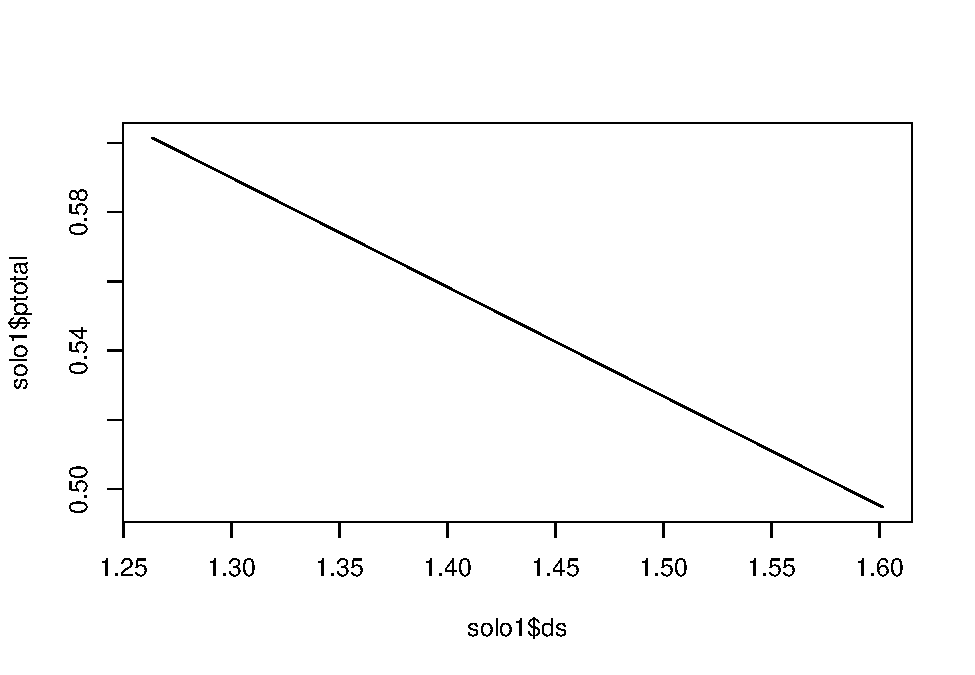
\includegraphics{TudodoR_files/figure-latex/unnamed-chunk-153-1.pdf}

Verifique outras opcões para os gráfico

\begin{itemize}
\tightlist
\item
  \emph{type = ``p''} especifica o tipo de plotagem
\item
  \emph{``p''}: pontos,
\item
  \emph{``l''}: linhas,
\item
  \emph{``b''}: pontos conectados por linhas,
\item
  \emph{``o''}: id. mas as linhas estão acima dos pontos,
\item
  \emph{``h''}: linhas verticais,
\item
  \emph{``s''}: passos, os dados são representados pelo topo das linhas verticais,
\item
  \emph{``S''}: id. mas os dados são representados pela parte inferior das linhas verticais
\end{itemize}

\begin{Shaded}
\begin{Highlighting}[]
\NormalTok{x <-}\StringTok{ }\DecValTok{0}\OperatorTok{:}\DecValTok{12}
\NormalTok{y <-}\StringTok{ }\KeywordTok{sin}\NormalTok{(pi}\OperatorTok{/}\DecValTok{5} \OperatorTok{*}\StringTok{ }\NormalTok{x)}
\NormalTok{op <-}\StringTok{ }\KeywordTok{par}\NormalTok{(}\DataTypeTok{mfrow =} \KeywordTok{c}\NormalTok{(}\DecValTok{3}\NormalTok{,}\DecValTok{3}\NormalTok{), }\DataTypeTok{mar =} \FloatTok{.1}\OperatorTok{+}\StringTok{ }\KeywordTok{c}\NormalTok{(}\DecValTok{2}\NormalTok{,}\DecValTok{2}\NormalTok{,}\DecValTok{3}\NormalTok{,}\DecValTok{1}\NormalTok{))}
\ControlFlowTok{for}\NormalTok{ (tp }\ControlFlowTok{in} \KeywordTok{c}\NormalTok{(}\StringTok{"p"}\NormalTok{,}\StringTok{"l"}\NormalTok{,}\StringTok{"b"}\NormalTok{,  }\StringTok{"c"}\NormalTok{,}\StringTok{"o"}\NormalTok{,}\StringTok{"h"}\NormalTok{,  }\StringTok{"s"}\NormalTok{,}\StringTok{"S"}\NormalTok{,}\StringTok{"n"}\NormalTok{)) \{}
  \KeywordTok{plot}\NormalTok{(y }\OperatorTok{~}\StringTok{ }\NormalTok{x, }\DataTypeTok{type =}\NormalTok{ tp, }\DataTypeTok{main =} \KeywordTok{paste0}\NormalTok{(}\StringTok{"plot(*, type = }\CharTok{\textbackslash{}"}\StringTok{"}\NormalTok{, tp, }\StringTok{"}\CharTok{\textbackslash{}"}\StringTok{)"}\NormalTok{))}
  \ControlFlowTok{if}\NormalTok{(tp }\OperatorTok{==}\StringTok{ "S"}\NormalTok{) \{}
    \KeywordTok{lines}\NormalTok{(x, y, }\DataTypeTok{type =} \StringTok{"s"}\NormalTok{, }\DataTypeTok{col =} \StringTok{"red"}\NormalTok{, }\DataTypeTok{lty =} \DecValTok{2}\NormalTok{)}
    \KeywordTok{mtext}\NormalTok{(}\StringTok{"lines(*, type = }\CharTok{\textbackslash{}"}\StringTok{s}\CharTok{\textbackslash{}"}\StringTok{, ...)"}\NormalTok{, }\DataTypeTok{col =} \StringTok{"red"}\NormalTok{, }\DataTypeTok{cex =} \FloatTok{0.8}\NormalTok{)}
\NormalTok{  \}}
\NormalTok{\}}
\end{Highlighting}
\end{Shaded}

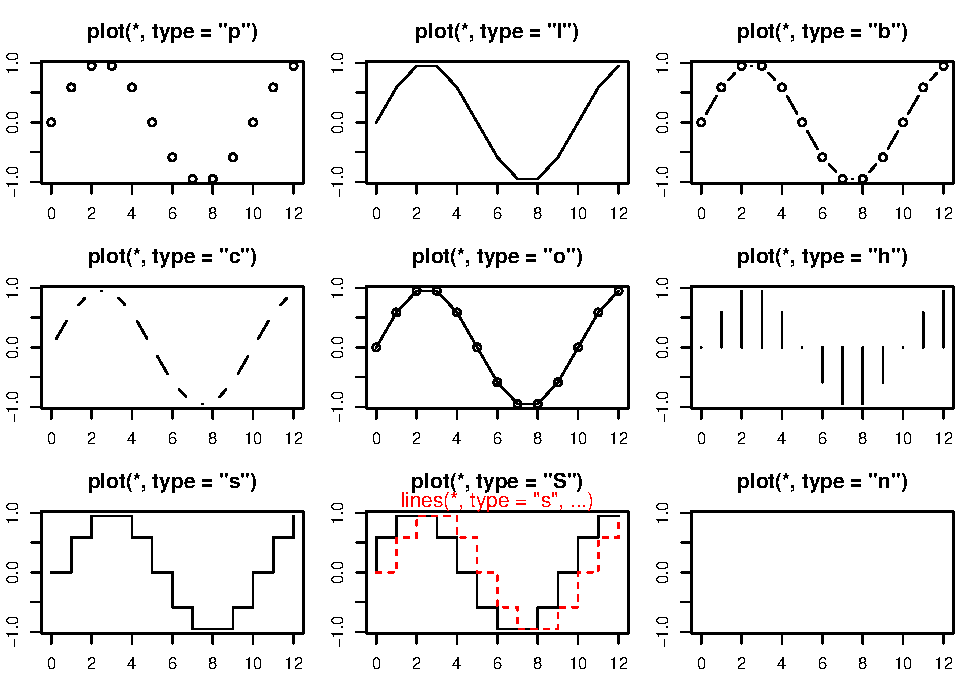
\includegraphics{TudodoR_files/figure-latex/unnamed-chunk-154-1.pdf}

\begin{Shaded}
\begin{Highlighting}[]
\KeywordTok{par}\NormalTok{(op)}
\end{Highlighting}
\end{Shaded}

\hypertarget{mudando-o-padrao-dos-pontos-pch}{%
\subsection{\texorpdfstring{Mudando o padrão dos pontos \texttt{pch=}}{Mudando o padrão dos pontos pch=}}\label{mudando-o-padrao-dos-pontos-pch}}

Pode-se usar diferentes padrões para os pontos usando o argumento \texttt{pch=}.Diferentes tipos de símbolos são associados a diferentes números. Pode-se ainda usar caracteres como o simbolo desejado.
Use a opção \texttt{pch\ =} para especificar simbolos a serem usados ao traçar pontos. Para os simbolos de 21 a 25, especifique a cor da borda \texttt{(col\ =)}.

\begin{Shaded}
\begin{Highlighting}[]
\KeywordTok{plot}\NormalTok{(solo1}\OperatorTok{$}\NormalTok{ds,solo1}\OperatorTok{$}\NormalTok{ptotal, }\DataTypeTok{pch=}\DecValTok{21}\NormalTok{, }\DataTypeTok{ylim =} \KeywordTok{c}\NormalTok{(}\DecValTok{0}\NormalTok{,}\FloatTok{0.6}\NormalTok{), }\DataTypeTok{xlim =} \KeywordTok{c}\NormalTok{(}\DecValTok{1}\NormalTok{,}\DecValTok{2}\NormalTok{))}
\end{Highlighting}
\end{Shaded}

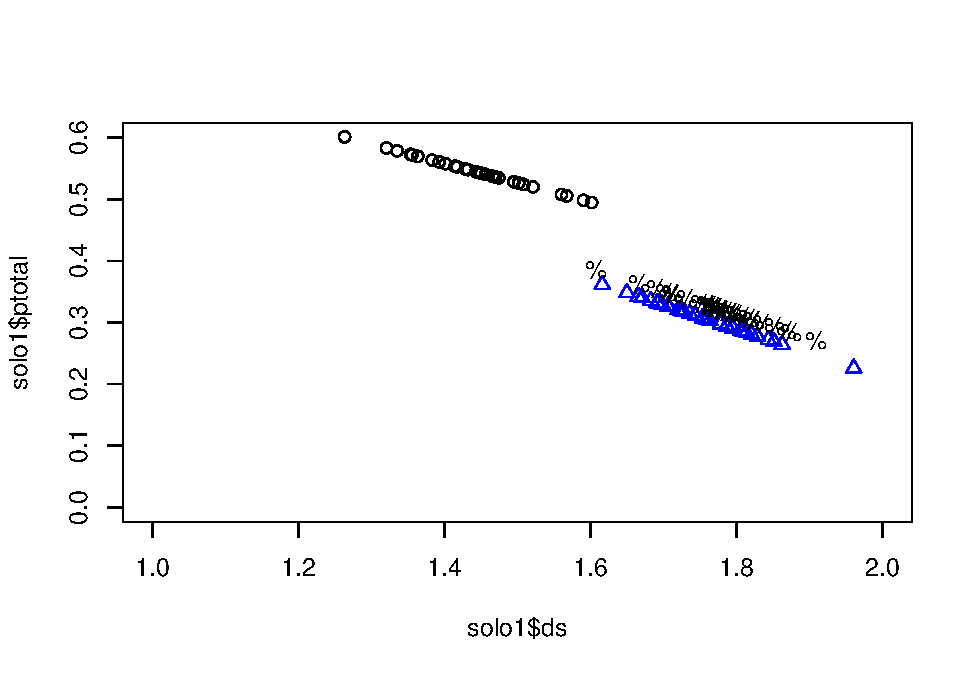
\includegraphics{TudodoR_files/figure-latex/unnamed-chunk-155-1.pdf}

\begin{Shaded}
\begin{Highlighting}[]
\KeywordTok{plot}\NormalTok{(solo2}\OperatorTok{$}\NormalTok{ds,solo2}\OperatorTok{$}\NormalTok{ptotal,}\DataTypeTok{pch=}\DecValTok{2}\NormalTok{, }\DataTypeTok{col=}\StringTok{"blue"}\NormalTok{) }
\end{Highlighting}
\end{Shaded}

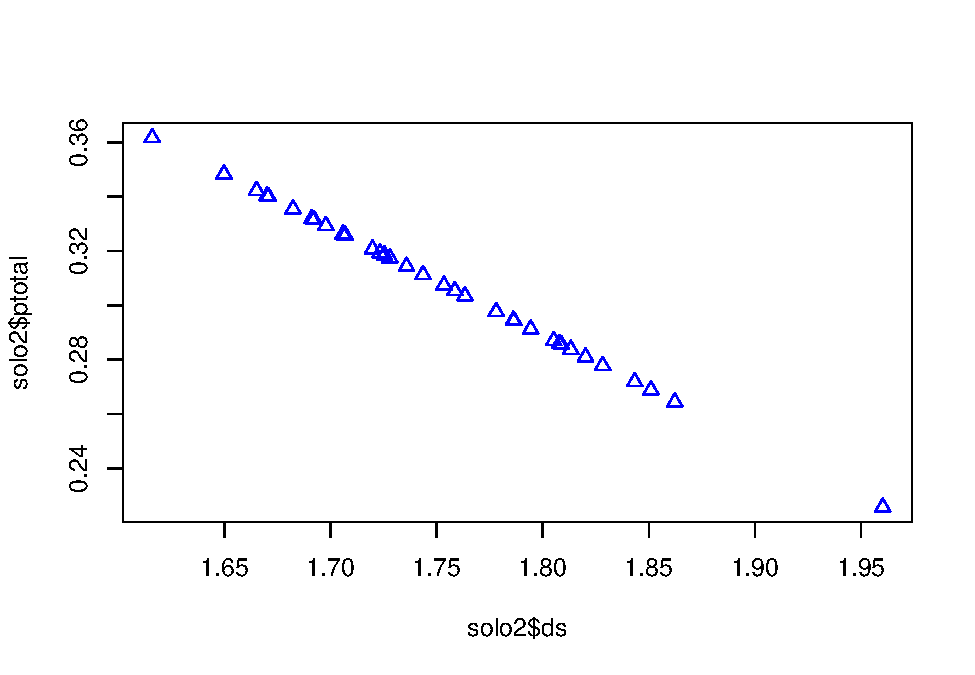
\includegraphics{TudodoR_files/figure-latex/unnamed-chunk-155-2.pdf}

\begin{Shaded}
\begin{Highlighting}[]
\KeywordTok{plot}\NormalTok{(solo3}\OperatorTok{$}\NormalTok{ds,solo3}\OperatorTok{$}\NormalTok{ptotal,}\DataTypeTok{pch=}\StringTok{"%"}\NormalTok{)}
\end{Highlighting}
\end{Shaded}

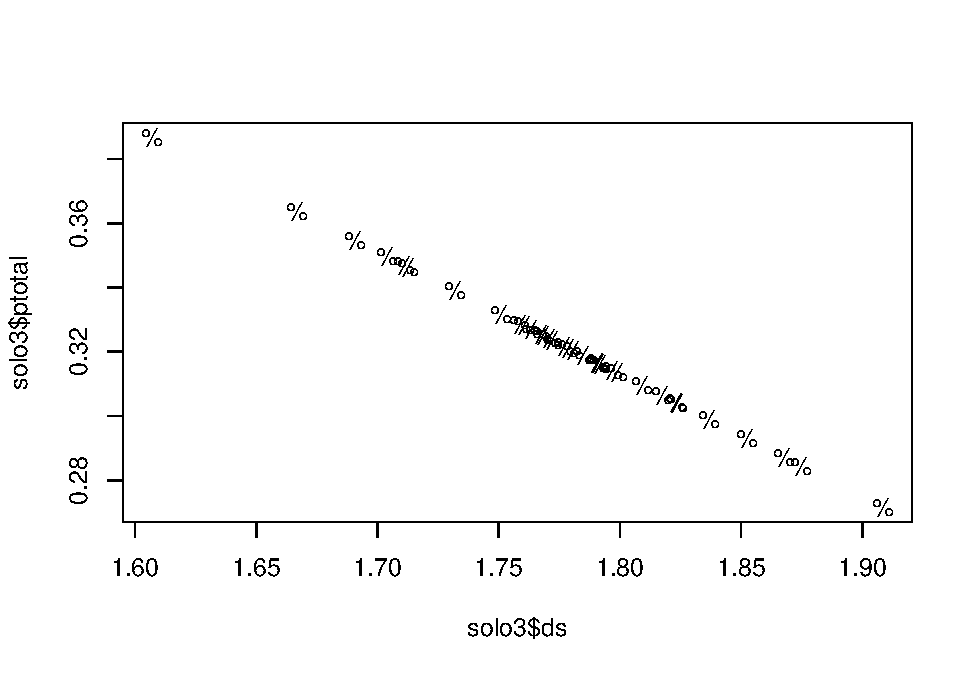
\includegraphics{TudodoR_files/figure-latex/unnamed-chunk-155-3.pdf}

Neste exemplo acima note, que foi adicionado o argumento \texttt{ylim} e \texttt{xlim} eles limitam os valores minimos e maximos:

\begin{Shaded}
\begin{Highlighting}[]
\NormalTok{xlim=}\KeywordTok{c}\NormalTok{(xmin, xmax) ylim=}\KeywordTok{c}\NormalTok{(ymin, ymax)}\ErrorTok{)}
\end{Highlighting}
\end{Shaded}

Veja um exemplo do padrão dos pontos.

\begin{Shaded}
\begin{Highlighting}[]
\KeywordTok{plot}\NormalTok{ (}\DecValTok{0}\OperatorTok{:}\DecValTok{20}\NormalTok{,                         }\CommentTok{#coord. eixo X}
      \KeywordTok{rep}\NormalTok{ (}\DecValTok{0}\NormalTok{,}\DecValTok{21}\NormalTok{),                   }\CommentTok{#coord. eixo y}
      \DataTypeTok{pch =} \DecValTok{0}\OperatorTok{:}\DecValTok{20}\NormalTok{,                   }\CommentTok{#padrão dos pontos variando}
      \DataTypeTok{cex =} \DecValTok{2}\NormalTok{,                      }\CommentTok{#tamanho dos pontos}
      \DataTypeTok{main =} \StringTok{"Padrão dos pontos"}\NormalTok{, }\CommentTok{#Titulo (note o \textbackslash{}n)}
      \DataTypeTok{xlab =} \StringTok{"pch = "}\NormalTok{,              }\CommentTok{#texto do eixo de x}
      \DataTypeTok{ylab =} \StringTok{""}\NormalTok{)                    }\CommentTok{#texto do eixo de y}
\end{Highlighting}
\end{Shaded}

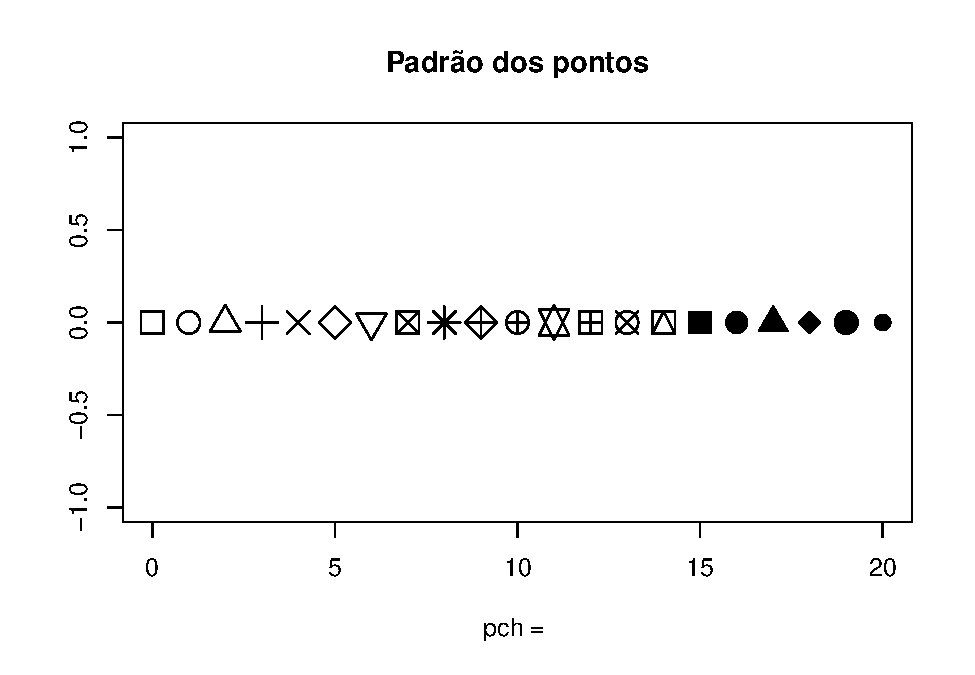
\includegraphics{TudodoR_files/figure-latex/unnamed-chunk-157-1.pdf}

\hypertarget{mudando-as-linhas-lwd-e-lty}{%
\subsection{\texorpdfstring{Mudando as linhas (\texttt{lwd\ e\ lty})}{Mudando as linhas (lwd e lty)}}\label{mudando-as-linhas-lwd-e-lty}}

Você pode alterar linhas usando as seguintes opções. Isso é particularmente útil para linhas de referência, eixos e linhas de ajuste. A largura das linhas pode ser mudada com o argumento \texttt{lwd=}, enquanto os estilos das linhas podem ser modificados com o argumento \texttt{lty=}.

\begin{Shaded}
\begin{Highlighting}[]
\KeywordTok{plot}\NormalTok{(solo3}\OperatorTok{$}\NormalTok{ds,solo3}\OperatorTok{$}\NormalTok{ptotal, }\DataTypeTok{lwd=}\DecValTok{2}\NormalTok{) }\CommentTok{# linha grossa}
\end{Highlighting}
\end{Shaded}

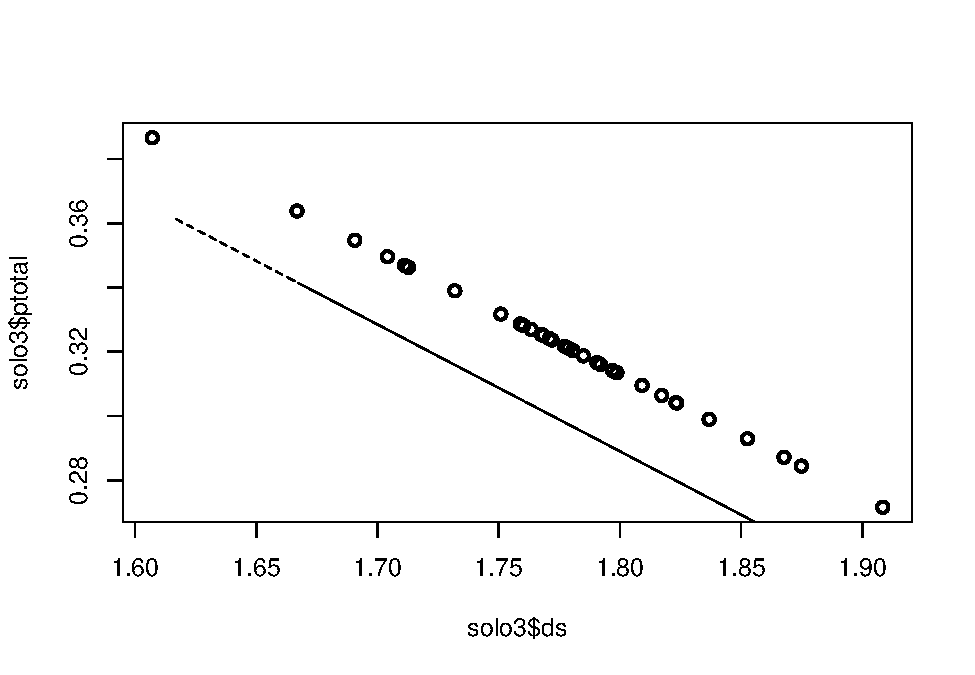
\includegraphics{TudodoR_files/figure-latex/unnamed-chunk-158-1.pdf}

\begin{Shaded}
\begin{Highlighting}[]
\KeywordTok{plot}\NormalTok{(solo2}\OperatorTok{$}\NormalTok{ds,solo2}\OperatorTok{$}\NormalTok{ptotal, }\DataTypeTok{lty=}\DecValTok{2}\NormalTok{) }\CommentTok{#linha interrompida}
\end{Highlighting}
\end{Shaded}

\includegraphics{TudodoR_files/figure-latex/unnamed-chunk-158-2.pdf}

\begin{Shaded}
\begin{Highlighting}[]
\NormalTok{x <-}\StringTok{ }\DecValTok{1}\OperatorTok{:}\DecValTok{9}
\NormalTok{y <-}\StringTok{ }\DecValTok{1}\OperatorTok{:}\DecValTok{9}
  \KeywordTok{plot}\NormalTok{(x, y, }\DataTypeTok{type =} \StringTok{"n"}\NormalTok{)}
    \KeywordTok{lines}\NormalTok{(}\KeywordTok{c}\NormalTok{(}\DecValTok{2}\NormalTok{, }\DecValTok{8}\NormalTok{), }\KeywordTok{c}\NormalTok{(}\DecValTok{8}\NormalTok{, }\DecValTok{8}\NormalTok{), }\DataTypeTok{lwd =} \DecValTok{2}\NormalTok{)}
    \KeywordTok{lines}\NormalTok{(}\KeywordTok{c}\NormalTok{(}\DecValTok{2}\NormalTok{, }\DecValTok{8}\NormalTok{), }\KeywordTok{c}\NormalTok{(}\DecValTok{7}\NormalTok{, }\DecValTok{7}\NormalTok{), }\DataTypeTok{lty =} \DecValTok{2}\NormalTok{, }\DataTypeTok{lwd =} \DecValTok{2}\NormalTok{)}
    \KeywordTok{lines}\NormalTok{(}\KeywordTok{c}\NormalTok{(}\DecValTok{2}\NormalTok{, }\DecValTok{8}\NormalTok{), }\KeywordTok{c}\NormalTok{(}\DecValTok{6}\NormalTok{, }\DecValTok{6}\NormalTok{), }\DataTypeTok{lty =} \DecValTok{3}\NormalTok{, }\DataTypeTok{lwd =} \DecValTok{2}\NormalTok{)}
    \KeywordTok{lines}\NormalTok{(}\KeywordTok{c}\NormalTok{(}\DecValTok{2}\NormalTok{, }\DecValTok{8}\NormalTok{), }\KeywordTok{c}\NormalTok{(}\DecValTok{5}\NormalTok{, }\DecValTok{5}\NormalTok{), }\DataTypeTok{lty =} \DecValTok{4}\NormalTok{, }\DataTypeTok{lwd =} \DecValTok{2}\NormalTok{)}
    \KeywordTok{lines}\NormalTok{(}\KeywordTok{c}\NormalTok{(}\DecValTok{2}\NormalTok{, }\DecValTok{8}\NormalTok{), }\KeywordTok{c}\NormalTok{(}\DecValTok{4}\NormalTok{, }\DecValTok{4}\NormalTok{), }\DataTypeTok{lty =} \DecValTok{5}\NormalTok{, }\DataTypeTok{lwd =} \DecValTok{2}\NormalTok{)}
    \KeywordTok{lines}\NormalTok{(}\KeywordTok{c}\NormalTok{(}\DecValTok{2}\NormalTok{, }\DecValTok{8}\NormalTok{), }\KeywordTok{c}\NormalTok{(}\DecValTok{3}\NormalTok{, }\DecValTok{3}\NormalTok{), }\DataTypeTok{lty =} \DecValTok{6}\NormalTok{, }\DataTypeTok{lwd =} \DecValTok{2}\NormalTok{)}
\end{Highlighting}
\end{Shaded}

\includegraphics{TudodoR_files/figure-latex/unnamed-chunk-159-1.pdf}

\hypertarget{adicionando-linhas-a-um-grafico-de-pontos}{%
\subsection{Adicionando linhas a um grafico de pontos}\label{adicionando-linhas-a-um-grafico-de-pontos}}

A função utilizada para inserir linhas é \texttt{abline()}.
Vamos usar a função \texttt{abline} para inserir uma linha que mostra a média dos dados do eixo Y.
o h é de linha horizontal. Fará uma linha na horizontal que passa pela média de y.

\begin{Shaded}
\begin{Highlighting}[]
\KeywordTok{plot}\NormalTok{(solo3}\OperatorTok{$}\NormalTok{ds,solo3}\OperatorTok{$}\NormalTok{ptotal, }\KeywordTok{abline}\NormalTok{(}\DataTypeTok{h=}\KeywordTok{mean}\NormalTok{(solo3}\OperatorTok{$}\NormalTok{ptotal))) }
\end{Highlighting}
\end{Shaded}

\includegraphics{TudodoR_files/figure-latex/unnamed-chunk-160-1.pdf}

Para passar uma linha que passa pela média de x

\begin{Shaded}
\begin{Highlighting}[]
\KeywordTok{plot}\NormalTok{(solo3}\OperatorTok{$}\NormalTok{ds,solo3}\OperatorTok{$}\NormalTok{ptotal)}
\end{Highlighting}
\end{Shaded}

\includegraphics{TudodoR_files/figure-latex/unnamed-chunk-161-1.pdf}

\begin{Shaded}
\begin{Highlighting}[]
\KeywordTok{plot}\NormalTok{(solo3}\OperatorTok{$}\NormalTok{ds,solo3}\OperatorTok{$}\NormalTok{ptotal, }\KeywordTok{abline}\NormalTok{(}\DataTypeTok{v=}\KeywordTok{mean}\NormalTok{(solo3}\OperatorTok{$}\NormalTok{ds))) }\CommentTok{## o v é de vertical}
\end{Highlighting}
\end{Shaded}

\includegraphics{TudodoR_files/figure-latex/unnamed-chunk-162-1.pdf}

Também é possível inserir as duas linhas ao mesmo tempo.

\begin{Shaded}
\begin{Highlighting}[]
\KeywordTok{plot}\NormalTok{(solo3}\OperatorTok{$}\NormalTok{ds,solo3}\OperatorTok{$}\NormalTok{ptotal, }\KeywordTok{abline}\NormalTok{(}\DataTypeTok{h=}\KeywordTok{mean}\NormalTok{(solo3}\OperatorTok{$}\NormalTok{ptotal), }\DataTypeTok{v=}\KeywordTok{mean}\NormalTok{(solo3}\OperatorTok{$}\NormalTok{ds),}\DataTypeTok{col=}\StringTok{"red"}\NormalTok{))}
\end{Highlighting}
\end{Shaded}

\includegraphics{TudodoR_files/figure-latex/unnamed-chunk-163-1.pdf}

Com cores diferentes

\begin{Shaded}
\begin{Highlighting}[]
\KeywordTok{plot}\NormalTok{(solo3}\OperatorTok{$}\NormalTok{ds,solo3}\OperatorTok{$}\NormalTok{ptotal, }\KeywordTok{abline}\NormalTok{(}\DataTypeTok{h=}\KeywordTok{mean}\NormalTok{(solo3}\OperatorTok{$}\NormalTok{ptotal), }\DataTypeTok{v=}\KeywordTok{mean}\NormalTok{(solo3}\OperatorTok{$}\NormalTok{ds),}\DataTypeTok{col=}\KeywordTok{c}\NormalTok{(}\DecValTok{2}\NormalTok{,}\DecValTok{4}\NormalTok{)))}
\end{Highlighting}
\end{Shaded}

\includegraphics{TudodoR_files/figure-latex/unnamed-chunk-164-1.pdf}

\hypertarget{definindo-o-intervalo-dos-eixos}{%
\subsection{Definindo o intervalo dos eixos}\label{definindo-o-intervalo-dos-eixos}}

Se você quiser preencher um mesmo gráfico com linhas e pontos que possuem diferentes amplitudes como nosso exemplo do solos, deve usar o argumento \texttt{type=n}. Com este argumento um gráfico em branco é criado.

\begin{Shaded}
\begin{Highlighting}[]
\KeywordTok{plot}\NormalTok{(}\KeywordTok{c}\NormalTok{(}\FloatTok{1.55}\NormalTok{,}\DecValTok{2}\NormalTok{),}\KeywordTok{c}\NormalTok{(}\DecValTok{0}\NormalTok{,}\FloatTok{0.6}\NormalTok{),}\DataTypeTok{type=}\StringTok{'n'}\NormalTok{)}
\KeywordTok{points}\NormalTok{(solo3}\OperatorTok{$}\NormalTok{ds,solo3}\OperatorTok{$}\NormalTok{ptotal, }\DataTypeTok{pch=}\DecValTok{2}\NormalTok{)}
\KeywordTok{points}\NormalTok{(solo2}\OperatorTok{$}\NormalTok{ds,solo2}\OperatorTok{$}\NormalTok{ptotal)}
\end{Highlighting}
\end{Shaded}

\includegraphics{TudodoR_files/figure-latex/unnamed-chunk-165-1.pdf}

\hypertarget{personalizando-os-graficos}{%
\subsection{Personalizando os gráficos}\label{personalizando-os-graficos}}

Alguns parâmetros podem ser usados no intuito de personalizar um gráfico no R.

Exemplo:

\begin{Shaded}
\begin{Highlighting}[]
\KeywordTok{plot}\NormalTok{(solo1}\OperatorTok{$}\NormalTok{ptotal,solo1}\OperatorTok{$}\NormalTok{ds)}
\end{Highlighting}
\end{Shaded}

\includegraphics{TudodoR_files/figure-latex/unnamed-chunk-166-1.pdf}

\begin{Shaded}
\begin{Highlighting}[]
\KeywordTok{plot}\NormalTok{(solo1}\OperatorTok{$}\NormalTok{ptotal,solo1}\OperatorTok{$}\NormalTok{ds,          }\CommentTok{#plota ds e ptotal}
\DataTypeTok{xlab=}\StringTok{"Macroporosdiade (%)"}\NormalTok{,          }\CommentTok{#nomeia o eixo x}
\DataTypeTok{ylab=}\KeywordTok{expression}\NormalTok{(Ds}\OperatorTok{~}\NormalTok{(mg}\OperatorTok{~}\NormalTok{Kg}\OperatorTok{^}\NormalTok{\{}\OperatorTok{-}\DecValTok{1}\NormalTok{\})),    }\CommentTok{#nomeia o eixo y}
\DataTypeTok{main=}\StringTok{"Como personalizar um gráfico"}\NormalTok{, }\CommentTok{#referente ao título}
\DataTypeTok{xlim=}\KeywordTok{c}\NormalTok{(}\FloatTok{0.48}\NormalTok{,}\FloatTok{0.64}\NormalTok{),                   }\CommentTok{#limites do eixo x}
\DataTypeTok{ylim=}\KeywordTok{c}\NormalTok{(}\DecValTok{0}\NormalTok{,}\DecValTok{2}\NormalTok{), }\DataTypeTok{col=}\StringTok{"red"}\NormalTok{,              }\CommentTok{#limites do eixo y}
\DataTypeTok{pch=}\DecValTok{22}\NormalTok{,                              }\CommentTok{#padrão dos pontos}
\DataTypeTok{bg=}\StringTok{"yellow"}\NormalTok{,                         }\CommentTok{#cor de preenchimento}
\DataTypeTok{tcl=}\FloatTok{0.4}\NormalTok{,                             }\CommentTok{#tamanho dos traços dos eixos}
\DataTypeTok{las=}\DecValTok{1}\NormalTok{,                               }\CommentTok{#orientação do texto em y}
\DataTypeTok{cex=}\FloatTok{1.5}\NormalTok{,                             }\CommentTok{#tamanho do objeto do ponto}
\DataTypeTok{bty=}\StringTok{"l"}\NormalTok{,                             }\CommentTok{#altera as bordas}
\KeywordTok{abline}\NormalTok{(}\KeywordTok{lm}\NormalTok{(solo1}\OperatorTok{$}\NormalTok{ds}\OperatorTok{~}\NormalTok{solo1}\OperatorTok{$}\NormalTok{ptotal)))   }\CommentTok{#regressao dos pontos}
\end{Highlighting}
\end{Shaded}

\includegraphics{TudodoR_files/figure-latex/unnamed-chunk-166-2.pdf}

Veja o \texttt{demo(plotmath)} para saber mais sobre anotações em gráficos.

\hypertarget{histogramas}{%
\section{Histogramas}\label{histogramas}}

A função \texttt{hist()} produz um histograma dos dados informados em seu argumento enquanto a função \texttt{barplot()} produz um gráfico de barras.

\begin{Shaded}
\begin{Highlighting}[]
\KeywordTok{hist}\NormalTok{(solo1}\OperatorTok{$}\NormalTok{ds)}
\KeywordTok{rug}\NormalTok{(solo1}\OperatorTok{$}\NormalTok{ds)}
\end{Highlighting}
\end{Shaded}

\includegraphics{TudodoR_files/figure-latex/unnamed-chunk-167-1.pdf}

\hypertarget{personalizando-graficos}{%
\subsection{Personalizando gráficos}\label{personalizando-graficos}}

Os histogramas criados no R seguem um certo padrão (conhecido como parâmetros
default) que podem ser alterados de acordo com a preferência do usuário. Você pode obter
informações detalhadas desses parâmetros se usar os recursos de ajuda do R.

\begin{Shaded}
\begin{Highlighting}[]
\KeywordTok{hist}\NormalTok{(solo1}\OperatorTok{$}\NormalTok{ds, }\CommentTok{#histograma de ds}
     \DataTypeTok{main=}\StringTok{"Histograma Personalizado}\CharTok{\textbackslash{}n}\StringTok{densidade do solo"}\NormalTok{,}\CommentTok{#título}
     \DataTypeTok{xlab=}\KeywordTok{expression}\NormalTok{(Ds}\OperatorTok{~}\NormalTok{(mg}\OperatorTok{~}\NormalTok{Kg}\OperatorTok{^}\NormalTok{\{}\OperatorTok{-}\DecValTok{1}\NormalTok{\})), }\CommentTok{#texto do eixo das abscissas}
     \DataTypeTok{ylab=}\StringTok{"Probabilidades"}\NormalTok{, }\CommentTok{#texto do eixo das ordenadas}
     \DataTypeTok{xlim=}\KeywordTok{c}\NormalTok{(}\DecValTok{1}\NormalTok{,}\DecValTok{2}\NormalTok{), }\CommentTok{#limites do eixo de x}
     \DataTypeTok{ylim=}\KeywordTok{c}\NormalTok{(}\DecValTok{0}\NormalTok{,}\DecValTok{10}\NormalTok{), }\CommentTok{#limites do eixo y}
     \DataTypeTok{col=}\StringTok{"lightblue"}\NormalTok{, }\CommentTok{#cor das colunas}
     \DataTypeTok{border=}\StringTok{"white"}\NormalTok{, }\CommentTok{#cor das bordas das colunas}
     \DataTypeTok{adj=}\DecValTok{0}\NormalTok{, }\CommentTok{#alinhamento dos textos 0, 0.5 e 1}
     \DataTypeTok{col.axis=}\StringTok{"red"}\NormalTok{) }\CommentTok{#cor do texto nos eixos}
\end{Highlighting}
\end{Shaded}

\includegraphics{TudodoR_files/figure-latex/unnamed-chunk-168-1.pdf}

\hypertarget{graficos-de-barras}{%
\section{Gráficos de Barras}\label{graficos-de-barras}}

Assemelha-se ao histograma, Porém, nesse caso, os dados referem-se a categoria ou aos tratamentos

\begin{Shaded}
\begin{Highlighting}[]
\KeywordTok{barplot}\NormalTok{(solo}\OperatorTok{$}\NormalTok{ptotal,}\DataTypeTok{names.arg=}\NormalTok{solo}\OperatorTok{$}\NormalTok{z, }\DataTypeTok{horiz =}\NormalTok{ T)}
\end{Highlighting}
\end{Shaded}

\includegraphics{TudodoR_files/figure-latex/unnamed-chunk-169-1.pdf}

\hypertarget{boxplots}{%
\section{Boxplots}\label{boxplots}}

Dados de um experimento visando controle de pulgão (\emph{Aphis gossypii Glover}) em cultura de pepino, instalado em \emph{delineamento inteiramente casualizado} com 6 repetições. A resposta observada foi o número de pulgões após a aplicação de produtos indicados para seu controle.

\begin{Shaded}
\begin{Highlighting}[]
\NormalTok{dados <-}\StringTok{ }\KeywordTok{read.table}\NormalTok{(}\StringTok{"https://www.dropbox.com/s/jjyo8dhyy0qt3ft/BanzattoQd3.2.1.txt?dl=1"}\NormalTok{)}
\KeywordTok{str}\NormalTok{(dados)}
\end{Highlighting}
\end{Shaded}

\begin{verbatim}
## 'data.frame':    30 obs. of  3 variables:
##  $ trat   : Factor w/ 5 levels "Azinfos etilico",..: 5 1 3 4 2 5 1 3 4 2 ...
##  $ rept   : int  1 1 1 1 1 2 2 2 2 2 ...
##  $ pulgoes: int  2370 1282 562 173 193 1687 1527 321 127 71 ...
\end{verbatim}

\emph{trat}
Fator de níveis nominais. Tratamento aplicado para controle do pulgão.

\emph{rept}
Número inteiro que identifica as repetições de cada tratamento.

\emph{pulgões}
Número de pulgões coletados 36 horas após a pulverização dos tratamentos.

Boxplots podem ser criados para variáveis individuais ou para variáveis por grupo. O formato é \texttt{boxplot} \texttt{(\ x\ ,\ data\ =)} , em que \texttt{x} é uma fórmula e \texttt{data\ =} denota o quadro de dados que fornece os dados.

Um exemplo de uma fórmula é \texttt{y\ \textasciitilde{}\ group} onde um boxplot separado para a variável numérica é gerado para cada valor de group.

\begin{Shaded}
\begin{Highlighting}[]
\KeywordTok{x11}\NormalTok{()}
\KeywordTok{boxplot}\NormalTok{(pulgoes}\OperatorTok{~}\NormalTok{trat,              }\CommentTok{#formula do boxplot}
        \DataTypeTok{data =}\NormalTok{ dados,              }\CommentTok{#conjunto de dados}
        \DataTypeTok{main=}\StringTok{"boxplot"}\NormalTok{,            }\CommentTok{#título}
        \DataTypeTok{xlab=}\StringTok{"Controle do pulgão"}\NormalTok{, }\CommentTok{#texto do eixo x }
        \DataTypeTok{ylab=}\StringTok{"Numero de plugões",  #texto do eixo y}
\StringTok{        col=3)                     #cor verde  }
\end{Highlighting}
\end{Shaded}

\includegraphics{TudodoR_files/figure-latex/unnamed-chunk-171-1.pdf}

Adicione \texttt{horizontal\ =\ TRUE} para inverter a orientação do eixo.

\begin{Shaded}
\begin{Highlighting}[]
\KeywordTok{boxplot}\NormalTok{(pulgoes}\OperatorTok{~}\NormalTok{trat,              }\CommentTok{#formula do boxplot}
        \DataTypeTok{data =}\NormalTok{ dados,              }\CommentTok{#conjunto de dados}
        \DataTypeTok{main=}\StringTok{"boxplot"}\NormalTok{,            }\CommentTok{#t?tulo}
        \DataTypeTok{xlab=}\StringTok{"Controle do pulgão"}\NormalTok{, }\CommentTok{#texto do eixo x }
        \DataTypeTok{ylab=}\StringTok{"Numero de plugões",  #texto do eixo y}
\StringTok{        col=3, horizontal = T,     #cor verde  }
\StringTok{        notch=T)                   #teste para mediana}
\end{Highlighting}
\end{Shaded}

\begin{verbatim}
## Warning in bxp(list(stats = structure(c(825, 871, 972.5, 1282, 1527, 44, :
## some notches went outside hinges ('box'): maybe set notch=FALSE
\end{verbatim}

\includegraphics{TudodoR_files/figure-latex/unnamed-chunk-172-1.pdf}

\hypertarget{boxplot-com-fatorial}{%
\subsection{Boxplot com fatorial}\label{boxplot-com-fatorial}}

Boxplot com 2 fatores, com caixas coloridas para facilitar a interpretação.

\textbf{Efeito de Recipientes para duas Espécies de Eucalipto}

Experimento em esquema fatorial 3x2 para estudar o efeito de 3 tipos de recipientes para a produção de mudas de duas espécies de Eucalipto. O experimento foi instalado em delineamento inteiramente casualizado.

\emph{recipie}
São os níveis de recipiente estudados:
- SPP - saco plástico pequeno;
- SPG - saco plástico grande; e
- Lam - laminado.

\emph{especie}
São as espécies de Eucalipto: \emph{Eucalyptus citriodora} e \emph{Eucalyptus grandis}

\emph{rept}
Identifica as repetições de cada combinação dos fatores recipiente e espécie.

\emph{alt}
Altura das mudas aos 80 dias de idade (cm).

Baixar dados via web.

\begin{Shaded}
\begin{Highlighting}[]
\NormalTok{fat <-}\StringTok{ }\KeywordTok{read.table}\NormalTok{(}\StringTok{"https://www.dropbox.com/s/sahc5n80rlkcfx4/BanzattoQd5.2.4.txt?dl=1"}\NormalTok{)}
\KeywordTok{str}\NormalTok{(fat)}
\end{Highlighting}
\end{Shaded}

\begin{verbatim}
## 'data.frame':    24 obs. of  4 variables:
##  $ recipie: Factor w/ 3 levels "Lam","SPG","SPP": 3 3 2 2 1 1 3 3 2 2 ...
##  $ especie: Factor w/ 2 levels "E. citriodora",..: 1 2 1 2 1 2 1 2 1 2 ...
##  $ rept   : int  1 1 1 1 1 1 2 2 2 2 ...
##  $ alt    : num  26.2 24.8 25.7 19.6 22.8 19.8 26 24.6 26.3 21.1 ...
\end{verbatim}

Gerar o gráfico boxpolt com o comando abaixo.

\begin{Shaded}
\begin{Highlighting}[]
\KeywordTok{boxplot}\NormalTok{(fat}\OperatorTok{$}\NormalTok{alt}\OperatorTok{~}\NormalTok{fat}\OperatorTok{$}\NormalTok{recipie}\OperatorTok{*}\NormalTok{especie, }\DataTypeTok{data=}\NormalTok{fat, }\DataTypeTok{notch=}\NormalTok{F, }
        \DataTypeTok{col=}\NormalTok{(}\KeywordTok{c}\NormalTok{(}\StringTok{"gold"}\NormalTok{,}\StringTok{"darkgreen"}\NormalTok{,}\StringTok{"brown"}\NormalTok{)),}
        \DataTypeTok{main=}\StringTok{"Fatorial"}\NormalTok{, }\DataTypeTok{xlab=}\StringTok{"Recipiente e Espécies"}\NormalTok{,}
        \DataTypeTok{ylab=}\StringTok{"Altura de plantas (cm)"}\NormalTok{)}
\end{Highlighting}
\end{Shaded}

\includegraphics{TudodoR_files/figure-latex/unnamed-chunk-174-1.pdf}

\hypertarget{cores}{%
\section{Cores}\label{cores}}

Gráficos em preto e branco são bons na maioria dos casos, mas cores podem ser mudadas usando \texttt{col="red"} (escrevendo o nome da cor) ou \texttt{col=2} (usando números).
O comando abaixo mostra os números que especificam algumas cores.

\begin{Shaded}
\begin{Highlighting}[]
\KeywordTok{pie}\NormalTok{(}\KeywordTok{rep}\NormalTok{(}\DecValTok{1}\NormalTok{,}\DecValTok{30}\NormalTok{),}\DataTypeTok{col=}\KeywordTok{rainbow}\NormalTok{(}\DecValTok{30}\NormalTok{))}
\end{Highlighting}
\end{Shaded}

\includegraphics{TudodoR_files/figure-latex/unnamed-chunk-175-1.pdf}

Veja sua tabela de cores executando o script \href{https://www.dropbox.com/s/e9a27z97buqjovz/paletadecores.R?dl=1}{paletedecores.R}.

Podemos também criar cores personalizadas usando a função do \texttt{rgb()}, que recebe como argumentos as quantidades de vermelho \emph{(red)}, verde \emph{(green)} e azul \emph{(blue)} e, opcionalmente, o grau de opacidade (alpha). Os valores devem ser números reais entre 0 e 1.

Exemplos:

\begin{Shaded}
\begin{Highlighting}[]
\NormalTok{goiaba <-}\StringTok{ }\KeywordTok{rgb}\NormalTok{(}\FloatTok{0.94}\NormalTok{, }\FloatTok{0.41}\NormalTok{, }\FloatTok{0.40}\NormalTok{)}
\NormalTok{goiaba.semitrans <-}\StringTok{ }\KeywordTok{rgb}\NormalTok{(}\FloatTok{0.94}\NormalTok{, }\FloatTok{0.41}\NormalTok{, }\FloatTok{0.40}\NormalTok{, }\DataTypeTok{alpha =} \FloatTok{0.5}\NormalTok{)}
\NormalTok{vitamina <-}\StringTok{ }\KeywordTok{rgb}\NormalTok{(}\DataTypeTok{red =} \KeywordTok{c}\NormalTok{(}\FloatTok{0.87}\NormalTok{, }\FloatTok{0.70}\NormalTok{), }\DataTypeTok{green =} \KeywordTok{c}\NormalTok{(}\FloatTok{0.83}\NormalTok{, }\FloatTok{0.77}\NormalTok{),}
\DataTypeTok{blue =} \KeywordTok{c}\NormalTok{(}\FloatTok{0.71}\NormalTok{, }\FloatTok{0.30}\NormalTok{), }\DataTypeTok{names =} \KeywordTok{c}\NormalTok{(}\StringTok{"leite"}\NormalTok{, }\StringTok{"abacate"}\NormalTok{))}
\end{Highlighting}
\end{Shaded}

\hypertarget{interagindo-com-a-janela-grafica}{%
\section{Interagindo com a Janela gráfica}\label{interagindo-com-a-janela-grafica}}

Poderemos com o mouse marcar o ponte desejado usando a função \texttt{identify\ ()}

\begin{Shaded}
\begin{Highlighting}[]
\KeywordTok{plot}\NormalTok{(solo1}\OperatorTok{$}\NormalTok{ds}\OperatorTok{~}\NormalTok{solo1}\OperatorTok{$}\NormalTok{ptotal)}
\KeywordTok{identify}\NormalTok{(solo1}\OperatorTok{$}\NormalTok{ds,}\DataTypeTok{n=}\DecValTok{1}\NormalTok{)}
\end{Highlighting}
\end{Shaded}

\includegraphics{TudodoR_files/figure-latex/unnamed-chunk-177-1.pdf}

\begin{verbatim}
## integer(0)
\end{verbatim}

\hypertarget{texto-e-tamanho-do-simbolo}{%
\section{Texto e tamanho do símbolo}\label{texto-e-tamanho-do-simbolo}}

As seguintes opções podem ser usadas para controlar o tamanho do texto e do símbolo em gráficos.

\texttt{cex} número que indica o valor pelo qual o texto e os símbolos de plotagem devem ser dimensionados em relação ao padrão.
\emph{1 = padrão, 1,5 é 50\% maior, 0,5 é 50\% menor, etc.}

\hypertarget{visualizar-varios-graficos}{%
\section{Visualizar vários gráficos}\label{visualizar-varios-graficos}}

\begin{Shaded}
\begin{Highlighting}[]
\KeywordTok{x11}\NormalTok{()}
\KeywordTok{boxplot}\NormalTok{(pulgoes}\OperatorTok{~}\NormalTok{trat,              }\CommentTok{#formula do boxplot}
        \DataTypeTok{data =}\NormalTok{ dados,              }\CommentTok{#conjunto de dados}
        \DataTypeTok{main=}\StringTok{"boxplot"}\NormalTok{,            }\CommentTok{#título}
        \DataTypeTok{xlab=}\StringTok{"Controle do pulgão"}\NormalTok{, }\CommentTok{#texto do eixo x }
        \DataTypeTok{ylab=}\StringTok{"Numero de plugões",  #texto do eixo y}
\StringTok{        col=3,                     #cor verde  }
\StringTok{        notch=F)                   #teste para mediana}
\end{Highlighting}
\end{Shaded}

\includegraphics{TudodoR_files/figure-latex/unnamed-chunk-179-1.pdf}

\hypertarget{varios-graficos-na-mesma-janela-grafica}{%
\subsection{Varios gráficos na mesma janela gráfica}\label{varios-graficos-na-mesma-janela-grafica}}

Você pode dar instruções para o programa mostrar diversos gráficos pequenos em uma mesma janela ao invês de um apenas. Para isto use a função \texttt{par()}.

\textbf{Exemplo 1}

\begin{Shaded}
\begin{Highlighting}[]
\KeywordTok{par}\NormalTok{(}\DataTypeTok{mfrow =} \KeywordTok{c}\NormalTok{(}\DecValTok{2}\NormalTok{,}\DecValTok{2}\NormalTok{)) }\CommentTok{#2 linhas e 2 colunas}
\KeywordTok{plot}\NormalTok{(solo1}\OperatorTok{$}\NormalTok{ptotal,solo1}\OperatorTok{$}\NormalTok{ds)}
\KeywordTok{boxplot}\NormalTok{(solo1}\OperatorTok{$}\NormalTok{ds,solo2}\OperatorTok{$}\NormalTok{ds, solo3}\OperatorTok{$}\NormalTok{ds)}
\KeywordTok{hist}\NormalTok{(solo}\OperatorTok{$}\NormalTok{ptotal)}
\KeywordTok{plot}\NormalTok{(solo}\OperatorTok{$}\NormalTok{ptotal,solo}\OperatorTok{$}\NormalTok{ds)}
\end{Highlighting}
\end{Shaded}

\includegraphics{TudodoR_files/figure-latex/unnamed-chunk-180-1.pdf}

\textbf{Exemplo 2}

\begin{Shaded}
\begin{Highlighting}[]
\KeywordTok{par}\NormalTok{(}\DataTypeTok{mfrow =} \KeywordTok{c}\NormalTok{(}\DecValTok{2}\NormalTok{,}\DecValTok{3}\NormalTok{))}
\KeywordTok{pairs}\NormalTok{(solo)}
\end{Highlighting}
\end{Shaded}

\includegraphics{TudodoR_files/figure-latex/unnamed-chunk-181-1.pdf}

\begin{Shaded}
\begin{Highlighting}[]
\KeywordTok{hist}\NormalTok{(solo}\OperatorTok{$}\NormalTok{ds)}
\KeywordTok{plot}\NormalTok{(solo}\OperatorTok{$}\NormalTok{ds, }\DataTypeTok{col=}\NormalTok{solo}\OperatorTok{$}\NormalTok{z)}
\KeywordTok{plot}\NormalTok{(}\KeywordTok{density}\NormalTok{(solo}\OperatorTok{$}\NormalTok{ds))}
\end{Highlighting}
\end{Shaded}

\includegraphics{TudodoR_files/figure-latex/unnamed-chunk-181-2.pdf}

\hypertarget{salvando-graficos}{%
\section{Salvando gráficos}\label{salvando-graficos}}

Você pode salvar o gráfico em vários formatos no menu
\emph{Arquivo -\textgreater{} Salvar como}.

Você também pode salvar o gráfico via código usando uma das seguintes funções.

\texttt{pdf\ (file\ =\ "meugráfico.pdf")} \#ficheiro PDF
\texttt{win.metafile\ ("meu\ grafico.wmf")} \#metarquivo do windows
\texttt{png\ ("meu\ grafico.png")} \#arquivo png
\texttt{jpeg\ ("meu\ grafico.jpg")} \#arquivo jpeg
\texttt{bmp\ ("meu\ grafico.bmp")} \#arquivo bmp
\texttt{postscript\ ("meu\ grafico.ps")} \#arquivo postscript

\bibliography{book.bib,packages.bib}


\end{document}
